\documentclass[9pt, addpoints]{exam}

\usepackage[spanish]{babel}
\usepackage[utf8]{inputenc}
\usepackage[dvips]{graphicx}
\usepackage{amsmath}
\usepackage{amsfonts}
\usepackage{amssymb}
\usepackage{pifont}
\usepackage{multicol}
\usepackage{color}
\usepackage{latexsym}
\usepackage{epsfig}
%\usepackage{pstricks}
%\usepackage[T1]{fontenc}
\usepackage{tikz}

\hyphenation{im-pres-cin-di-ble}

\setlength{\textheight}{23cm} \setlength{\textwidth}{15cm}
\setlength{\marginparsep}{2mm} \setlength{\marginparwidth}{2cm}

\spanishdecimal{.}
\pointsinmargin
\marginpointname{\%}
\pagestyle{head}

% Language selection 
\newif\ifspanish
%\spanishtrue % For the spanish version
\spanishfalse % For the english version

% Opción para las soluciones
\printanswers

\ifspanish
\newcommand{\ej}{Ejercicio }
\else
\newcommand{\ej}{Exercise }
\fi


\ifspanish
\header{Teoría de la Estimación}{Problemas y Ejercicios}{Curso Académico 2019/2020}
\else
\header{Estimation Theory}{Problems and Exercises}{Academic Year 2019/2020}
\fi

\headrule


\begin{document}

\ifspanish

\begin{center}
  ~~\\
  {\center{\bf \LARGE Teoría de la Estimación: Problemas}} \\ ~~\\  ~~\\
  \fbox{\fbox{\parbox{6in}{
  Los problemas y ejercicios que se incluyen pertenecen en su mayoría a exámenes de asignaturas relacionadas con la Teoría de la Estimación. Los números entre paréntesis indican los temas tratados por cada problema, entre los siguientes:
  \begin{itemize}
  \item[1.1.] Visión general de los problemas de estimación.
  \item[1.2.] Teoría Bayesiana de la Estimación.
  \item[1.3.] Estimadores Bayesianos de uso frequente: MSE, MAP, MAD.
  \item[1.4.] Estimación de Máxima Verosimilitud.
  \item[1.5.] Estimación con distribuciones gaussianas.
  \item[1.6.] Estimación lineal de mínimo error cuadrático medio.
  \item[1.7.] Caracterización de Estimadores (Sesgo y Varianza).
  \item[1.8.] Diseño de Estimadores bajo enfoque máquina  
   \end{itemize}
  }}}
\end{center}
\begin{center}
  \fbox{\fbox{\parbox{6in}{\centering Notación: \begin{itemize}
  \item $\hat S_{\text{MSE}}$: Estimador de mínimo error cuadrático medio.
  \item $\hat S_{\text{MAD}}$: Estimador de mínimo error absoluto medio.
  \item $\hat S_{\text{MAP}}$: Estimador de máximo a posteriori.
  \item $\hat S_{\text{ML}}$: Estimador de máxima verosimilitud.  
  \item $\hat S_{\text{LMSE}}$: Estimador lineal de mínimo error cuadrático medio.
   \end{itemize}
  }}}
\end{center}
\else
\begin{center}
  ~~\\
  {\center{\bf \LARGE Estimation Theory: Problems}} \\ ~~\\  ~~\\
  \fbox{\fbox{\parbox{6in}{
  Most of the problems and exercises of this collection have been taken from previous years exams on subjects related to Estimation Theory. The topics covered by each exercise are shown next to the exercise number according to:
  \begin{itemize}
  \item[1.1.] General view of estimation problems.
  \item[1.2.] Bayes' Estimation Theory.
  \item[1.3.] Frequently used Bayes' estimators: MSE, MAP, MAD.
  \item[1.4.] Maximum Likelihood estimation.
  \item[1.5.] Estimation with Gaussian likelihoods.
  \item[1.6.] Constrained estimators. Linear minimum mean square error estimation.
  \item[1.7.] Bias and Variance of estimators.
  \item[1.8.] Machine design of estimators.
   \end{itemize}
  }}}
\end{center}

\begin{center}
  \fbox{\fbox{\parbox{6in}{\centering Notation: \begin{itemize}
  \item $\hat S_{\text{MSE}}$: Minimum Mean Square Error estimator.
  \item $\hat S_{\text{MAD}}$: Mininimum Mean Absolute Deviation Error estimator.
  \item $\hat S_{\text{MAP}}$: Maximum a posteriori estimator.
  \item $\hat S_{\text{ML}}$: Maximum likelihood estimator.
  \item $\hat S_{\text{LMSE}}$: Linear Minimum Mean Square Error estimator.
   \end{itemize}
  }}}
\end{center}
\fi


%%%%%%%%%%%%%%%%%
\begin{questions}

%%%%%%%%%%%%%%%%%%%%%%%%%%%%%%%%%%%%%%%%%%%%%%%%%%%%%%%%%%%%%%%
% 1 Examen TDI Enero 2010 T1 (convocatoria extraordinaria)
\qformat{\textbf{\ej \thequestion ~~ (1.6)} ~~ \linefill}
\ifspanish

\question Se desea construir un estimador lineal de mínimo error cuadrático medio que permita estimar la variable aleatoria $S$ a partir de las vv.aa. $X_1$ y $X_2$. Sabiendo que\\

\begin{tabular}{lll}
$\mathbb E\left\lbrace S \right\rbrace=\displaystyle\frac{1}{2}$ & $\mathbb E\left\lbrace X_1 \right\rbrace=1$  & $\mathbb E\left\lbrace X_2 \right\rbrace=0$  \\

$\mathbb E\left\lbrace SX_1 \right\rbrace=1$ & $\mathbb E\left\lbrace SX_2 \right\rbrace=2$  & $\mathbb E\left\lbrace X_1X_2 \right\rbrace=\displaystyle\frac{1}{2}$  \\

$\mathbb E\left\lbrace S^2 \right\rbrace=4$ & $\mathbb E\left\lbrace X_1^2 \right\rbrace=\displaystyle\frac{3}{2}$  & $\mathbb E\left\lbrace X_2^2 \right\rbrace=2$  
\end{tabular}
\\ ~\\ ~\\
obténganse los pesos del estimador  $\hat{S}_\text{LMSE}=w_0+w_{1}X_1+w_2X_2$ y calcúlese su error cuadrático medio $\mathbb E\left\lbrace(S-\hat{S}_\text{LMSE})^2\right\rbrace$.

\begin{solution}
La resolución de este problema puede encontrarse en 

\url{http://decisionyestimacion.blogspot.com/2013/05/p1-estimacion.html} 

$ w_0=\displaystyle\frac{1}{2} \quad w_1=0 \quad w_2=1$\\
$\mathbb E\left\lbrace(S-\hat{S}_\text{LMSE})^2\right\rbrace=\displaystyle\frac{7}{4}$
\end{solution}

\else

\question We wish to design a linear minimum mean square error estimator for the estimation of random variable $S$ based on the observation of random variables $X_1$ and $X_2$. It is known that:\\

\begin{tabular}{lll}
$\mathbb E\left\lbrace S \right\rbrace=\displaystyle\frac{1}{2}$ & $\mathbb E\left\lbrace X_1 \right\rbrace=1$  & $\mathbb E\left\lbrace X_2 \right\rbrace=0$  \\

$\mathbb E\left\lbrace SX_1 \right\rbrace=1$ & $\mathbb E\left\lbrace SX_2 \right\rbrace=2$  & $\mathbb E\left\lbrace X_1X_2 \right\rbrace=\displaystyle\frac{1}{2}$  \\

$\mathbb E\left\lbrace S^2 \right\rbrace=4$ & $\mathbb E\left\lbrace X_1^2 \right\rbrace=\displaystyle\frac{3}{2}$  & $\mathbb E\left\lbrace X_2^2 \right\rbrace=2$  
\end{tabular}
\\ ~\\ ~\\
Obtain the weights of estimator  $\hat{S}_\text{LMSE}=w_0+w_{1}X_1+w_2X_2$, and calculate its mean square error $\mathbb E\left\lbrace(S-\hat{S}_\text{LMSE})^2\right\rbrace$.

\begin{solution}
A video resolution of this problem (in Spanish) can be found in 

\url{http://decisionyestimacion.blogspot.com/2013/05/p1-estimacion.html} 

$ w_0=\displaystyle\frac{1}{2} \quad w_1=0 \quad w_2=1$\\
$\mathbb E\left\lbrace(S-\hat{S}_\text{LMSE})^2\right\rbrace=\displaystyle\frac{7}{4}$
\end{solution}

\fi

%%%%%%%%%%%%%%%%%%%%%%%%%%%%%%%%%%%%%%%%%%%%%%%%%%%%%%%%%%%%%%%
% 2 Examen TDS Enero 2010 P2 (convocatoria extraordinaria)
\qformat{\textbf{\ej \thequestion ~~ (1.2; 1.3; 1.7)} ~~ \linefill}
\ifspanish

\question Se desea estimar la variable aleatoria $S$ a partir de la variable aleatoria $X$, conociendo la función de densidad de probabilidad conjunta de ambas, dada por:
 
 $$p_{S,X}(s,x)=\frac{6}{7} \left(x+s \right)^2, \qquad 0 \le  x \le 1, \quad  0 \le s \leq 1   $$
 
 \begin{parts}
\part Determine $p_X(x)$.
\part Determine $p_{S|X}(s|x)$.
\part Calcule el estimador de mínimo error cuadrático medio de $S$ a la vista de $X$, $\hat{S}_\text{MSE}$.
\part Calcule el estimador MAP de $S$ a la vista de $X$, $\hat{S}_\text{MAP}$.
\part Determine el sesgo y la varianza del estimador MAP.
\end{parts}

\begin{solution}
\begin{parts}
\part 
\begin{align*}
p_X(x) &= \int_0^1 p_{S,X}(s,x) ds 
       = \int_0^1 \frac{6}{7} \left(x+s \right)^2 ds   \\
       &= \frac27 \left( 3x^2+3x+1\right),  \qquad 0\le x \le 1
\end{align*}
\part 
\begin{align*}
p_{S|X}(s|x) = \frac{p_{S,X}(s,x)}{p_X(x)}
             = \frac{\left(x+s \right)^2 }{ x^2+x + \frac{1}{3}},
               \qquad 0\le x \le 1, \quad 0\le s\le1       
\end{align*}
\part 
\begin{align*}
\hat{s}_\text{MSE} 
   &= \EE\{S|x\}
	= \int_0^1 s p_{S|X}(s|x) ds
	= \frac{1}{x^2 + x + \frac{1}{3}} \int_0^1 s \left(x + s \right)^2 ds      \\ 
    &= \frac{\frac{x^2}{2} + \frac{2x}{3} + \frac14}
	       {x^2 + x + \frac13}.
\end{align*}
\part Dado que $p_{S|X}(s|x)$ es creciente con $s$ para $0\le x \le 1$ y $0\le s \le 1$, $\hat{S}_\text{MAP}=1$.
\part Sabiendo que
\begin{align*}
p_S(s) &= \int_0^1 p_{S,X}(s,x) ds 
        = \int_0^1 \frac{6}{7} \left(x+s \right)^2 dx   \\
       &= \frac27 \left( 3s^2+3s+1\right), \;\; 0<s<1
\end{align*}
se tiene
\begin{align*}
\EE\left\{S \right\} 
   &= \int_0^1 s p_S(s) ds
	= \frac27 \int_0^1 s \left( 3s^2+3s+1\right) ds
    = \frac{9}{14},
\end{align*}
y por tanto el sesgo medio es 
\begin{align*}
\EE\{\hat{S}_\text{MAP}\} - \EE\{S\} = 1 - \frac{9}{14} = \frac{5}{14}
\end{align*}
Dado que $\hat{S}_\text{MAP}=1$ (constante e independiente de $X$), su varianza es nula.
\end{parts}
\end{solution}

\else

\question Consider the estimation of a random variable $S$ from another random variable $X$, where their joint probability density function (pdf) is given by:
 
 $$p_{S,X}(s,x)=\frac{6}{7} \left(x+s \right)^2, \qquad 0 \le  x \le 1, \quad  0 \le s \leq 1   $$
 
 \begin{parts}
\part Obtain $p_X(x)$.
\part Obtain $p_{S|X}(s|x)$.
\part Compute the minimum mean square error estimator of $S$ given $X$, $\hat{S}_\text{MSE}$.
\part Compute the MAP estimator of  $S$ given $X$, $\hat{S}_\text{MAP}$.
\part Indicate which is the bias and the variance of the MAP estimator.
\end{parts}

\begin{solution}
\begin{parts}
\part 
\begin{align*}
p_X(x) &= \int_0^1 p_{S,X}(s,x) ds 
       = \int_0^1 \frac{6}{7} \left(x+s \right)^2 ds   \\
       &= \frac27 \left( 3x^2+3x+1\right),  \qquad 0\le x \le 1
\end{align*}
\part 
\begin{align*}
p_{S|X}(s|x) = \frac{p_{S,X}(s,x)}{p_X(x)}
             = \frac{\left(x+s \right)^2 }{ x^2+x + \frac{1}{3}},
               \qquad 0\le x \le 1, \quad 0\le s\le1       
\end{align*}
\part 
\begin{align*}
\hat{s}_\text{MSE} 
   &= \EE\{S|x\}
	= \int_0^1 s p_{S|X}(s|x) ds
	= \frac{1}{x^2 + x + \frac{1}{3}} \int_0^1 s \left(x + s \right)^2 ds      \\ 
    &= \frac{\frac{x^2}{2} + \frac{2x}{3} + \frac14}
	       {x^2 + x + \frac13}.
\end{align*}
\part Given that $p_{S|X}(s|x)$ increases with $s$ for $0\le x \le 1$ and $0\le s \le 1$, $\hat{S}_\text{MAP}=1$.
\part Since
\begin{align*}
p_S(s) &= \int_0^1 p_{S,X}(s,x) ds 
        = \int_0^1 \frac{6}{7} \left(x+s \right)^2 dx   \\
       &= \frac27 \left( 3s^2+3s+1\right), \;\; 0<s<1
\end{align*}
we have
\begin{align*}
\EE\left\{S \right\} 
   &= \int_0^1 s p_S(s) ds
	= \frac27 \int_0^1 s \left( 3s^2+3s+1\right) ds
    = \frac{9}{14},
\end{align*}
and, thus, the expected bias is
\begin{align*}
\EE\{\hat{S}_\text{MAP}\} - \EE\{S\} = 1 - \frac{9}{14} = \frac{5}{14}
\end{align*}
Given that $\hat{S}_\text{MAP}=1$ (constant and independent of $X$), its variance is zero.
\end{parts}
\end{solution}
\fi

%%%%%%%%%%%%%%%%%%%%%%%%%%%%%%%%%%%%%%%%%%%%%%%%%%%%%%%%%%%%%%%
% 3 Examen TDI Septiembre 2009 T3
\qformat{\textbf{\ej \thequestion ~~ (1.7)} ~~ \linefill}
\ifspanish

\question Se desea estimar la media $m$ de una v.a. $X$ con varianza $v$, para lo que se dispone de un conjunto de $K+1$ observaciones independientes $\left\lbrace X^{(k)} \right\rbrace_{k=1}^{K+1} $  de dicha v.a. Considérense los estimadores siguientes:
$$ \hat{M}_1=\frac{a}{K} \sum_{k=1}^{K} {X^{(k)}}  \quad  \quad  \hat{M}_2=X^{(K+1)} \quad  \quad  \hat{M}_3= \lambda \hat{M}_1 + \left( 1- \lambda\right) \hat{M}_2 $$	 		 		 
siendo $a$ una constante positiva y estrictamente menor que uno, y $\lambda$  otra constante a determinar.

\begin{parts}
\part Compárense los estimadores  $\hat{M}_1 $ y  $\hat{M}_2$ en base a sus sesgos y varianzas.
\part Obténgase el sesgo, la varianza, y el error cuadrático medio (MSE) del estimador   $\hat{M}_3$, simplificando el resultado obtenido para $K\longrightarrow \infty$.
\end{parts}
 
\begin{solution}
\begin{parts}
\part {$\mathbb E\left\{m - \hat{M}_1 \right\} = (1-a) m, \qquad \qquad
       \mathbb E\left\{m - \hat{M}_2 \right\} = 0$}, \newline
      $\text{Var}\left\{ \hat{M}_1 \right\} = \displaystyle\frac{a^2v}{K} \qquad \qquad
       \text{Var}\left\{ \hat{M}_2 \right\} = v$.
\part {$\mathbb E\left\{m - \hat{M}_3 \right\} = \lambda \left(1-a\right) m$} \hspace{1cm}
      $\text{Var}\left\{ \hat{M}_3 \right\} = \displaystyle\frac{\lambda^2 a^2v}{K}+v\left( 1-\lambda\right)^2 $\\
      $\mathbb E\left\{\left( \hat{M}_3 - m \right)^2 \right\} = \displaystyle\frac{\lambda^2 a^2v}{K}+v\left( 1-\lambda\right)^2 +  \lambda^2 \left(a-1 \right)^2 m^2$ \\

Si $K\longrightarrow \infty$, $\text{Var} \left\{ \hat{M}_3 \right\} = v\left( 1-\lambda\right)^2 $ y 
$\mathbb E\left\{ \left( \hat{M}_3 - m \right)^2 \right\} = v\left( 1-\lambda\right)^2 +   \lambda^2 \left(a-1 \right)^2 m^2$.
\end{parts}
\end{solution}

\else

\question We want to estimate the mean $m$ of a random variable $X$ with variance $v$, using a set of $K+1$ independent observations of such random variable, $\left\lbrace X^{(k)} \right\rbrace_{k=1}^{K+1} $. Consider the following estimators:
$$ \hat{M}_1=\frac{a}{K} \sum_{k=1}^{K} {X^{(k)}}  \quad  \quad  \hat{M}_2=X^{(K+1)} \quad  \quad  \hat{M}_3= \lambda \hat{M}_1 + \left( 1- \lambda\right) \hat{M}_2 $$
	 		 		 
$a$ being a positive constant, strictly less than one, and $\lambda$ another constant to be set.

\begin{parts}
\part Compare the bias and variance of estimators $\hat{M}_1 $ and $\hat{M}_2$.
\part Find the bias, the variance, and mean square error (MSE) of estimator $\hat{M}_3$, simplifying your result for $K\longrightarrow \infty$.
\end{parts}
 
\begin{solution}
\begin{parts}
\part
\begin{tabular}{ll}
$\mathbb E\left\lbrace \hat{M}_1 - m \right\rbrace= \left(a-1 \right) m$ & \hspace{0.5cm}
$\mathbb E\left\lbrace \hat{M}_2 - m \right\rbrace= 0$\\
$\text{Var} \left\lbrace \hat{M}_1 \right\rbrace= \displaystyle\frac{a^2v}{K}$& \hspace{0.5cm}
$\text{Var} \left\lbrace \hat{M}_2 \right\rbrace= v$
\end{tabular}

\part $\mathbb E\left\lbrace \hat{M}_3 - m \right\rbrace=\lambda \left(a-1 \right) m$ \hspace{1cm}
$\text{Var} \left\lbrace \hat{M}_3 \right\rbrace= \displaystyle\frac{\lambda^2 a^2v}{K}+v\left( 1-\lambda\right)^2 $\\
$\mathbb E\left\lbrace \left( \hat{M}_3 - m \right)^2 \right\rbrace= \displaystyle\frac{\lambda^2 a^2v}{K}+v\left( 1-\lambda\right)^2 +   \lambda^2 \left(a-1 \right)^2 m^2$ \\
If $K\longrightarrow \infty$, $\text{Var} \left\lbrace \hat{M}_3 \right\rbrace= v\left( 1-\lambda\right)^2 $ and $\mathbb E\left\lbrace \left( \hat{M}_3 - m \right)^2 \right\rbrace= v\left( 1-\lambda\right)^2 +   \lambda^2 \left(a-1 \right)^2 m^2$.
\end{parts}
\end{solution}

\fi

%%%%%%%%%%%%%%%%%%%%%%%%%%%%%%%%%%%%%%%%%%%%%%%%%%%%%%%%%%%%%%%
% 4 Examen TDS Septiembre 2009 T3
\qformat{\textbf{\ej \thequestion ~~ (1.7)} ~~ \linefill}
\ifspanish

\question Considérense dos variables aleatorias unidimensionales $S$ y $X$. La variable $X$ está caracterizada por la siguiente función de densidad de probabilidad:
 $$p_X(x) =  \left\{\begin{array}{ll}
						  	\displaystyle
								  \frac{1}{2}, & |x|<1 \\
	  							  0, & {\mbox{en otro caso}} 
	 					 \end{array} 
						  \right. $$   
Se sabe que el estimador de mínimo error cuadrático medio de $S$ a la vista de $X$ es
 $$\hat{S}_\text{MMSE}(X)= - \frac{1}{2} \mbox{signo}\left(X \right)   =  \left\{\begin{array}{ll}
						  	\displaystyle
								 - \frac{1}{2}, & X \geq 0 \\
	  							 \displaystyle\frac{1}{2}, & X< 0
	 					 \end{array} 
						  \right. $$   
También se sabe que el error cuadrático medio que comete este estimador es $\displaystyle\frac{1}{12}$. Sin embargo, se prefiere usar el siguiente estimador
 $$\hat{S}_1=-X$$
 \begin{parts}
\part Determínese el sesgo del estimador $\hat{S}_1$.
\part Calcúlense las siguientes esperanzas matemáticas: $\mathbb E\left\lbrace SX \right\rbrace$ y  $\mathbb E\left\lbrace S^2 \right\rbrace$.
\part Determínese el error cuadrático medio que comete el estimador  $\hat{S}_1$.
\end{parts}

\begin{solution}
\begin{parts}
\part Es insesgado.
\part $\mathbb E\left\lbrace SX \right\rbrace=-\displaystyle\frac{1}{4}$ y  $\mathbb E\left\lbrace S^2 \right\rbrace=\displaystyle\frac{1}{3}$
\part El MSE de $\hat{S}_1$  es $\displaystyle\frac{1}{6}$.  
\end{parts}
\end{solution}

\else

\question Let $S$ and $X$ be two unidimensional random variables. Variable $X$ is characterized by the following probability density function:
 $$p_X(x) =  \left\{\begin{array}{ll}
						  	\displaystyle
								  \frac{1}{2}, & |x|<1 \\
	  							  0, & {\mbox{otherwise}} 
	 					 \end{array} 
						  \right. $$   
It is known that the minimum mean square error estimator of $S$ based on $X$ is
 $$\hat{S}_\text{MMSE}(X)= - \frac{1}{2} \mbox{sign}\left(X \right)   =  \left\{\begin{array}{ll}
						  	\displaystyle
								 - \frac{1}{2}, & X \geq 0 \\
	  							 \displaystyle\frac{1}{2}, & X< 0
	 					 \end{array} 
						  \right. $$   
It is also known that the mean square error associated to this estimator is $\displaystyle\frac{1}{12}$. An alternative estimator of $S$ is defined as $$\hat{S}_1=-X$$
 \begin{parts}
\part Obtain the bias of estimator $\hat{S}_1$.
\part Calculate the following mathematical expectations: $\mathbb E\left\lbrace SX \right\rbrace$ and  $\mathbb E\left\lbrace S^2 \right\rbrace$.
\part Find the mean square error incurred by $\hat{S}_1$.
\end{parts}

\begin{solution}
\begin{parts}
\part The estimator is unbiased.
\part $\mathbb E\left\lbrace SX \right\rbrace=-\displaystyle\frac{1}{4}$ and  $\mathbb E\left\lbrace S^2 \right\rbrace=\displaystyle\frac{1}{3}$
\part The MSE of $\hat{S}_1$ is $\displaystyle\frac{1}{6}$.  
\end{parts}
\end{solution}

\fi

%%%%%%%%%%%%%%%%%%%%%%%%%%%%%%%%%%%%%%%%%%%%%%%%%%%%%%%%%%%%%%%
% 5 Examen TDS/TDI Septiembre 2009 P2
\qformat{\textbf{\ej \thequestion ~~ (1.6; 1.8)} ~~ \linefill}
\ifspanish

\question Se desea construir un modelo de regresión lineal de bajo coste computacional para una variable aleatoria $S$. Se sabe que esta variable depende de otras tres variables aleatorias $X_1$, $X_2$ y $X_3$, que constituyen las observaciones. La siguiente tabla muestra cuatro realizaciones independientes del proceso aleatorio.\\
 \vspace{0.1cm}
 
 \begin{center}
 \begin{tabular}{|c|c|c|c|} \hline
$X_1$&	$X_2$	&$X_3$	&$S$ \\ \hline
$3$	&$-1$ &	$0$ &	$-1$\\ \hline
$-2$ & $0$ &	$1$ &	$-2$\\ \hline
$0$ &	$-1$ &	$2$ &	$0$\\ \hline
$-1$ &	$2$	& $-3$ &	$3$\\ \hline
\end{tabular}
 \end{center}
  \vspace{0.1cm}
 
El objetivo del problema consiste en evaluar dos estrategias para construir el citado regresor de bajo coste computacional:
\begin{itemize}
\item Construir un regresor lineal exacto de mínimo error cuadrático medio usando únicamente dos de las variables disponibles. 
\item Construir una aproximación al estimador lineal de mínimo error cuadrático medio usando las tres variables. La aproximación consiste en suponer que la matriz de covarianzas de las observaciones es diagonal.
\end{itemize}
Para ello:
\begin{parts}
\part Determínese cuáles de las tres variables observables se van a incluir en el regresor del primer dise\~{n}o. La selección se realiza en dos pasos: en primer lugar se elige la variable cuya covarianza muestral (i.e., estimada a partir de los datos) con $S$ presenta un mayor valor absoluto. La segunda variable será aquella cuya covarianza muestral con la seleccionada en el primer paso tenga menor valor absoluto.
\part 	Constrúyase el regresor lineal de $S$ de mínimo error cuadrático medio empleando las dos variables elegidas en el apartado anterior.
\part 	Constrúyase el estimador lineal aproximado especificado en el segundo dise\~{n}o. Para ello, estímense en primer lugar los elementos de la diagonal de la matriz de covarianzas de las observaciones y el vector de covarianzas de las observaciones con $S$ a partir de las muestras disponibles.
\part ¿Cuál de los dos diseños propuestos obtiene un menor error cuadrático promedio sobre los datos disponibles?
\end{parts}
 
\begin{solution}
\begin{parts}
\part $\bar{v}_{X_1,S}=-0.5$, $\bar{v}_{X_2,S}=1.75$, $\bar{v}_{X_3,S}=-2.75$. La primera variable elegida es $X_3$. \\ $\;$ \\
$\bar{v}_{X_1,X_3}=0.25$, $\bar{v}_{X_2,X_3}=-2$. La segunda variable elegida es $X_1$. 
\part  $\hat{S}_1=-0.087X_1-0.7795X_3$
\part  $\hat{S}_2=-0.1429X_1+1.1667X_2-0.7857X_3$
\part  El error promedio de $\hat{S}_1$ es $1.3128$. El error promedio de $\hat{S}_2$ es $3.3656$. Es menor el error del primer diseño. 
\end{parts}
\end{solution}

\else

\question We want to design a low-complexity linear regression model for a random variable $S$. This variable is statistically related to three other random variables $X_1$, $X_2$, and $X_3$, which can be observed. The following table includes four independent realizations of the random experiment.\\
 \vspace{0.1cm}
 
 \begin{center}
 \begin{tabular}{|c|c|c|c|} \hline
$X_1$&	$X_2$	&$X_3$	&$S$ \\ \hline
$3$	&$-1$ &	$0$ &	$-1$\\ \hline
$-2$ & $0$ &	$1$ &	$-2$\\ \hline
$0$ &	$-1$ &	$2$ &	$0$\\ \hline
$-1$ &	$2$	& $-3$ &	$3$\\ \hline
\end{tabular}
 \end{center}
  \vspace{0.1cm}

The objective of the problem is to evaluate two different strategies to build the aforementioned low-complexity regression model:
\begin{itemize}
\item An exact linear least squares regression model that uses only two of the available observable variables. 
\item An approximation to the linear minimum mean square error estimator that uses the three variables.  The approximation consists in assuming a diagonal covariance matrix for the observations.
\end{itemize}
In order to do that:
\begin{parts}
\part Determine which of the three variables will be included in the first design.  The selection is carried out in two steps: The firstly selected variable is the one whose sample covariance with $S$ has the largest absolute value; the second variable will then be the one with the smallest sample covariance (again, in absolute terms) with the variable chosen during the first stage.
\part 	Build the least-squares linear regression model of $S$ using the two variables selected in the previous section.
\part Now, obtain the linear estimator specified in the second design. To do that, calculate first the diagonal entries of the covariance matrix of the observation variables, and the covariance vector between observations and variable $S$, again using sample averages over the available samples.
\part Which of the two designs incurs in a smaller average quadratic error over the available data?
\end{parts}
 
\begin{solution}
\begin{parts}
\part $\bar{v}_{X_1,S}=-0.5$, $\bar{v}_{X_2,S}=1.75$, $\bar{v}_{X_3,S}=-2.75$. The first variable to be used is $X_3$. \\ $\;$ \\
$\bar{v}_{X_1,X_3}=0.25$, $\bar{v}_{X_2,X_3}=-2$. Thus, the second variable is $X_1$. 
\part  $\hat{S}_1=-0.087X_1-0.7795X_3$
\part  $\hat{S}_2=-0.1429X_1+1.1667X_2-0.7857X_3$
\part  The average square error of $\hat{S}_1$ (over the provided samples) is $1.3128$. The average square error of $\hat{S}_2$ is $3.3656$. The first design achieves a smaller error. 
\end{parts}
\end{solution}

\fi

%%%%%%%%%%%%%%%%%%%%%%%%%%%%%%%%%%%%%%%%%%%%%%%%%%%%%%%%%%%%%%%
% 6 Examen TDS/TDI Junio 2009 P2 (convocatoria extraordinaria)
\qformat{\textbf{\ej \thequestion ~~ (1.4; 1.7)} ~~ \linefill}
\ifspanish

\question Una variable aleatoria $X$ sigue una distribución exponencial unilateral con parámetro $a>0$:
$$p_X(x)=\frac{1}{a}\exp\left(-\frac{x}{a} \right) \quad x>0$$
Como se sabe, la media y varianza de $X$ están dadas por $a$ y $a^2$, respectivamente. 
\begin{parts}
\part Determínese el estimador de máxima verosimilitud de $a$, $\hat{A}_\text{ML}$, basado en un conjunto de $K$ observaciones independientes de la variable aleatoria X, $\left\lbrace X_k \right\rbrace_{k=0}^{K-1} $ .
\part Se propone un nuevo estimador basado en el anterior y que obedece a la expresión:
	 $$\hat{A}=c \cdot \hat{A}_\text{ML},$$
donde $0\leq c \leq 1$  es una constante que permite un reescalado del estimador ML.  Obténganse el sesgo al cuadrado, la varianza y el error cuadrático medio (MSE) del nuevo estimador, y represéntense todos ellos en una misma figura en función del valor de $c$.
\part Determínese el valor de $c$ que minimiza el MSE, $c^*$, y discútase su evolución conforme el número de observaciones disponibles aumenta. Calcúlese el MSE del estimador asociado a $c^*$.
\part Obténgase el intervalo de valores de $c$ para los que el MSE de $\hat{A}$ es menor que el MSE del estimador ML, y explíquese cómo varía dicho intervalo cuando $K\longrightarrow \infty$.  Discútase el resultado obtenido.
 \end{parts}
 
\begin{solution}
A video resolution of this problem (in Spanish) can be found in
 
\url{http://decisionyestimacion.blogspot.com/2013/05/problema-6-estimacion.html}


\begin{parts}
\part $\hat{A}_\text{ML}=\displaystyle\frac{1}{K} \sum_{k=1}^{K} {X_k}$
\part $\hat{A}=\displaystyle\frac{c}{K} \sum_{k=1}^{K} {X_k}$ \\
      $\EE\left\lbrace \hat{A}-a \right\rbrace^2=\left(c-1 \right)^2 a^2$, \\
      $\text{var} \left\lbrace \hat{A} \right\rbrace = \displaystyle\frac{c^2 a^2}{K}$, \\
      $\EE\left\{ \left(\hat{A}-a\right)^2 \right\} = \left(c-1 \right)^2 a^2 + \dfrac{c^2 a^2}{K}$
\part $c^*=\dfrac{K}{K+1}$, $c^*\rightarrow 1 \; (K\rightarrow \infty)$, \\ $\EE\left\{ \left( \hat{A}-a\right) ^2 \right\}=\dfrac{a^2}{K+1} \; (c=c^*)$
\part El intervalo de valores es: $c \in \left[ \dfrac{K-1}{K+1}, 1 \right]$, que se estrecha según aumenta $K$.
  \end{parts}
\end{solution}

\else

\question A random variable $X$ follows a unilateral exponential distribution with parameter $a>0$:
	 $$p_X(x)=\frac{1}{a}\exp\left(-\frac{x}{a} \right) \quad x>0$$
As it is known, the mean and variance of $X$ are given by $a$ and $a^2$, respectively. 

\begin{parts}
\part Obtain the maximum likelihood estimator of $a$, $\hat{A}_\text{ML}$, based on a set of $K$ independent observations of random variable $X$, $\left\{ X_k \right\}_{k=0}^{K-1} $.
\part Consider now a new estimator based on the previous one, and characterized by expression:
	 $$\hat{A}=c \cdot \hat{A}_\text{ML},$$
where $0\leq c \leq 1$  is shrinkage constant that allows re-scaling the ML estimator.  Find the bias squared, the variance, and the Mean Square Error (MSE) o the new estimator, and represent them all together in the same plot as a function of $c$.
\part Find the value of $c$ which minimizes the MSE, $c^*$, and discuss its evolution as the number of available observations increases.  Calculate the MSE of the estimator associated to $c^*$.
\part Determine the range of values of $c$ for which the MSE of $\hat{A}$ is smaller than the MSE of the ML estimator, and explain how such range changes as $K\longrightarrow \infty$.  Discuss your result.
 \end{parts}
 
\begin{solution}
A video resolution of this problem (in Spanish) can be found in
 
\url{http://decisionyestimacion.blogspot.com/2013/05/problema-6-estimacion.html}

\begin{parts}
\part $\hat{A}_\text{ML}=\displaystyle\frac{1}{K} \sum_{k=1}^{K} {X_k}$
\part $\hat{A}=\displaystyle\frac{c}{K} \sum_{k=1}^{K} {X_k}$ \\
      $\EE\left\lbrace \hat{A}-a \right\rbrace^2=\left(c-1 \right)^2 a^2$, \\
      $\text{var} \left\lbrace \hat{A} \right\rbrace = \displaystyle\frac{c^2 a^2}{K}$, \\
      $\EE\left\{ \left(\hat{A}-a\right)^2 \right\} = \left(c-1 \right)^2 a^2 + \dfrac{c^2 a^2}{K}$
\part $c^*=\dfrac{K}{K+1}$, $c^*\rightarrow 1 \; (K\rightarrow \infty)$, \\ $\EE\left\{ \left( \hat{A}-a\right) ^2 \right\}=\dfrac{a^2}{K+1} \; (c=c^*)$
\part The range of values is: $c \in \left[ \dfrac{K-1}{K+1}, 1 \right]$, which narrows as $K$ increases.
  \end{parts}
  \end{solution}

\fi

%%%%%%%%%%%%%%%%%%%%%%%%%%%%%%%%%%%%%%%%%%%%%%%%%%%%%%%%%%%%%%%
% 7 Examen TDI Mayo 2009 T2
\qformat{\textbf{\ej \thequestion ~~ (1.8)} ~~ \linefill}
\ifspanish

\question La intensidad que atraviesa la rama de un circuito viene caracterizada por la ecuación
$$i(t) = A \cos(\omega_\text{o}t) {e^{-\alpha t}} + B \sin(\omega_\text{o}t) {e^{-\alpha t}} + C $$
donde $\omega_\text{o}$ y $\alpha$ son dos constantes conocidas.  Para la determinación de los parámetros del modelo, $A$, $B$ y $C$, se dispone un conjunto de medidas
de $i(t)$ para $K$ instantes de tiempo, es decir, un conjunto de pares $\{t_k, i(t_k)\}_{k=0}^{K-1}$.    
Proporciónense las expresiones que permiten obtener los parámetros $A$, $B$ y $C$ que minimizan el error cuadrático del modelo promediado sobre el conjunto de muestras disponibles.

\begin{solution}
Si definimos $x_{1,k} = \cos(\omega_\text{o} t_k) {e^{-\alpha t_k}}$ y  $x_{2,k} = \sin(\omega_\text{o} t_k) {e^{-\alpha t_k}}$. Siendo ${\bf X}_\text{e}$  la matriz
extendida de observaciones $\{x_{1,k},x_{2,k}\}_{k=0}^{K-1}$ e $\bf i$ un vector con los datos $\{i(t_k)\}_{k=1}^K$, se tiene:
$$ \left[ \begin{array}{c} A \\ B \\ C \end{array}\right] = \left( {\bf X}_\text{e}^T {\bf X}_\text{e}\right)^{-1} {\bf X}_\text{e}^T {\bf i}$$ 
\end{solution}

\else

\question The current intensity through the branch of a circuit can be characterized by equation
$$i(t) = A \cos(\omega_\text{o}t) \exp^{-\alpha t} + B \sin(\omega_\text{o}t) \exp^{-\alpha t} + C $$
$\omega_\text{o}$ and $\alpha$ being two known constants.  For determining the other model parameters, $A$, $B$, and $C$, we have access to a set of meaures of $i(t)$ for $K$ different time instants, i.e., a set of pairs $\{t_k, i(t_k)\}_{k=1}^K$.    

Provide expressions that can be used to calculate the values of parameters $A$, $B$, and $C$, which minimize the quadratic error of the model averaged over the set of available samples.

\begin{solution}
Defining $x_{1,k} = \cos(\omega_\text{o} t_k) \exp^{-\alpha t_k}$ and $x_{2,k} = \sin(\omega_\text{o} t_k) \exp^{-\alpha t_k}$, and denoting by ${\bf X}_\text{e}$ the extended observations matrix $\{x_{1,k},x_{2,k}\}_{k=0}^{K-1}$ and by $\bf i$ a vector with components $\{i(t_k)\}_{k=1}^K$, we have that:
$$ \left[ \begin{array}{c} A \\ B \\ C \end{array}\right] = \left( {\bf X}_\text{e}^T {\bf X}_\text{e}\right)^{-1} {\bf X}_\text{e}^T {\bf i}$$ 
\end{solution}

\fi

%%%%%%%%%%%%%%%%%%%%%%%%%%%%%%%%%%%%%%%%%%%%%%%%%%%%%%%%%%%%%%%
% 8 Examen TDI Mayo 2009 T3
\qformat{\textbf{\ej \thequestion ~~ (1.7)} ~~ \linefill}
\ifspanish

\question Se desea estimar la media de una v.a. $X$ a partir de un conjunto de $K$ observaciones independientes $\{X^{(k)}\}_{k=1}^{K}$, para lo que se construye el siguiente estimador:
$$\hat M = \frac{a}{K} \sum_{k=1}^K X^{(k)},$$
siendo $a$ una constante a determinar.
\begin{parts}
 		\part Calcúlense el sesgo y la varianza del estimador en función del valor de $a$.
        \part ¿Para qué valor de $a$ se minimiza la varianza? ¿Existe algún valor de $a$ para el que el estimador sea insesgado?
        \part Obténgase el error cuadrático medio del estimador y el valor de $a$ que lo minimiza.
\end{parts}

\begin{solution}
\begin{parts}
 		\part ${\mathbb E\left\{m - \hat M\right\} = (1 - a)} m$; $\text{Var}\left\{\hat M \right\} = \displaystyle\frac{a^2 v}{K}$.
        \part La varianza se minimiza para $a= 0$ y el sesgo es nulo para $a=1$.
        \part $\mathbb E\left\{(\hat M - m)^2 \right\} = (a - 1)^2 m^2 +\displaystyle\frac{a^2 v}{K} $.  El valor de $a$ que lo minimiza es $a^* = \displaystyle\frac{m^2}{m^2 + v/K}$.
\end{parts}
\end{solution}

\else

\question Consider the estimation of a r.v. $X$ from a set of $K$ independent observations $\{X^{(k)}\}_{k=1}^{K}$, and also consider the following estimator:
$$\hat M = \frac{a}{K} \sum_{k=1}^K X^{(k)},$$
with $a$ a constant to determine.
\begin{parts}
 		\part Obtain the bias and the variance of the estimator as a function of $a$.
        \part Which value of $a$ minimizes the variance? Is there any value of $a$ that produces an unbiased estimator?
        \part Obtain the mean square error of the estimator, and find the value of $a$ that minimizes it.
\end{parts}

\begin{solution}
\begin{parts}
 		\part $\mathbb E\left\{\hat M - m\right\} = (a - 1) m$; $\text{Var}\left\{\hat M \right\} = \displaystyle\frac{a^2 v}{K}$.
        \part The variance is minimized by $a= 0$, whereas the bias is null for $a=1$.
        \part $\mathbb E\left\{(\hat M - m)^2 \right\} = (a - 1)^2 m^2 +\displaystyle\frac{a^2 v}{K} $.  Thus, the value of $a$ minimizing it is $a^* = \displaystyle\frac{m^2}{m^2 + v/K}$.
\end{parts}
\end{solution}

\fi

%%%%%%%%%%%%%%%%%%%%%%%%%%%%%%%%%%%%%%%%%%%%%%%%%%%%%%%%%%%%%%%
% 9 Examen TDI Mayo 2009 P2
\qformat{\textbf{\ej \thequestion ~~ (1.5)} ~~ \linefill}
\ifspanish

\question Para la estimación de una variable aleatoria $S$ se dispone de las dos siguientes observaciones:
\begin{align}
X_1 & = S + N_1 \nonumber \\
X_2 & = \alpha S + N_2 \nonumber
\end{align}
donde $\alpha$ es una constante conocida y $S$, $N_1$ y $N_2$ son variables aleatorias gaussianas independientes, de media nula y varianzas $v_s$, $v_n$ y $v_n$, respectivamente.
\begin{parts}
 		\part Calcúlense los estimadores de mínimo error cuadrático medio de $S$ a la vista de  $X_1$ y $X_2$, $\hat S_1$ y $\hat S_2$, respectivamente.
        \part Calcúlese el error cuadrático medio de cada uno de los estimadores del apartado anterior. ¿Cuál de ellos propociona menor error cuadrático medio? Discuta su respuesta para los distintos valores que pueda tomar el parámetro $\alpha$.
        \part Determínese el estimador de mínimo error cuadrático medio de $S$ a la vista del vector de observaciones ${\bf X} = \begin{bmatrix} X_1 \\ X_2 \end{bmatrix}$, $\hat S_\text{MMSE}$.
\end{parts}

\begin{solution}
\begin{parts}
\part $S$ y $X_2$  son conjuntamente gaussianos, con medias
\begin{align*}
m_S &= 0   \\
m_{X_2} &= \alpha  m_S + \EE\{N_2\} = 0,
\end{align*}
varianzas $v_s$ y 
\begin{align*}
v_{X_2} 
	&= \mathbb{E}\{\left(X_2 - m_{X_2}\right)^2 \}
	 = \mathbb{E}\{X_2^2 \} 
	 = \mathbb{E}\left\{\left(\alpha S + N_2 \right)^2\right\}   \\
	&= \alpha^2 \mathbb{E}\{S^2\} + 2 \alpha \mathbb{E}\{S N_2 \}  + \mathbb{E}\{N_2^2 \}  \\
	&= \alpha^2 v_s + v_n
\end{align*}
respectivamente, y covarianza
\begin{align*}
v_{SX_2}  
	&= \mathbb{E}\{\left(S - m_S\right)\left(X_2 - m_{X_2}\right) \}
	 = \mathbb{E}\{S X_2 \} 
	 = \mathbb{E}\left\{S \left(\alpha S + N_2 \right) \right\}  \\
	&= \alpha v_S
\end{align*}
Por tanto, el estimador de $S$ basado en $X_2$ será
\begin{align*}
\hat{s}_2 
      &= m_{S |X_2} 
       = m_S + \frac{v_{S X_2}}{v_{X_2}}(x_2-m_{X_2})  
       = \frac{v_{S X_2}}{v_{X_2}} x_2  \\ 
      &= \frac{\alpha v_s}{\alpha^2 v_s + v_n} x_2 
\end{align*}
Por otra parte, dado que la relación entre $X_1$ y $S$ es formalmente equivalente a la de $X_2$ y $S$ para $\alpha=1$ resulta inmediato comprobar que el estimador de $S$ dado $X_1$ es equivalente al anterior, tomando $\alpha=1$, es decir
\begin{align*}
\hat{s}_1 &= \frac{v_s}{v_s + v_n} x_2
\end{align*}

\part El error cuadrático medio (MSE) del estimador $\hat{S}_2$ puede calcularse como
\begin{align*}
\mathbb{E}\left\{\left(S-\hat{S_2}\right)^2\right\} 
	&= \mathbb{E}\left\{\left(S-\frac{\alpha v_S}{\alpha^2 v_s + v_n} X_2 \right)^2\right\}    \\
	&= \mathbb{E}\left\{S^2\right\} 
	 - 2 \frac{\alpha v_s}{\alpha^2 v_s + v_n} \mathbb{E}\{S X_2 \} 
	 + \left(\frac{\alpha v_s}{\alpha^2 v_s + v_n}\right)^2 \mathbb{E}\{X_2^2\}   \\
	&= v_s - 2 \frac{\alpha v_s}{\alpha^2 v_s + v_n} v_{S X_2} 
	 + \left(\frac{\alpha v_s}{\alpha^2 v_s + v_n}\right)^2 v_{X_2}  \\
	&= v_s - \frac{\alpha^2 v_s^2}{\alpha^2 v_s + v_n}    \\
	&= \frac{v_s v_n}{\alpha^2 v_s + v_n} 
\end{align*}
(también puede calcularse de un modo más directo sabiendo que el MSE debe coincidir con la varianza a posteriori, $v_{S|X_2}$).

Analogamente, el MSE del estimador $\hat{S}_1$ es equivalente a tomar $\alpha=1$ en la expresión anterior
\begin{align*}
\mathbb{E}\left\{\left(S-\hat{S_1}\right)^2\right\} 
	&= \frac{v_s v_n}{v_s + v_n} 
\end{align*}

Para $|\alpha| >1$ el error cuadrático medio de $\hat S_2$ es menor que el de $\hat S_1$.

\part Definiendo los vectores ${\bf X} = \begin{bmatrix} X_1 \\ X_2 \end{bmatrix}$ y ${\bf N} = \begin{bmatrix} N_1 \\ N_2 \end{bmatrix}$, podemos expresar la ecuación del modelo como
\begin{align*}
{\bf X} = \begin{bmatrix} 1 \\ \alpha \end{bmatrix} S + {\bf N}
\end{align*}
$S$ y ${\bf X}$  son conjuntamente gaussianos, con medias
\begin{align*}
m_S &= 0   \\
{\bf m}_{\bf X} &= \begin{bmatrix} m_{X_1} \\ m_{X_2} \end{bmatrix} = 0
\end{align*}
varianzas $v_s$ y 
\begin{align*}
{\bf V}_{\bf X} 
	&= \mathbb{E}\{\left({\bf X} - {\bf m}_{\bf X}\right)\left({\bf X} - {\bf m}_{\bf X}\right)^\intercal \}
	 = \mathbb{E}\{{\bf X} {\bf X} ^\intercal \}  \\
	&= \mathbb{E}\left\{\left(\begin{bmatrix} 1 \\ \alpha \end{bmatrix} S + {\bf N}\right) 
	                    \left(\begin{bmatrix} 1 \\ \alpha \end{bmatrix} S + {\bf N}\right) ^\intercal \right\}  \\
	&= \begin{bmatrix} 1 \\ \alpha \end{bmatrix}  
	   \begin{bmatrix} 1 \\ \alpha \end{bmatrix}^\intercal \mathbb{E}\{S^2\} 
	 + \begin{bmatrix} 1 \\ \alpha \end{bmatrix} \mathbb{E}\{S {\bf N} ^\intercal \}  
	 + \mathbb{E}\{S {\bf N}\}  \begin{bmatrix} 1 \\ \alpha \end{bmatrix}^\intercal 
	 + \mathbb{E}\{{\bf N} {\bf N} ^\intercal \}  \\
	&= v_s \begin{bmatrix} 1 & \alpha \\ \alpha & \alpha^2 \end{bmatrix} + v_n {\bf I}  \\ 
	&= \begin{bmatrix} v_s + v_n & v_s \alpha \\ v_s \alpha & v_s \alpha^2 + v_n \end{bmatrix},
\end{align*}
respectivamente, y covarianzas
\begin{align*}
{\bf V}_{S{\bf X}}  
	&= \begin{bmatrix} v_{SX_1} \\ v_{SX_2} \end{bmatrix}^\intercal
	 = \begin{bmatrix} v_s \\ \alpha v_s \end{bmatrix}^\intercal
\end{align*}
Por tanto el estimador de $S$ basado en ${\bf X}$ será
\begin{align*}
{\bf m}_{S |{\bf X}} 
      &= m_S + {\bf V}_{S {\bf X}}{\bf V_X}^{-1}({\bf x}-{\bf m}_{\bf X})  
       = {\bf V}_{S {\bf X}}{\bf V_X}^{-1}{\bf x}  \\ 
      &= v_s \begin{bmatrix} 1 \\ \alpha \end{bmatrix}^\intercal  
         \begin{bmatrix} v_s + v_n & v_s \alpha \\ v_s \alpha & v_s \alpha^2 + v_n \end{bmatrix}^{-1}{\bf x}  \\ 
      &= \frac{v_s}{(1 + \alpha^2)v_s + v_n} \left( x_1 + \alpha x_2\right)
\end{align*}
\end{parts}
\end{solution}

\else

\question We have access to the two following observations for estimating a random variable $S$:
\begin{align}
X_1 & = S + N_1 \nonumber \\
X_2 & = \alpha S + N_2 \nonumber
\end{align}
where $\alpha$ is a known constant, and $S$, $N_1$, and $N_2$ are independent Gaussian random variables, with zero mean and variances $v_s$, $v_n$, and $v_n$, respectively.
\begin{parts}
 		\part Obtain the minimum mean square error estimator of $S$ given $X_1$ and $X_2$, $\hat S_1$ and $\hat S_2$, respectively.
        \part Calculate the mean square error of each of the estimators from the previous section. Which of the two provides a smaller MSE?  Justify your answer for the different values of parameter $\alpha$.
        \part Obtain the minimum mean square error estimator of $S$ based on the joint observation of variables $X_1$ and $X_2$, i.e., as a function of the observation vector ${\bf X} = \left[ \begin{array}{c} X_1 \\ X_2\end{array} \right]$, $\hat S_\text{MMSE}$.
\end{parts}

\begin{solution}
\begin{parts}
\part $S$ y $X_2$  are jointly Gaussian, with means
\begin{align*}
m_S &= 0   \\
m_{X_2} &= \alpha  m_S + \mathbb{E}\{N_2\} = 0,
\end{align*}
variances $v_s$ and
\begin{align*}
v_{X_2} 
	&= \mathbb{E}\{\left(X_2 - m_{X_2}\right)^2 \}
	 = \mathbb{E}\{X_2^2 \} 
	 = \mathbb{E}\left\{\left(\alpha S + N_2 \right)^2\right\}   \\
	&= \alpha^2 \mathbb{E}\{S^2\} + 2 \alpha \mathbb{E}\{S N_2 \}  + \mathbb{E}\{N_2^2 \}  \\
	&= \alpha^2 v_s + v_n
\end{align*}
respectively, and covariance
\begin{align*}
v_{SX_2}  
	&= \mathbb{E}\{\left(S - m_S\right)\left(X_2 - m_{X_2}\right) \}
	 = \mathbb{E}\{S X_2 \} 
	 = \mathbb{E}\left\{S \left(\alpha S + N_2 \right) \right\}  \\
	&= \alpha v_s
\end{align*}
Thus, the MMSE estimate of $S$ given $X_2$ is
\begin{align*}
\hat{s}_2 
      &= m_{S |X_2} 
       = m_S + \frac{v_{S X_2}}{v_{X_2}}(x_2-m_{X_2})  
       = \frac{v_{S X_2}}{v_{X_2}} x_2  \\ 
      &= \frac{\alpha v_s}{\alpha^2 v_s + v_n} x_2 
\end{align*}
On the other hand, given that the relation between $X_1$ and $S$ is formally equivalent to that of $X_2$ and $S$ for $\alpha=1$, it is straighforward to see that the MMSE estimate of $S$ given $X_1$ es equivalent to take $\alpha=1$ in the expression above, that is
\begin{align*}
\hat{s}_1 &= \frac{v_s}{v_s + v_n} x_2
\end{align*}

\part The mean square error $\hat{S}_2$ can be computed as
\begin{align*}
\mathbb{E}\left\{\left(S-\hat{S_2}\right)^2\right\} 
	&= \mathbb{E}\left\{\left(S-\frac{\alpha v_S}{\alpha^2 v_s + v_n} X_2 \right)^2\right\}    \\
	&= \mathbb{E}\left\{S^2\right\} 
	 - 2 \frac{\alpha v_s}{\alpha^2 v_s + v_n} \mathbb{E}\{S X_2 \} 
	 + \left(\frac{\alpha v_s}{\alpha^2 v_s + v_n}\right)^2 \mathbb{E}\{X_2^2\}   \\
	&= v_s - 2 \frac{\alpha v_s}{\alpha^2 v_s + v_n} v_{S X_2} 
	 + \left(\frac{\alpha v_s}{\alpha^2 v_s + v_n}\right)^2 v_{X_2}  \\
	&= v_s - \frac{\alpha^2 v_s^2}{\alpha^2 v_s + v_n}    \\
	&= \frac{v_s v_n}{\alpha^2 v_s + v_n} 
\end{align*}
(alternativelly, it can be computed in a more straightforward manner taking into account that the minimum MSE must be equal to $v_{S|X_2}$).

In a simliar way, the MSE of estimate $\hat{S}_1$ is equivalent to take $\alpha=1$ in the previous expression, 
\begin{align*}
\mathbb{E}\left\{\left(S-\hat{S_1}\right)^2\right\} 
	&= \frac{v_s v_n}{v_s + v_n} 
\end{align*}

For $|\alpha| >1$ we can see that the MSE of $\hat S_2$ is smaller thant that of $\hat S_1$.

\part Defining vectors ${\bf X} = \begin{bmatrix} X_1 \\ X_2 \end{bmatrix}$ y ${\bf N} = \begin{bmatrix} N_1 \\ N_2 \end{bmatrix}$, we can express the model equation as
\begin{align*}
{\bf X} = \begin{bmatrix} 1 \\ \alpha \end{bmatrix} S + {\bf N}
\end{align*}
$S$ a ${\bf X}$ are jointly Gaussian, with means
\begin{align*}
m_S &= 0   \\
{\bf m}_{\bf X} &= \begin{bmatrix} m_{X_1} \\ m_{X_2} \end{bmatrix} = 0
\end{align*}
variances $v_s$ y 
\begin{align*}
{\bf V}_{\bf X} 
	&= \mathbb{E}\{\left({\bf X} - {\bf m}_{\bf X}\right)\left({\bf X} - {\bf m}_{\bf X}\right)^\intercal \}
	 = \mathbb{E}\{{\bf X} {\bf X} ^\intercal \}  \\
	&= \mathbb{E}\left\{\left(\begin{bmatrix} 1 \\ \alpha \end{bmatrix} S + {\bf N}\right) 
	                    \left(\begin{bmatrix} 1 \\ \alpha \end{bmatrix} S + {\bf N}\right) ^\intercal \right\}  \\
	&= \begin{bmatrix} 1 \\ \alpha \end{bmatrix}  
	   \begin{bmatrix} 1 \\ \alpha \end{bmatrix}^\intercal \mathbb{E}\{S^2\} 
	 + \begin{bmatrix} 1 \\ \alpha \end{bmatrix} \mathbb{E}\{S {\bf N} ^\intercal \}  
	 + \mathbb{E}\{S {\bf N}\}  \begin{bmatrix} 1 \\ \alpha \end{bmatrix}^\intercal 
	 + \mathbb{E}\{{\bf N} {\bf N} ^\intercal \}  \\
	&= v_s \begin{bmatrix} 1 & \alpha \\ \alpha & \alpha^2 \end{bmatrix} + v_n {\bf I}  \\ 
	&= \begin{bmatrix} v_s + v_n & v_s \alpha \\ v_s \alpha & v_s \alpha^2 + v_n \end{bmatrix},
\end{align*}
respectively, and covariances
\begin{align*}
{\bf V}_{S{\bf X}}  
	&= \begin{bmatrix} v_{SX_1} \\ v_{SX_2} \end{bmatrix}^\intercal
	 = \begin{bmatrix} v_s \\ \alpha v_s \end{bmatrix}^\intercal
\end{align*}
Thes, the MMSE estimate of $S$ given ${\bf X}$ is
\begin{align*}
{\bf m}_{S |{\bf X}} 
      &= m_S + {\bf V}_{S {\bf X}}{\bf V_X}^{-1}({\bf x}-{\bf m}_{\bf X}) 
       = {\bf V}_{S {\bf X}}{\bf V_X}^{-1}{\bf x}  \\ 
      &= v_s \begin{bmatrix} 1 \\ \alpha \end{bmatrix}^\intercal  
         \begin{bmatrix} v_s + v_n & v_s \alpha \\ v_s \alpha & v_s \alpha^2 + v_n \end{bmatrix}^{-1}{\bf x}  \\ 
      &= \frac{v_s}{(1 + \alpha^2)v_s + v_n} \left( x_1 + \alpha x_2\right)
\end{align*}
\end{parts}
\end{solution}
\fi

%%%%%%%%%%%%%%%%%%%%%%%%%%%%%%%%%%%%%%%%%%%%%%%%%%%%%%%%%%%%%%%
% 10 Examen TDI Enero 2009 T2
\qformat{\textbf{\ej \thequestion ~~ (1.6)} ~~ \linefill}
\ifspanish

\question Sabiendo que la f.d.p. conjunta de las vv.aa. $X$ y $S$ viene dada por
$$p_{X,S}(x,s) = \left\{ \begin{array}{cl} x + s & ~~~~0\leq x \leq 1~\text{y}~0 \leq s \leq 1 \\ 0 & ~~~~\text{en caso contrario} \end{array}\right. $$
Obténgase el estimador lineal de mínimo error cuadrático medio de $S$ a la vista de $X$, $\hat S_\text{LMSE} = w_0 + w_1 X$.

\begin{solution}
$\hat S_\text{LMSE} = \displaystyle\frac{7}{11} - \displaystyle\frac{X}{11}$
\end{solution}

\else

\question The joint p.d.f. of random variables $X$ and $S$ is given by
$$p_{X,S}(x,s) = \left\{ \begin{array}{cl} x + s & ~~~~0\leq x \leq 1~\text{and}~0 \leq s \leq 1 \\ 0 & ~~~~\text{otherwise} \end{array}\right. $$
Obtain the linear minimum mean square error estimator of $S$ given $X$, $\hat S_\text{LMSE} = w_0 + w_1 X$.

\begin{solution}
$\hat S_\text{LMSE} = \displaystyle\frac{7}{11} - \displaystyle\frac{X}{11}$
\end{solution}

\fi

%%%%%%%%%%%%%%%%%%%%%%%%%%%%%%%%%%%%%%%%%%%%%%%%%%%%%%%%%%%%%%%
% 11 Examen TDI Enero 2009 P2
\qformat{\textbf{\ej \thequestion ~~ (1.2; 1.3; 1.4; 1.7)} ~~ \linefill}
\ifspanish

\question Se desea estimar el valor de la v.a. positiva $S$ a partir de una observación aleatoria $X$, relacionada con $S$ mediante
$$X = R / S $$
siendo $R$ una v.a. independiente de $S$ con distribución
$$p_R(r) = \text{exp}(-r), ~~r>0$$
\begin{parts}
 		\part Calcúlese la verosimilitud, $p_{X|S}(x|s)$.
        \part  Obténgase el estimador de máxima verosimilitud de $S$ a la vista de $X$, $\hat S_\text{ML}$.
\end{parts}
Sabiendo que la f.d.p. de $S$ es $p_S(s) = \text{exp}(-s), ~~s>0$, calcúlense:
\begin{parts}
\setcounter{partno}{2}
 		\part  La distribución conjunta de $S$ y $X$, $p_{S,X}(s,x)$, y la distribución a posteriori de $S$, $p_{S|X}(s|x)$.
        \part  El estimador de máximo a posteriori de $S$ a la vista de $X$, $\hat S_\text{MAP}$. 
        \part  El estimador de mínimo error cuadrático medio de $S$ a la vista de $X$, $\hat S_\text{MSE}$. 
        \part  El sesgo de los estimadores $\hat S_\text{MAP}$ y $\hat S_\text{MSE}$. 
\end{parts}

\begin{solution}
\begin{parts}
\part $p_{X|S}(x|s) = s~\text{exp}(-x s), ~~x>0$.
\part $\hat S_\text{ML} = \displaystyle\frac{1}{X}$. 
\part $p_{X,S}(x,s) = s~\text{exp}\left( -s (x+1)\right), ~~x,s >0$;\\
 		 \\ $p_{S|X} = (x+1)^2 s~\text{exp}\left( -s (x+1)\right), ~~s >0$.
\part $\hat S_\text{MAP} = \displaystyle\frac{1}{X+1}$. 
\part $\hat S_\text{MSE} = \displaystyle\frac{2}{X+1}$.
\part $\EE\{\hat S_\text{MAP}\}-S = - \dfrac{1}{2}$; $~~\EE\{\hat S_\text{MSE} - S\} =0$. 
\end{parts}
\end{solution}

\else

\question We want to estimate the value of a positive random variable $S$ using a random observation $X$, which is related with $S$ via
$$X = R / S $$
$R$ being a r.v. independent of $S$ with p.d.f.
$$p_R(r) = \text{exp}(-r), ~~r>0$$
\begin{parts}
 		\part Obtain the likelihood of $S$, $p_{X|S}(x|s)$.
        \part Find the maximum likelihood estimator of $S$ given $X$, $\hat S_\text{ML}$.
\end{parts}
Knowing also that the p.d.f. of $S$ is $p_S(s) = \text{exp}(-s), ~~s>0$, obtain:
\begin{parts}
\setcounter{partno}{2}
 		\part  The joint p.d.f. of $S$ and $X$, $p_{S,X}(s,x)$, and the {\em a posteriori} distribution of $S$, $p_{S|X}(s|x)$.
        \part  The maximum {\em a posteriori} estimator of $S$ given $X$, $\hat S_\text{MAP}$. 
        \part  The minimum mean square error estimator of $S$ given $X$, $\hat S_\text{MSE}$. 
        \part  The bias of estimators $\hat S_\text{MAP}$ and $\hat S_\text{MSE}$. 
\end{parts}

\begin{solution}
\begin{parts}
\part $p_{X|S}(x|s) = s~\text{exp}(-x s), ~~x>0$.
\part $\hat S_\text{ML} = \displaystyle\frac{1}{X}$. 
\part $p_{X,S}(x,s) = s~\text{exp}\left( -s (x+1)\right), ~~x,s >0$;\\
 		 \\ $p_{S|X} = (x+1)^2 s~\text{exp}\left( -s (x+1)\right), ~~s >0$.
\part $\hat S_\text{MAP} = \displaystyle\frac{1}{X+1}$. 
\part $\hat S_\text{MSE} = \displaystyle\frac{2}{X+1}$.
\part $\EE\{\hat S_\text{MAP}-S\} = - \dfrac{1}{2}$; $~~\EE\{\hat S_\text{MSE} - S\} =0$. 
\end{parts}
\end{solution}

\fi

%%%%%%%%%%%%%%%%%%%%%%%%%%%%%%%%%%%%%%%%%%%%%%%%%%%%%%%%%%%%%%%
% 12 Examen TDI Enero 2009 T2 (convocatoria extraordinaria)
\qformat{\textbf{\ej \thequestion ~~ (1.6; 1.8)} ~~ \linefill}
\ifspanish

\question Se desea construir un estimador de una variable aleatoria $S$ con la siguiente forma analítica:
$$
\hat{S} = w_0 + w X^3
$$ 
\begin{parts}
\part Si se define la v.a. $Y=X^3$, indíquese qué estadísticos son suficientes para determinar los pesos del modelo de estimación de mínimo error cuadrático medio.
\part Un analista desea ajustar el modelo anterior, pero desconoce la estadística del problema, por lo que recurrre a estimaciones muestrales de los estadísticos suficientes, basadas en el conjunto disponible de pares etiquetados de las variables aleatorias: 
$$\{x^{(k)},s^{(k)}\}_{k=1}^4 = \{(-1,-0.55),(0,0.5),(1,1.57),(2,8.7)\}$$ Determínense los pesos $w_0$ y $w$ obtenidos por el analista.
\end{parts}

\begin{solution}
\begin{parts}
\part $\mathbb{E}\{X\}$, $\mathbb{E}\{Y\}$, $v_y$ y $v_{sy}$ (o algún otro conjunto que permita determinar los anteriores).
\part $w=1.0256$ y $w_0=0.5038$.
\end{parts}
\end{solution}

\else

\question We wish to build an estimator for random variable $S$ with the following analytical shape:
$$
\hat{S} = w_0 + w X^3
$$ 
\begin{parts}
\part Let us define r.v. $Y=X^3$.  Indicate which statistics are sufficient to determine the weights of the estimation model.
\part An analyst wants to adjust the previous model, but he does not have statistical information about the problem.  Therefore, he recurs to sample estimations of the sufficient statistics, based on a set of available labelled pairs of the involved random variables: $$\{X^{(k)},S^{(k)}\}_{k=1}^4 = \{(-1,-0.55),(0,0.5),(1,1.57),(2,8.7)\}$$  Determine the weights $w_0$ and $w$ that the analyst would obtain.
\end{parts}

\begin{solution}
\begin{parts}
\part $\mathbb{E}\{X\}$, $\mathbb{E}\{Y\}$, $v_y$ and $v_{sy}$ (or any other set from which these can be obtained).
\part $w=1.0256$ and $w_0=0.5038$.
\end{parts}
\end{solution}

\fi

%%%%%%%%%%%%%%%%%%%%%%%%%%%%%%%%%%%%%%%%%%%%%%%%%%%%%%%%%%%%%%%
% 13 Examen TDI/TDS Enero 2009 P1 (convocatoria extraordinaria)
\qformat{\textbf{\ej \thequestion ~~ (1.2; 1.3; 1.4)} ~~ \linefill}
\ifspanish

\question Las variables aleatorias $S$ y $X$ se distribuyen conjuntamente según la ddp
$$
p_{S,X}(s,x) = \alpha s x^2, \qquad 0 \le s \le 1-x, \quad 0 \le x \le 1
$$ 
siendo $\alpha$ un parámetro a determinar.
\begin{parts}
\part Establezca las expresiones de las ddp marginales $p_X(x)$ y $p_S(s)$.
\part Calcule el estimador MAP de $S$ dado $X$, $\hat{S}_{\text{MAP}}(X)$.
\part Calcule el estimador ML de $S$ dado $X$, $\hat{S}_{\text{ML}}(X)$.  
\part Calcule el estimador de $S$ dado $X$ de error cuadrático medio mínimo, $\hat{S}_{\text{MSE}}(X)$.
\part Compare los estimadores calculados según el error cuadrático medio dado $X$ en que incurren cada uno de los estimadores.
\end{parts}

\begin{solution}
\begin{parts}
\part El parámetro $\alpha$ debe tomar el valor que hace 1 la integral de la distribución. Dado que 
\begin{align*}
\int_{-\infty}^{\infty} \int_{-\infty}^{\infty} p_{S,X}(s, x) ds dx 
	&= \int_0^1 \int_0^{1-x} \alpha s x^2 ds dx 
	 = \alpha \int_0^1 x^2 \int_0^{1-x}  s ds dx    \\  
	&= \alpha \int_0^1 x^2 \left[\frac12 s^2 \right]_0^{1-x} dx
     = \frac{\alpha}2 \int_0^1 x^2 (1-x)^2 dx    \\
%	&= \frac{\alpha}2 \int_0^1 (x^2 - 2 x^3 + x^4)  dx  
%	 = \frac{\alpha}2 \left(\frac13 - \frac12 + \frac15 \right)    \\
	&= \frac{\alpha}{60} 
\end{align*}
luego $\alpha = 60$ y, por tanto
\begin{align*}
p_X(x) &= \int_{-\infty}^{\infty} p_{S,X}(s, x) ds  
        = \int_{0}^{1-x} 60 s x^2 ds   
        = 60 x^2 \int_{0}^{1-x} s ds   \\
       &= 30 x^2 (1-x)^2, \qquad  0 \le x \le 1
\end{align*}
\begin{align*}
p_S(s) &= \int_{-\infty}^{\infty} p_{S,X}(s, x) dx   
        = \int_{0}^{1-s} 60 s x^2 ds   
        = 60 s \int_{0}^{1-s} x^2 ds  \\
       &= 20 s (1-s)^3,   \qquad  0 \le s \le 1
\end{align*}

\part 
\begin{align*}
\hat{s}_{\text{MAP}} 
	&= \argmax_s p_{S|X}(s|x) 
	 = \argmax_s \frac{p_{S,X}(s,x)}{p_X(x)} 
	 = \argmax_s p_{S,X}(s,x) \\
	&= \argmax_{s \in [0, 1-x]} 60 s x^2
	 = \argmax_{s \in [0, 1-x]} s  \\
	&= 1-x
\end{align*}
\part Dado que la verosimilitud es
\begin{align*}
p_{X|S}(x|s) = \frac{p_{S,X}(s,x)}{p_S(s)} = \frac{60 s x^2}{20 s(1-s)^3} = \frac{3 x^2}{(1-s)^3},  
\qquad 0 \le s \le 1-x, \quad 0 \le x \le 1 
\end{align*}
el estimador ML será
\begin{align*}
\hat{s}_{\text{ML}} 
	&= \argmax_s p_{X|S}(x|s)
	 = \argmax_{s \in [0, 1-x]} \frac{3 x^2}{(1-s)^3}
	 = \argmax_{s \in [0, 1-x]} \frac{1}{(1-s)^3}  
	 = \argmin_{s \in [0, 1-x]} (1-s)^3   \\
	&= 1-x
\end{align*}
\part Dado que la distribución a posteriori es
\begin{align*}
p_{S|x}(s|x) = \frac{p_{S,X}(s,x)}{p_X(x)} = \frac{60 s x^2}{30 x^2(1-x)^2} = \frac{2 s}{(1-x)^2},  
\qquad 0 \le s \le 1-x, \quad 0 \le x \le 1 
\end{align*}
el estimador de mínimo MSE será
\begin{align*}
\hat{s}_{\text{MSE}}
	&= \EE\{S|x\} = \int_{-\infty}^{\infty} s p_{S|X}(s|x) ds   
	%= \int_0^{1-x} \frac{2 s^2}{(1-x)^2} ds 
	 = \frac{2}{(1-x)^2} \int_0^{1-x} s^2 ds    \\
	&= \frac{2}{3}(1-x)
\end{align*}
\part 
\begin{align*}
\EE \left\{\left(S-\hat{S}_{\text{MAP}} \right)^2 \mid x \right\}
	& = \EE \left\{\left(S-(1-x) \right)^2 \mid x \right\} 
	 = \int_{-\infty}^{\infty} \left(s-(1-x) \right)^2 p_{S|X}(s|x) ds  \\
	%= \int_0^{1-x} \frac{2s\left(s-(1-x) \right)^2}{(1-x)^2} ds 
	&= \frac{2}{(1-x)^2}\int_0^{1-x} s\left(s-(1-x) \right)^2 ds  \\
	&= \frac{1}{6} (1-x)^2
\end{align*}
Dado que $\hat{S}_{\text{ML}} = \hat{S}_{\text{MAP}}$, su MSE será idéntico
\begin{align*}
\EE\left\{\left(S-\hat{S}_{ \text{ML}} \right)^2 \mid x \right\} = \frac{1}{6} (1-x)^2
\end{align*}
Finalmente,
\begin{align*}
\EE\left\{\left(S-\hat{S}_{\text{MSE}}(X)\right)^2 \mid x \right\}
	& = \EE \left\{\left(S-\frac23(1-x) \right)^2 \mid x \right\} 
	%= \int_{-\infty}^{\infty} \left(s - \frac23(1-x) \right)^2 p_{S|X}(s|x) ds  \\
	 = \int_0^{1-x} \frac{2s\left(s-\frac23(1-x) \right)^2}{(1-x)^2} ds \\
	&= \frac{2}{(1-x)^2}\int_0^{1-x} s\left(s-\frac23(1-x) \right)^2 ds  \\
	&= \frac{1}{18}(1-x)^2
\end{align*}
\end{parts}
\end{solution}

\else

\question Random variables $S$ and $X$ are jointly distributed according to 
$$
p_{S,X}(s,x) = \alpha s x^2, \qquad 0 \le s \le 1-x, \quad 0 \le x \le 1
$$ 
$\alpha$ being a parameter that needs to be determined.
\begin{parts}
\part Find the expressions for the marginal probability density functions $p_X(x)$ and $p_S(s)$.
\part Obtain the MAP estimator of $S$ given $X$, $\hat{S}_{\text{MAP}}(X)$.
\part Obtain the ML estimator of $S$ given $X$, $\hat{S}_{\text{ML}}(X)$.  
\part Obtain the minimum mean square error estimator of $S$ given $X$, $\hat{S}_{\text{MSE}}(X)$.
\part Compare the previous estimators according to the mean square errors given $X$ in which they incur.
\end{parts}

\begin{solution}
\begin{parts}
\part Parameter $\alpha$ must take the value that makes the integral of the distribution a unity. Since 
\begin{align*}
\int_{-\infty}^{\infty} \int_{-\infty}^{\infty} p_{S,X}(s, x) ds dx 
	&= \int_0^1 \int_0^{1-x} \alpha s x^2 ds dx 
	 = \alpha \int_0^1 x^2 \int_0^{1-x}  s ds dx    \\  
	&= \alpha \int_0^1 x^2 \left[\frac12 s^2 \right]_0^{1-x} dx
     = \frac{\alpha}2 \int_0^1 x^2 (1-x)^2 dx    \\
%	&= \frac{\alpha}2 \int_0^1 (x^2 - 2 x^3 + x^4)  dx  
%	 = \frac{\alpha}2 \left(\frac13 - \frac12 + \frac15 \right)    \\
	&= \frac{\alpha}{60} 
\end{align*}
we have $\alpha = 60$ and, thus
\begin{align*}
p_X(x) &= \int_{-\infty}^{\infty} p_{S,X}(s, x) ds  
        = \int_{0}^{1-x} 60 s x^2 ds   
        = 60 x^2 \int_{0}^{1-x} s ds   \\
       &= 30 x^2 (1-x)^2, \qquad  0 \le x \le 1
\end{align*}
\begin{align*}
p_S(s) &= \int_{-\infty}^{\infty} p_{S,X}(s, x) dx   
        = \int_{0}^{1-s} 60 s x^2 ds   
        = 60 s \int_{0}^{1-s} x^2 ds  \\
       &= 20 s (1-s)^3,   \qquad  0 \le s \le 1
\end{align*}

\part 
\begin{align*}
\hat{s}_{\text{MAP}} 
	&= \argmax_s p_{S|X}(s|x) 
	 = \argmax_s \frac{p_{S,X}(s,x)}{p_X(x)} 
	 = \argmax_s p_{S,X}(s,x) \\
	&= \argmax_{s \in [0, 1-x]} 60 s x^2
	 = \argmax_{s \in [0, 1-x]} s  \\
	&= 1-x
\end{align*}
\part Since the likelihood function is
\begin{align*}
p_{X|S}(x|s) = \frac{p_{S,X}(s,x)}{p_S(s)} = \frac{60 s x^2}{20 s(1-s)^3} = \frac{3 x^2}{(1-s)^3},  
\qquad 0 \le s \le 1-x, \quad 0 \le x \le 1 
\end{align*}
the ML estimator is
\begin{align*}
\hat{s}_{\text{ML}} 
	&= \argmax_s p_{X|S}(x|s)
	 = \argmax_{s \in [0, 1-x]} \frac{3 x^2}{(1-s)^3}
	 = \argmax_{s \in [0, 1-x]} \frac{1}{(1-s)^3}  
	 = \argmin_{s \in [0, 1-x]} (1-s)^3   \\
	&= 1-x
\end{align*}
\part Since the posterior distribution is
\begin{align*}
p_{S|x}(s|x) = \frac{p_{S,X}(s,x)}{p_X(x)} = \frac{60 s x^2}{30 x^2(1-x)^2} = \frac{2 s}{(1-x)^2},  
\qquad 0 \le s \le 1-x, \quad 0 \le x \le 1 
\end{align*}
the minimum MSE estimator will be
\begin{align*}
\hat{s}_{\text{MSE}}
	&= \EE\{S|x\} = \int_{-\infty}^{\infty} s p_{S|X}(s|x) ds   
	%= \int_0^{1-x} \frac{2 s^2}{(1-x)^2} ds 
	 = \frac{2}{(1-x)^2} \int_0^{1-x} s^2 ds    \\
	&= \frac{2}{3}(1-x)
\end{align*}
\part 
\begin{align*}
\EE \left\{\left(S-\hat{S}_{\text{MAP}} \right)^2 \mid x \right\}
	& = \EE \left\{\left(S-(1-x) \right)^2 \mid x \right\} 
	 = \int_{-\infty}^{\infty} \left(s-(1-x) \right)^2 p_{S|X}(s|x) ds  \\
	%= \int_0^{1-x} \frac{2s\left(s-(1-x) \right)^2}{(1-x)^2} ds 
	&= \frac{2}{(1-x)^2}\int_0^{1-x} s\left(s-(1-x) \right)^2 ds  \\
	&= \frac{1}{6} (1-x)^2
\end{align*}
Since $\hat{S}_{\text{ML}} = \hat{S}_{\text{MAP}}$, its MSE will be identycal,
\begin{align*}
\EE\left\{\left(S-\hat{S}_{ \text{ML}} \right)^2 \mid x \right\} = \frac{1}{6} (1-x)^2
\end{align*}
Finally,
\begin{align*}
\EE\left\{\left(S-\hat{S}_{\text{MSE}}(X)\right)^2 \mid x \right\}
	& = \EE \left\{\left(S-\frac23(1-x) \right)^2 \mid x \right\} 
	%= \int_{-\infty}^{\infty} \left(s - \frac23(1-x) \right)^2 p_{S|X}(s|x) ds  \\
	 = \int_0^{1-x} \frac{2s\left(s-\frac23(1-x) \right)^2}{(1-x)^2} ds \\
	&= \frac{2}{(1-x)^2}\int_0^{1-x} s\left(s-\frac23(1-x) \right)^2 ds  \\
	&= \frac{1}{18}(1-x)^2
\end{align*}
\end{parts}
\end{solution}

\fi

%%%%%%%%%%%%%%%%%%%%%%%%%%%%%%%%%%%%%%%%%%%%%%%%%%%%%%%%%%%%%%%
% 14 Examen TDI Septiembre 2008 T2
\qformat{\textbf{\ej \thequestion ~~ (1.8)} ~~ \linefill}
\ifspanish

\question Se desea aproximar la función $f(x)=2^x$ en el intervalo $[0,3]$ mediante polinomios sencillos, utilizando técnicas de regresión. Para ello, se toman los puntos $x^{(k)}=k-1$, con $1\le k \le 4$, y se diseña una curva de regresión $y=g(x)$, donde $g(x)$ es un polinomio, siguiendo el criterio de minimizar el error cuadrático dado por
$$
E = \sum_{k=1}^4 \left[g\left(x^{(k)}\right)-f\left(x^{(k)}\right)\right]^2
$$
\begin{parts}
\part Suponiendo $g(x) = w_0 + w_1 x + w_2 x^2$, determínese la ecuación matricial que debe verificar el vector de coeficientes $w = [w_0,w_1,w_2]^T$ de mínimo error.
\part Suponiendo $g(x) = v x^2$, determínese el coeficiente $v$.
\end{parts}

\begin{solution}
\begin{parts}
\part 
$
\left(\begin{array}{ccc}
  4 &  6 & 14 \\
  6 & 14 & 36 \\
 14 & 36 & 98
\end{array}\right){\bf w} = 
\left(\begin{array}{c}
  15 \\
  34 \\
  90
\end{array}\right)
$
\part $v = \displaystyle\frac{90}{98}$
\end{parts}
\end{solution}

\else

\question We want to approximate function $f(x)=2^x$ in the interval $[0,3]$ by means of simple polynomial models, using regression techniques.  In order to do so, we consider the points $x^{(k)}=k-1$, with $1\le k \le 4$, and design a regression curve $y=g(x)$, where $g(x)$ is a polynomium, minimizing the average square error given by
$$
E = \sum_{k=1}^4 \left[g\left(x^{(k)}\right)-f\left(x^{(k)}\right)\right]^2
$$
\begin{parts}
\part For $g(x) = w_0 + w_1 x + w_2 x^2$, find the matrix equation that characterizes the coefficient vector $w = [w_0,w_1,w_2]^T$ which minimizes the error.
\part For $g(x) = v x^2$, find the optimal coefficient $v$.
\end{parts}

\begin{solution}
\begin{parts}
\part 
$
\left(\begin{array}{ccc}
  4 &  6 & 14 \\
  6 & 14 & 36 \\
 14 & 36 & 98
\end{array}\right){\bf w} = 
\left(\begin{array}{c}
  15 \\
  34 \\
  90
\end{array}\right)
$
\part $v = \displaystyle\frac{90}{98}$
\end{parts}
\end{solution}

\fi

%%%%%%%%%%%%%%%%%%%%%%%%%%%%%%%%%%%%%%%%%%%%%%%%%%%%%%%%%%%%%%%
% 15 Examen TDI Septiembre 2008 P2 (TDS P1)
\qformat{\textbf{\ej \thequestion ~~ (1.2; 1.3; 1.4; 1.7)} ~~ \linefill}
\ifspanish

\question Se desea estimar la v.a. $S$ a partir de la v.a. $X$, conociendo la función de densidad de probabilidad conjunta de ambas, dada por:
$$
p_{X,S}(x,s) = \left\{
\begin{array}{ll}
6x, & 0\le x\le s, \quad 0\le s\le 1 \\
0,  & \text{resto}
\end{array}
\right.
$$
\begin{parts}
\part  Calcúlese el estimador de mínimo error cuadrático medio de $S$ a la vista de $X$, $\hat{S}_{\text{MSE}}$.
\part  Calcúlese el estimador de máxima verosimilitud de $S$ dado $X$, $\hat{S}_{\text{ML}}$.
\part  Establézcanse las ddps de ambos estimadores, $p_{\hat{S}_{\text{MSE}}}(\hat{s})$ y $p_{\hat{S}_{\text{ML}}}(\hat{s})$, y represéntense gráficamente ambas.
\part  Calcúlense la media y la varianza del error de ambos estimadores.
\end{parts}

\begin{solution}
\begin{parts}
\part  $\hat{S}_{\text{MSE}}(X) = \frac{1}{2}(1+X)$ 
\part  $\hat{S}_{\text{ML}}(X) = X$
\part  {$p_{\hat{S}_{\text{MSE}}}(\hat{s}) = 24(2 \hat{s}-1)(1-\hat{s}), \qquad \frac{1}{2}\le \hat{s} \le 1$} \\ \\
          $p_{\hat{S}_{\text{ML}}} (\hat{s}) =  6 \hat{s}(1-\hat{s}),      \qquad 0 \le \hat{s} \le 1$ \\
\part  $\mathbb{E}\{S-\hat{S}_{\text{ML}}\} =\displaystyle \frac14, \quad \quad \mathbb{E}\{S-\hat{S}_{\text{MSE}}\} = 0$ 	 \\
 $Var \{S-\hat{S}_{\text{ML}}\} =\displaystyle \frac{13}{80}, \quad \quad    Var\{S-\hat{S}_{\text{MSE}}\}=\displaystyle \frac{1}{40}$
\end{parts}
\end{solution}

\else

\question Consider the estimation of a r.v. $S$ from another random variable $X$.  The joint p.d.f. of the two variables is given by:
$$
p_{X,S}(x,s) = \left\{
\begin{array}{ll}
6x, & 0\le x\le s, \quad 0\le s\le 1 \\
0,  & \text{otherwise}
\end{array}
\right.
$$
\begin{parts}
\part  Find the minimum mean square error estimator of $S$ given $X$, $\hat{S}_{\text{MSE}}$.
\part  Obtain the maximum likelihood estimator of $S$ given $X$, $\hat{S}_{\text{ML}}$.
\part  Find the probability density function of the previous estimators, $p_{\hat{S}_{\text{MSE}}}(\hat{s})$ and $p_{\hat{S}_{\text{ML}}}(\hat{s})$, and provide a plot of them.
\part  Find the mean and the variance of the error of both estimators.
\end{parts}

\begin{solution}
\begin{parts}
\part  $\hat{S}_{\text{MSE}}(X) = \frac{1}{2}(1+X)$ 
\part  $\hat{S}_{\text{ML}}(X) = X$
\part  $p_{\hat{S}_{\text{MSE}}}(\hat{s}) = 24(2 \hat{s}-1)(1-\hat{s}), \qquad \frac{1}{2} \le \hat{s} \le 1$ \\ \\
          $p_{\hat{S}_{\text{ML}}} (\hat{s}) =  6 \hat{s}(1-\hat{s}),      \qquad 0 \le \hat{s} \le 1$ \\
\part  $\mathbb{E}\{S-\hat{S}_{\text{ML}}\} =\displaystyle \frac14, \quad \quad \mathbb{E}\{S-\hat{S}_{\text{MSE}}\} = 0$ 	 \\
 $\text{Var} \{S-\hat{S}_{\text{ML}}\} =\displaystyle \frac{13}{80}, \quad \quad    Var\{S-\hat{S}_{\text{MSE}}\}=\displaystyle \frac{1}{40}$
\end{parts}
\end{solution}

\fi

%%%%%%%%%%%%%%%%%%%%%%%%%%%%%%%%%%%%%%%%%%%%%%%%%%%%%%%%%%%%%%%
% 16 Examen TDI/TDS Junio 2008 T1
\qformat{\textbf{\ej \thequestion ~~ (1.6)} ~~ \linefill}
\ifspanish

\question Se desea construir un estimador lineal de mínimo error cuadrático (MSE) que permita estimar la variable aleatoria $S$ a partir de la v.a. $X_1$. Se conoce la siguiente información estadística: 
$$
\begin{array}{ll}
\EE\{X_1\}   = 0   & \EE\{S\}     = 1 \\
\EE\{X_1^2\} = 1   & \EE\{X_1 S\} = 2
\end{array}
$$ 
\begin{parts}
\part  Indíquese cuál de los siguientes diseños MSE proporcionará un error cuadrático medio menor: 
$$
\begin{array}{l}
\hat{S}_a = w_{0a} + w_{1a} X_1  \\
\hat{S}_b = w_{1b} X_1
\end{array}
$$
\part  Si se dispone ahora de una segunda v.a. $X_2$ de la que se sabe:
$$
\begin{array}{ll}
\EE\{X_2\}     = 1        & \EE\{X_2^2\} = 2 \\
\EE\{X_1 X_2\} = \frac12  & \EE\{S X_2\} = 2
\end{array}
$$ 
justifíquese si el estimador $\hat{S}_c =  w_{0c} + w_{1c} X_1 + w_{2c} X_2$ presenta un error cuadrático medio menor que los estimadores propuestos en a).
\end{parts}

\begin{solution}
\begin{parts}
\part Sean $\hat{S}_a^*=w_{0a}^* + w_{1a}^* X_1$ y $\hat{S}_b^* = w_{1b}^* X_1$ los estimadores de mínimo MSE para cada uno de los diseños. Dado que $\hat{S}_b^*$ se puede puede expresar como un estimador de la forma $w_{0a} + w_{1a} X_1$ (tomando $w_{0a}=0$ y $w_{1a}=w_{1b}^*$), se puede afirmar que
\begin{align*}
\text{MSE}\{\hat{S}_a^*\} \le \text{MSE}\{\hat{S}_b^*\}
\end{align*}
Para determinar si el MSE de $\hat{S}_a^*$ es estrictamente menor que el de $\hat{S}_b^*$, calcularemos los pesos del estimador $\hat{S}_a^*$. Llamando 
$${\bf Z} = \begin{bmatrix} 1 \\ X_1 \end{bmatrix}$$
resulta
\begin{align*}
{\bf w}_a^* &= {\bf R}_{\bf Z}^{-1} {\bf r}_{S{\bf Z}} 
             = \begin{bmatrix}
               1          & \EE\{X_1\}   \\
               \EE\{X_1\} & \EE\{X_1^2\}
               \end{bmatrix}^{-1}
               \begin{bmatrix} \EE\{S\} \\ \EE\{S X_1\} \end{bmatrix} 
             = \begin{bmatrix} 1 & 0  \\  0 & 1 \end{bmatrix}^{-1}
               \begin{bmatrix} 1 \\ 2 \end{bmatrix}   
             = \begin{bmatrix} 1 \\ 2 \end{bmatrix}
\end{align*}
Dado que el mínimo es único y ${\bf w}_a^* \neq \begin{bmatrix} 0 \\ w_{1b}^* \end{bmatrix}$, necesariamente se cumplirá que
$$\text{MSE}\{\hat{S}_a^*\} < \text{MSE}\{\hat{S}_b^*\}$$

\part Llamando 
$${\bf Z} = \begin{bmatrix} 1 \\ X_1 \\ X_2 \end{bmatrix}$$
el estimador $\hat{S}_c^*$ de mínimo MSE estará dado por el vector de pesos
\begin{align*}
{\bf w}_c^* &= {\bf R}_{\bf Z}^{-1} {\bf r}_{S{\bf Z}} 
             = \begin{bmatrix}
               1          & \EE\{X_1\}     & \EE\{X_2\}     \\
               \EE\{X_1\} & \EE\{X_1^2\}   & \EE\{X_1 X_2\} \\  
               \EE\{X_2\} & \EE\{X_1 X_2\} & \EE\{X_2^2\}
               \end{bmatrix}^{-1}
               \begin{bmatrix} \EE\{S\} \\ \EE\{S X_1\} \\ \EE\{S X_2\} \end{bmatrix}   \\
            &= \begin{bmatrix} 
               1 & 0       & 1       \\  
               0 & 1       & \frac12 \\ 
               1 & \frac12 & 2
               \end{bmatrix}^{-1}
               \begin{bmatrix} 1 \\ 2 \\ 2 \end{bmatrix}   
             = \begin{bmatrix} 1 \\ 2 \\ 0 \end{bmatrix}
\end{align*}
Por tanto $\hat{S}_c^* = 1 + 2 X_1 = \hat{S}_a^*$ y, en consecuencia,
$$
\text{MSE}\{\hat{S}_a^*\} = \text{MSE}\{\hat{S}_c^*\}
$$
\end{parts}
\end{solution}

\else

\question Consider the design of a linear minimum mean square estimator of random variable $S$ based on the observation of random variable $X_1$.  The following statistical information is known: 
$$
\begin{array}{ll}
\EE\{X_1\}   = 0   & \EE\{S\}     = 1 \\
\EE\{X_1^2\} = 1   & \EE\{X_1 S\} = 2
\end{array}
$$ 
\begin{parts}
\part Which of the two following designs will incur in a smaller MSE?
$$
\begin{array}{l}
\hat{S}_a = w_{0a} + w_{1a} X_1  \\
\hat{S}_b = w_{1b} X_1
\end{array}
$$
\part If we have access to a second random variable $X_2$ satisfying
$$
\begin{array}{ll}
\EE\{X_2\}     = 1        & \EE\{X_2^2\} = 2 \\
\EE\{X_1 X_2\} = \frac12  & \EE\{S X_2\} = 2
\end{array}
$$ 
justify if estimator $\hat{S}_c =  w_{0c} + w_{1c} X_1 + w_{2c} X_2$ has a smaller mean quadratic error than the estimators considered in Section (a).
\end{parts}

\begin{solution}
\begin{parts}
\part Let $\hat{S}_a^*=w_{0a}^* + w_{1a}^* X_1$ and $\hat{S}_b^* = w_{1b}^* X_1$ be the minimum MSE estimates for each one of the designs. Given that $\hat{S}_b^*$ can be expressed as an estimate in the form $w_{0a} + w_{1a} X_1$ (by taking $w_{0a}=0$ y $w_{1a}=w_{1b}^*$), we can say that
\begin{align*}
\text{MSE}\{\hat{S}_a^*\} \le \text{MSE}\{\hat{S}_b^*\}
\end{align*}
To determine if the MSE of $\hat{S}_a^*$ is strictly less than that of $\hat{S}_b^*$, we will compute the weigst of estimate $\hat{S}_a^*$. Defining
$${\bf Z} = \begin{bmatrix} 1 \\ X_1 \end{bmatrix}$$
we get
\begin{align*}
{\bf w}_a^* &= {\bf R}_{\bf Z}^{-1} {\bf r}_{S{\bf Z}} 
             = \begin{bmatrix}
               1          & \EE\{X_1\}   \\
               \EE\{X_1\} & \EE\{X_1^2\}
               \end{bmatrix}^{-1}
               \begin{bmatrix} \EE\{S\} \\ \EE\{S X_1\} \end{bmatrix} 
             = \begin{bmatrix} 1 & 0  \\  0 & 1 \end{bmatrix}^{-1}
               \begin{bmatrix} 1 \\ 2 \end{bmatrix}   
             = \begin{bmatrix} 1 \\ 2 \end{bmatrix}
\end{align*}
Given that this minimum is unique and ${\bf w}_a^* \neq \begin{bmatrix} 0 \\ w_{1b}^* \end{bmatrix}$, the relation 
$$\text{MSE}\{\hat{S}_a^*\} < \text{MSE}\{\hat{S}_b^*\}$$
holds necessarily.

\part Defining
$${\bf Z} = \begin{bmatrix} 1 \\ X_1 \\ X_2 \end{bmatrix}$$
the estimate $\hat{S}_c^*$ with minimum MSE will be given by the weight vector
\begin{align*}
{\bf w}_c^* &= {\bf R}_{\bf Z}^{-1} {\bf r}_{S{\bf Z}} 
             = \begin{bmatrix}
               1          & \EE\{X_1\}     & \EE\{X_2\}     \\
               \EE\{X_1\} & \EE\{X_1^2\}   & \EE\{X_1 X_2\} \\  
               \EE\{X_2\} & \EE\{X_1 X_2\} & \EE\{X_2^2\}
               \end{bmatrix}^{-1}
               \begin{bmatrix} \EE\{S\} \\ \EE\{S X_1\} \\ \EE\{S X_2\} \end{bmatrix}   \\
            &= \begin{bmatrix} 
               1 & 0       & 1       \\  
               0 & 1       & \frac12 \\ 
               1 & \frac12 & 2
               \end{bmatrix}^{-1}
               \begin{bmatrix} 1 \\ 2 \\ 2 \end{bmatrix}   
             = \begin{bmatrix} 1 \\ 2 \\ 0 \end{bmatrix}
\end{align*}
Thus, $\hat{S}_c^* = 1 + 2 X_1 = \hat{S}_a^*$ and, consequently,
$$
\text{MSE}\{\hat{S}_a^*\} = \text{MSE}\{\hat{S}_c^*\}
$$
\end{parts}
\end{solution}

\fi

%%%%%%%%%%%%%%%%%%%%%%%%%%%%%%%%%%%%%%%%%%%%%%%%%%%%%%%%%%%%%%%
% 17 Examen TDI/TDS Junio 2008 T2
\qformat{\textbf{\ej \thequestion ~~ (1.7)} ~~ \linefill}
\ifspanish

\question Se estima la varianza $v$ de una v.a. $X$ con media nula a partir de $K$ observaciones $\left\lbrace X^{(k)} \right\rbrace_{k=1}^{K} $  de dicha variable tomadas independientemente, utilizando el estimador 
 $$\hat{V}=\frac{1}{K}\left[\sum_{k=1}^K X^{(k)}\right]^2$$ 
\begin{parts}
\part   Determínese el sesgo del estimador.
\part   Para  $K=2$  y suponiendo  $\mathbb E\left\lbrace X^4 \right\rbrace=\alpha$, determínese la varianza del estimador.
  \end{parts}

\begin{solution}
\begin{parts}
\part 	Es insesgado		
\part  $\text{Var}\left\lbrace \hat{V} \right\rbrace=\displaystyle\frac{1}{2}\left[ \alpha + v^2\right] $
  \end{parts}
  \end{solution}

\else

\question The variance $v$ of a zero-mean r.v. $X$ is estimated from $K$ independent observations of the variable, $\left\lbrace X^{(k)} \right\rbrace_{k=1}^{K}$, using the following estimator:
 $$\hat{V}=\frac{1}{K}\left[\sum_{k=1}^K X^{(k)}\right]^2$$ 
\begin{parts}
\part Find the bias of such an estimator.
\part For $K=2$, and assuming known $\mathbb E\left\lbrace X^4 \right\rbrace=\alpha$, obtain the variance of the estimator.
  \end{parts}

\begin{solution}
\begin{parts}
\part The estimator is unbiased.
\part  $\text{Var}\left\lbrace \hat{V} \right\rbrace=\displaystyle\frac{1}{2}\left[ \alpha + v^2\right] $
  \end{parts}
\end{solution}

\fi
  
%%%%%%%%%%%%%%%%%%%%%%%%%%%%%%%%%%%%%%%%%%%%%%%%%%%%%%%%%%%%%%%
% 18 Examen TDI Mayo 2008 T3 (convocatoria extraordinaria)
\qformat{\textbf{\ej \thequestion ~~ (1.2; 1.3; 1.7)} ~~ \linefill}
\ifspanish

\question La d.d.p. conjunta de dos variables aleatorias $S$ y $X$ es:
 $$p_{S,X}(s,x) =  \left\{\begin{array}{ll}
						  	\displaystyle
								  6s, & 0<s<x \quad 0<x<1\\
	  							  0, & {\mbox{en otro caso}} 
	 					 \end{array} 
						  \right. $$   
obténganse:
\begin{parts}
\part  El estimador de mínimo error cuadrático medio de $S$ a la vista de $X$, $\hat{S}_\text{MMSE}$.
\part  El sesgo de dicho estimador.
  \end{parts}

\begin{solution}
\begin{parts}
\part 	$\hat{S}_\text{MMSE}=\frac{2}{3}X$		
\part  Es insesgado
  \end{parts}
 \end{solution}

\else

\question The joint p.d.f. of two random variables $S$ and $X$ is:
 $$p_{S,X}(s,x) =  \left\{\begin{array}{ll}
						  	\displaystyle
								  6s, & 0<s<x \quad 0<x<1\\
	  							  0, & {\mbox{otherwise}} 
	 					 \end{array} 
						  \right. $$   
Find:
\begin{parts}
\part The minimum mean square error estimator of $S$ given $X$, $\hat{S}_\text{MMSE}$.
\part The bias of such estimator.
  \end{parts}

\begin{solution}
\begin{parts}
\part $\hat{S}_\text{MMSE}=\frac{2}{3}X$.
\part The estimator is unbiased.
  \end{parts}
  \end{solution}

\fi 

%%%%%%%%%%%%%%%%%%%%%%%%%%%%%%%%%%%%%%%%%%%%%%%%%%%%%%%%%%%%%%%
% 19 Examen TDI Mayo 2008 P2 (convocatoria extraordinaria)
\qformat{\textbf{\ej \thequestion ~~ (1.2; 1.3)} ~~ \linefill}
\ifspanish

\question La d.d.p. conjunta de las vv.aa. $S$ y $X$ sigue la forma:
 	$$
 	\begin{array}{lll}
 	p_{S,X}(s,x)=\alpha,&-1<x<1,&0<s<|x|
 	\end{array}
 	$$
 	\begin{parts}
 	\part Determine la d.d.p. de la v.a. $X$, $p_{X}(x)$, especificando el valor de $\alpha$.
 	\part Establezca las expresiones de los estimadores de $S$ en función de $X$ que minimizan los costes cuadr\'{a}tico medio ($\overline{C}_\text{MSE}= \mathbb E\left\lbrace (S-\hat{S})^2 \right\rbrace$) y absoluto medio ($\overline{C}_\text{MAD}= \mathbb E\left\lbrace |S-\hat{S}| \right\rbrace$), $\hat{S}_\text{MMSE}$ y $\hat{S}_\text{MAD}$, respectivamente.
 	\part  Supuesto que se restringe la forma de los estimadores a cuadr\'{a}tico en $X$, determine el estimador $\hat{S}_{q,\text{MMSE}}=w_{1}X^{2}$ que minimiza el error cuadr\'{a}tico medio. 
\part (\emph{Difícil}) Supuesto que se restringe la forma de los estimadores a cuadr\'{a}tico en $X$, determine el estimador $\hat{S}_{q,\text{MAD}}=w_{2}X^{2}$ que minimiza el coste absoluto medio.
	\end{parts}

\begin{solution}
\begin{parts}
\part 
$$
p_X(x) = \int_0^{|x|}  \alpha dx = \alpha |x|, \quad -1<x<1
$$
Dado que el área de la ddp debe ser unitaria,
$$
\int_{-1}^1 p_X(x) dx = \int_{-1}^1 \alpha |x| dx = \alpha = 1
$$
por tanto, $\alpha=1$ y
$$
p_X(x) = |x|, \quad -1<x<1
$$

\part La distribución a posteriori es
$$
p_{S|X}(s|x) = \frac{p_{S,X}(s,x)}{p_{X}(x)} = \frac{1}{|x|},   \quad 0\le s \le |x|
$$
que es una distribución uniforme, luego tanto la media como la mediana coinciden en el punto medio:
$$
\SMSE=\hat{S}_\text{MAD} = |X|/2
$$

\part
\begin{align*}
w_1 &= \frac{\mathbb{E}\{SX^2\}}{\mathbb{E}\{X^4\}}   
     = \frac{\int_{-1}^{1} \mathbb{E}\{SX^2| x\} |x| dx}
            {\int_{-1}^{1} x^4 |x| dx}    
     = \frac{\int_{-1}^{1} x^2 \mathbb{E}\{S|x\} |x| dx}
            {\int_{-1}^{1} x^4 |x| dx}    \\
    &= \frac{2 \int_0^{1} \frac12 x^4 dx}
            {2 \int_0^{1} x^5 dx} = \frac{3}{5}
\end{align*}
Por tanto
$$\hat{S}_{q,\text{MSE}}(X)=3X^2/5$$

\part The MAD for any estimator in the form $w_2X^2$ is given by
\begin{align*}
\overline{C}_\text{MAD}
   &= \mathbb E\left\{ |S-\hat{S}| \right\}  
	= \int_{-1}^1 \int_0^{|x|} |s- w_2 x^2| ds dx   \\
   &= 2 \int_{0}^1 \int_0^x |s- w_2 x^2|  ds dx
\end{align*}
For $w_2 \le 0$ we have
\begin{align*}
\overline{C}_\text{MAD}
   &= 2 \int_0^1 \int_0^x (s- w_2 x^2) ds dx  
    = \int_0^1 \left[ (x- w_2 x^2)^2 - w_2^2 x^4 \right] dx \\
   &= \int_0^1 \left[ x^2 - 2 w_2 x^3 \right]  dx 
    = \frac13 - \frac12 w_2 
\end{align*}
and, for $w_2 > 0$,
\begin{align*}
\overline{C}_\text{MAD}
   &= 2 \left(\int_0^1 \int_0^{\min(x, w_2 x^2)} (w_2 x^2 - s) ds dx 
            + \int_0^1 \int_{\min(x, w_2 x^2)}^x (s- w_2 x^2) ds dx \right)  \\
   &= \int_0^1 \left[- (w_2 x^2 - s)^2\right]_0^{\min(x, w_2 x^2)} dx 
    + \int_0^1 \left[  (s- w_2 x^2)^2\right]_{\min(x, w_2 x^2)}^x  dx \\
   &= \int_0^1 \left[w_2^2 x^4 - (w_2 x^2 - \min(x, w_2 x^2))^2 \right] dx 
          + \int_0^1 \left[(x - w_2 x^2)^2 - (\min(x, w_2 x^2) - w_2 x^2)^2 \right] dx
\end{align*}
Now, for $0 \le w_2 \le 1$, since $0\le x \le 1$ we have $\min(x, w_2 x^2) = w_2 x^2$, so that
\begin{align*}
\overline{C}_\text{MAD}
   &= \int_0^1 w_2^2 x^4 dx + \int_0^1 (x - w_2 x^2)^2 dx \\
   &= \frac15 w_2^2 + \frac13 - \frac12 w_2 + \frac15 w_2^2
    = \frac25 w_2^2 - \frac12 w_2 + \frac13
\end{align*}
Finally, for $w_2 > 1$, we get
\begin{align*}
\overline{C}_\text{MAD}
   &= \int_0^\frac{1}{w_2} w_2^2 x^4 dx 
    + \int_0^\frac{1}{w_2} (x - w_2 x^2)^2 dx 
    + \int_\frac{1}{w_2}^1 \left[w_2^2 x^4 - (w_2 x^2 - x)^2 \right] dx  \\
   &= \int_0^1 w_2^2 x^4 dx 
    + \int_0^\frac{1}{w_2} (x - w_2 x^2)^2 dx  
    - \int_\frac{1}{w_2}^1 (w_2 x^2 - x)^2 dx \\
   &= \frac{1}{5} w_2^2  
    + \int_0^\frac{1}{w_2} \left[x^2 - 2w_2 x^3 + w_2^2 x^4 \right] dx  
    - \int_\frac{1}{w_2}^1 \left[x^2 - 2w_2 x^3 + w_2^2 x^4 \right] dx   \\
   &= \frac15 w_2^2  
    + 2 \left[\frac1{3w_2^3} - \frac{2w_2}{4w_2^4} + \frac{w_2^2}{5w_2^5} \right] 
    - \left[\frac13 -  \frac{w_2}{2} + \frac1{5}w_2^2 \right] \\ 
   &= \frac2{3w_2^3} - \frac{1}{w_2^3} + \frac{2}{5w_2^3}
    - \frac13 + \frac{w_2}{2}                                 \\
   &= \frac{w_2}2 - \frac13 + \frac1{15w_2^3}
\end{align*}

Since, for $w_2 >1$,
\begin{align*}
\frac{d\overline{C}_\text{MAD}}{dw_2} 
	&= \frac12 - \frac{1}{5w_2^4} > 0	
\end{align*}
the risk grows for $w_2 > 1$. Since it is also decreasing for $w_2<0$, the minimum is in $[0,1]$. Therefore,
\begin{align*}
w_2^* = \argmin_{w_2\in[0,1]} \left\{\frac25 w_2^2 - \frac12 w_2 + \frac13 \right\} = \frac{5}{8}
\end{align*}
\end{parts}
\end{solution}

\else

\question The joint p.d.f. of two random variables $S$ and $X$ is given by:
$$
\begin{array}{lll}
p_{S,X}(s,x) = \alpha,  & -1 < x < 1,  & 0 \le s \le |x|
\end{array}
$$

\begin{parts}
\part Obtain the marginal p.d.f. of $X$, $p_{X}(x)$, specifying the value of $\alpha$.

\part Find the estimators of $S$ based on variable $X$ that minimize the mean square error (MSE), ($\overline{C}_\text{MSE}= \EE\left\{(S-\hat{S})^2 \right\}$) and mean absolute deviation (MAD) ($\overline{C}_\text{MAD}= \EE\left\{ |S-\hat{S}| \right\}$), $\SMSE$ and $\SMAD$, respectively.

\part If the estimator is constrained to be quadratic in the observations, obtain the expressions of the optimal estimators with respect to cost MSE, i.e., $\hat{S}_{q,\text{MSE}}=w_1 X^2$. 

\part (\emph{Hard}) If the estimator is constrained to be quadratic in the observations, obtain the expressions of the optimal estimators with respect to MAD, i.e., $\hat{S}_{q,\text{MAD}}=w_2X^2$. 
\end{parts}

\begin{solution}
\begin{parts}
\part 
$$
p_X(x) = \int_0^{|x|}  \alpha dx = \alpha |x|, \quad -1<x<1
$$
Since the area of the pdf must be unity,
$$
\int_{-1}^1 p_X(x) dx = \int_{-1}^1 \alpha |x| dx = \alpha = 1
$$
therefore $\alpha=1$ and
$$
p_X(x) = |x|, \quad -1<x<1
$$

\part The posterior distribution is
$$
p_{S|X}(s|x) = \frac{p_{S,X}(s,x)}{p_{X}(x)} = \frac{1}{|x|},   \quad 0\le s \le |x|
$$
which is a uniform distribution. Therefore, both the mean and the median are in the middle point:
$$
\hat{S}_\text{MMSE} = \hat{S}_\text{MAD} = |X|/2
$$

\part

\begin{align*}
w_1 &= \frac{\EE\{SX^2\}}{\EE\{X^4\}}   
     = \frac{\int_{-1}^1 \EE\{SX^2| x\} |x| dx}
            {\int_{-1}^1 x^4 |x| dx}    
     = \frac{\int_{-1}^1 x^2 \mathbb{E}\{S|x\} |x| dx}
            {\int_{-1}^1 x^4 |x| dx}    \\
    &= \frac{2 \int_0^1 \frac12 x^4 dx}
            {2 \int_0^{1} x^5 dx} = \frac{3}{5}
\end{align*}
Therefore 
$$\hat{S}_{q,\text{MSE}}(X)=3X^2/5$$

\part The MAD for any estimator in the form $w_2X^2$ is given by
\begin{align*}
\overline{C}_\text{MAD}
   &= \mathbb E\left\{ |S-\hat{S}| \right\}  
	= \int_{-1}^1 \int_0^{|x|} |s- w_2 x^2| ds dx   \\
   &= 2 \int_{0}^1 \int_0^x |s- w_2 x^2|  ds dx
\end{align*}
For $w_2 \le 0$ we have
\begin{align*}
\overline{C}_\text{MAD}
   &= 2 \int_0^1 \int_0^x (s- w_2 x^2) ds dx  
    = \int_0^1 \left[ (x- w_2 x^2)^2 - w_2^2 x^4 \right] dx \\
   &= \int_0^1 \left[ x^2 - 2 w_2 x^3 \right]  dx 
    = \frac13 - \frac12 w_2 
\end{align*}
and, for $w_2 > 0$,
\begin{align*}
\overline{C}_\text{MAD}
   &= 2 \left(\int_0^1 \int_0^{\min(x, w_2 x^2)} (w_2 x^2 - s) ds dx 
            + \int_0^1 \int_{\min(x, w_2 x^2)}^x (s- w_2 x^2) ds dx \right)  \\
   &= \int_0^1 \left[- (w_2 x^2 - s)^2\right]_0^{\min(x, w_2 x^2)} dx 
    + \int_0^1 \left[  (s- w_2 x^2)^2\right]_{\min(x, w_2 x^2)}^x  dx \\
   &= \int_0^1 \left[w_2^2 x^4 - (w_2 x^2 - \min(x, w_2 x^2))^2 \right] dx 
          + \int_0^1 \left[(x - w_2 x^2)^2 - (\min(x, w_2 x^2) - w_2 x^2)^2 \right] dx
\end{align*}
Now, for $0 \le w_2 \le 1$, since $0\le x \le 1$ we have $\min(x, w_2 x^2) = w_2 x^2$, so that
\begin{align*}
\overline{C}_\text{MAD}
   &= \int_0^1 w_2^2 x^4 dx + \int_0^1 (x - w_2 x^2)^2 dx \\
   &= \frac15 w_2^2 + \frac13 - \frac12 w_2 + \frac15 w_2^2
    = \frac25 w_2^2 - \frac12 w_2 + \frac13
\end{align*}
Finally, for $w_2 > 1$, we get
\begin{align*}
\overline{C}_\text{MAD}
   &= \int_0^\frac{1}{w_2} w_2^2 x^4 dx 
    + \int_0^\frac{1}{w_2} (x - w_2 x^2)^2 dx 
    + \int_\frac{1}{w_2}^1 \left[w_2^2 x^4 - (w_2 x^2 - x)^2 \right] dx  \\
   &= \int_0^1 w_2^2 x^4 dx 
    + \int_0^\frac{1}{w_2} (x - w_2 x^2)^2 dx  
    - \int_\frac{1}{w_2}^1 (w_2 x^2 - x)^2 dx \\
   &= \frac{1}{5} w_2^2  
    + \int_0^\frac{1}{w_2} \left[x^2 - 2w_2 x^3 + w_2^2 x^4 \right] dx  
    - \int_\frac{1}{w_2}^1 \left[x^2 - 2w_2 x^3 + w_2^2 x^4 \right] dx   \\
   &= \frac15 w_2^2  
    + 2 \left[\frac1{3w_2^3} - \frac{2w_2}{4w_2^4} + \frac{w_2^2}{5w_2^5} \right] 
    - \left[\frac13 -  \frac{w_2}{2} + \frac1{5}w_2^2 \right] \\ 
   &= \frac2{3w_2^3} - \frac{1}{w_2^3} + \frac{2}{5w_2^3}
    - \frac13 + \frac{w_2}{2} 
    = \frac{w_2}2 - \frac13 + \frac1{15w_2^3}
\end{align*}

Since, for $w_2 >1$,
\begin{align*}
\frac{d\overline{C}_\text{MAD}}{dw_2} 
	&= \frac12 - \frac{1}{5w_2^4} > 0	
\end{align*}
the risk grows for $w_2 > 1$. Since it is also decreasing for $w_2<0$, the minimum is in $[0,1]$. Therefore,
\begin{align*}
w_2^* = \argmin_{w_2\in[0,1]} \left\{\frac25 w_2^2 - \frac12 w_2 + \frac13 \right\} = \frac{5}{8}
\end{align*}

%\part The MAD for any estimator in the form $w_2X^2$ is given by
%\begin{align*}
%\overline{C}_\text{MAD}
%   &= \mathbb E\left\{ |S-\hat{S}| \right\}  
%	= \int_{-1}^1 \int_0^{|x|} |s- w_2 x^2| |x| ds dx   \\
%   &= 2 \int_{0}^1 \int_0^x |s- w_2 x^2|  ds x dx
%\end{align*}
%For $w_2 \le 0$ we have
%\begin{align*}
%\overline{C}_\text{MAD}
%   &= 2 \int_0^1 \int_0^x (s- w_2 x^2) ds x dx  
%    = \int_0^1 \left[ (x- w_2 x^2)^2 - w_2^2 x^4 \right]  x dx \\
%   &= \int_0^1 \left[ x^3 - 2 w_2 x^4 \right]  dx 
%    = \frac14 - \frac25 w_2 
%\end{align*}
%and, for $w_2 > 0$,
%\begin{align*}
%\overline{C}_\text{MAD}
%   &= 2 \left(\int_0^1 \int_0^{\min(x, w_2 x^2)} (w_2 x^2 - s) ds xdx 
%            + \int_0^1 \int_{\min(x, w_2 x^2)}^x (s- w_2 x^2) ds xdx\right)  \\
%   &= \int_0^1 \left[- (w_2 x^2 - s)^2\right]_0^{\min(x, w_2 x^2)} x dx 
%    + \int_0^1 \left[  (s- w_2 x^2)^2\right]_{\min(x, w_2 x^2)}^x  x dx \\
%   &= \int_0^1 \left[w_2^2 x^4 - (w_2 x^2 - \min(x, w_2 x^2))^2 \right] x dx 
%          + \int_0^1 \left[(x - w_2 x^2)^2 - (\min(x, w_2 x^2) - w_2 x^2)^2 \right] x dx \\
%\end{align*}
%Now, for $0 \le w_2 \le 1$, since $0\le x \le 1$ we have $\min(x, w_2 x^2) = w_2 x^2$, so that
%\begin{align*}
%\overline{C}_\text{MAD}
%   &= \int_0^1 w_2^2 x^5 dx + \int_0^1 (x - w_2 x^2)^2 x dx \\
%   &= \frac16 w_2^2 + \frac14 - \frac25 w_2 + \frac16 w_2^2
%    = \frac13 w_2^2 - \frac25 w_2 + \frac14
%\end{align*}
%Finally, for $w_2 > 1$, we get
%\begin{align*}
%\overline{C}_\text{MAD}
%   &= \int_0^\frac{1}{w_2} w_2^2 x^5 dx 
%    + \int_\frac{1}{w_2}^1 \left[w_2^2 x^4 - (w_2 x^2 - x)^2 \right] x dx
%    + \int_0^\frac{1}{w_2} \left[(x - w_2 x^2)^2 \right] x dx  \\
%   &= \int_0^\frac{1}{w_2} w_2^2 x^5 dx 
%    + \int_\frac{1}{w_2}^1 \left[2 w_2 x^3 - x^2 \right] dx
%    + \int_0^\frac{1}{w_2} \left[x^3 - 2w_2 x^4 + w_2^2 x^5 \right] dx  \\
%   &= \frac16 \frac{w_2^2}{w_2^6} 
%    + \left[\frac{w_2}2  - \frac13 -  \frac{w_2}{2w_2^4} + \frac1{3w_2^3} 
%      \right]
%    + \left[\frac1{4w_2^4} - \frac{2w_2}{5w_2^5} + \frac{w_2^2}{6w_2^6} 
%      \right]  \\
%   &= \frac1{6w_2^4} 
%    + \frac{w_2}2 - \frac13 - \frac1{2w_2^3} + \frac1{3w_2^3} 
%    + \frac1{4w_2^4} - \frac2{5w_2^4} + \frac1{6w_2^4}        \\
%   &= \frac{w_2}2 - \frac13 - \frac1{6w_2^3} + \frac{11}{60 w_2^4}
%\end{align*}
%
%Since, for $w_2 >0$,
%\begin{align*}
%\frac{d\overline{C}_\text{MAD}}{dw_2} 
%	&= \frac12 + \frac1{2w_2^4} - \frac{11}{15w_2^5} 
%	 = \frac{1}{30w_2^5}\left(15 w_2^5 + 15 w_2 - 22\right) > 0	
%\end{align*}
%the risk grows for $w_2 > 1$ and, thus, the minimum is in $[0,1]$. Therefore,
%\begin{align*}
%w_2^* = \argmin_{w_2\in[0,1]} \left\{\frac13 w_2^2 - \frac25 w_2 + \frac14 \right\} = \frac{3}{5}
%\end{align*}


\end{parts}
\end{solution}

\fi
  
%%%%%%%%%%%%%%%%%%%%%%%%%%%%%%%%%%%%%%%%%%%%%%%%%%%%%%%%%%%%%%%
% 20 Examen TDI Febrero 2008 T1
\qformat{\textbf{\ej \thequestion ~~ (1.4)} ~~ \linefill}
\ifspanish

\question Considérese la variable aleatoria $X$ con ddp
$$p_X(x) = a\exp\ [-a(x-d) ]u(x-d)$$
con parámetros $a>0$ y $d$.\\
Establézcanse las expresiones de los estimadores de máxima verosimilitud de ambos parámetros, $\hat{a}_\text{ML}$ y $\hat{d}_\text{ML}$, en funci\'{o}n de los valores de $K$ muestras de $X$ tomadas independientemente, $\left\{x^{(k)}\right\}^{K}_{k=1}$.

\begin{solution}
Los estimadores ML de $a$ y $d$ están dados por
\begin{align*}
(\hat{a}_\text{ML}, \hat{d}_\text{ML}) 
	&= \argmax_{a, d} \prod_{k=1}^{K} \left(a\exp\left(-a(x^{(k)}-d) \right)u(x^{(k)} - d)\right)
\end{align*}
Nótese que si $d > x^{(k)}$ para alguna muestra $x^{(k)}$, resulta $u(x^{(k)} - d)=0$, en cuyo caso la verosimilitud total es 0. Por tanto $\hat{d}_\text{ML} \le x^{(k)}$, para todo $k$, o, equivalentemente  $\hat{d}_\text{ML} \le \min_k \left\{x^{(k)}\right\}$, y podemos escribir
\begin{align*}
(\hat{a}_\text{ML}, \hat{d}_\text{ML}) 
	&= \argmax_{a, d \mid d \le x_{\min} } 
	       \prod_{k=1}^{K} \left(a\exp\left(-a(x^{(k)}-d) \right)\right)
\end{align*}
siendo $x_{\min} = \min_k \left\{x^{(k)}\right\}$. 

Minimizando el logaritmo, podemos escribir
\begin{align*}
(\hat{a}_\text{ML}, \hat{d}_\text{ML}) 
	&= \argmax_{a, d \mid d \le x_{\min}}
	       \sum_{k=1}^{K} \left(\log(a) -a (x^{(k)}-d) \right) \\
	&= \argmax_{a, d \mid d \le x_{\min}} 
	       \left(K\log(a) -a \left(\sum_{k=1}^{K} x^{(k)}- Kd\right) \right) \\
	&= \argmax_{a, d \mid d \le x_{\min}} 
	       \left(K\log(a) + Kad - a \sum_{k=1}^{K} x^{(k)} \right)
\end{align*}
Dado que  la función a maximizar es creciente con $d$, $\hat{d}_\text{ML}$ será el mayor valor de $d$ en el intervalo admisible, es decir,
\begin{align*}
\hat{d}_\text{ML} = x_{\min} = \min_{k}\{x^{(k)}\}
\end{align*}
y, por tanto
\begin{align*}
\hat{a}_\text{ML} 
	&= \argmax_{a > 0} \left(K\log(a) + Ka\cdot \hat{d}_\text{ML} - a \sum_{k=1}^{K} x^{(k)} \right) \\
	&= \frac{K}{\sum^{K}_{k=1} \left(x^{(k)}-\min_k\{x^{(k)}\} \right)}	
\end{align*}
(donde el máximo se ha obtenido por derivación).
\end{solution}

\else

\question Consider a random variable $X$ with p.d.f.
$$p_X(x) = a\exp\ [-a(x-d) ]u(x-d)$$
where $a>0$ and $d$ are two parameters.

Find the maximum likelihood estimators of both parameters, $\hat{a}_\text{ML}$ and $\hat{d}_\text{ML}$, as a function of $K$ samples of $X$ independently drawn, $\left\{x^{(k)}\right\}^{K}_{k=1}$.

\begin{solution}
The ML estimates $a$ and $d$ are given by
\begin{align*}
(\hat{a}_\text{ML}, \hat{d}_\text{ML}) 
	&= \argmax_{a, d} \prod_{k=1}^{K} \left(a\exp\left(-a(x^{(k)}-d) \right)u(x^{(k)} - d)\right)
\end{align*}
Note that if $d > x^{(k)}$ for some sample $x^{(k)}$, we have $u(x^{(k)} - d)=0$ and, thus, the total likelihood is 0. Therefore, $\hat{d}_\text{ML} \le x^{(k)}$, for all $k$, or, equivalently, $\hat{d}_\text{ML} \le \min_k \left\{x^{(k)}\right\}$, and we can write
\begin{align*}
(\hat{a}_\text{ML}, \hat{d}_\text{ML}) 
	&= \argmax_{a, d \mid d \ge x_{\min} } 
	       \prod_{k=1}^{K} \left(a\exp\left(-a(x^{(k)}-d) \right)\right)
\end{align*}
where $x_{\min} = \max_k \left\{x^{(k)}\right\}$. 

Minimizing the logarithm, we can write
\begin{align*}
(\hat{a}_\text{ML}, \hat{d}_\text{ML}) 
	&= \argmax_{a, d \mid d \le x_{\min}}
	       \sum_{k=1}^{K} \left(\log(a) -a (x^{(k)}-d) \right) \\
	&= \argmax_{a, d \mid d \le x_{\min}} 
	       \left(K\log(a) -a \left(\sum_{k=1}^{K} x^{(k)}- Kd\right) \right) \\
	&= \argmax_{a, d \mid d \le x_{\min}} 
	       \left(K\log(a) + Kad - a \sum_{k=1}^{K} x^{(k)} \right)
\end{align*}
Given that the function to maximize increases with $d$, $\hat{d}_\text{ML}$ will be the highest values of $d$ in the feasible interval, that is,
\begin{align*}
\hat{d}_\text{ML} = x_{\min} = \min_{k}\{x^{(k)}\}
\end{align*}
and, thus,
\begin{align*}
\hat{a}_\text{ML} 
	&= \argmax_{a} \left(K\log(a) + Ka\cdot \hat{d}_\text{ML} - a \sum_{k=1}^{K} x^{(k)} \right) \\
	&= \frac{K}{\sum^{K}_{k=1} \left(x^{(k)}-\min_k\{x^{(k)}\} \right)}	
\end{align*}
(where the maximum has been computed by differentiation)
\end{solution}

\fi
  
%%%%%%%%%%%%%%%%%%%%%%%%%%%%%%%%%%%%%%%%%%%%%%%%%%%%%%%%%%%%%%%
% 21 Examen TDI Febrero 2008 P2
\qformat{\textbf{\ej \thequestion ~~ (1.2; 1.7)} ~~ \linefill}
\ifspanish

\question Las variables aleatorias $S$ y $X$ tienen una función de densidad de probabilidad conjunta
\begin{align*}
p_{S,X}(s,x) = 10s, 	\qquad 0 \le s \le x^2,  	\quad 0 \le x \le 1
\end{align*}
Se desea estimar $S$ a la vista de $X$ minimizando el riesgo para la función de coste
\begin{align*}
c(S,\hat{S})=S^2\left( S-\hat{S}\right)^2
\end{align*}
Determine:
\begin{parts}
\part el estimador óptimo de $S$, $\hat{S}_C$, que minimiza el coste medio a la vista de $X$, $\EE\left\{ c(S,\hat{S})|x \right\}$.
\part el estimador de la forma $\hat{S}_L=wX$ que minimiza el coste medio $\EE\left\{ c(S,\hat{S}) \right\}$.
\part el coste medio global de ambos estimadores, $\EE\left\{ c(S,\hat{S}_C) \right\}$  y $\EE\left\{ c(S,\hat{S}_L) \right\}$ .
\part el error medio de ambos estimadores,  $\EE\left\{ S-\hat{S}_C \right\}$ y  $\EE\left\{ S-\hat{S}_L \right\}$.
\part la varianza del error de ambos estimadores,  $\text{Var}\left\{ S-\hat{S}_C \right\}$ y  $\text{Var}\left\{ S-\hat{S}_L \right\}$.
\end{parts}

\begin{solution}
\begin{parts}
\part 
\begin{align*}
\hat{s}_c &= \argmin_{\hat{s}} \EE\{c(S,\hat{s}) | x\} 
           = \argmin_{\hat{s}} \EE\{S^2\left(S - \hat{s}\right)^2 | x\}   \\
          &= \argmin_{\hat{s}} \EE\{S^4 - 2 S^3 \hat{s} + S^2\hat{s}^2 | x\}    \\
          &= \argmin_{\hat{s}} \left\{\EE\{S^4| x\} - 2 \EE\{S^3| x\} \hat{s} 
                                                    + \EE\{S^2| x\} \hat{s}^2 \right\}  \\
          &= \frac{\EE\{S^3| x\}}{\EE\{S^2| x\} }   \\
\end{align*}
Sabiendo que
\begin{align*}
p_X(x) = \int_{-\infty}^{\infty} p_{S,X}(s,x) ds 
       = 10 \int_0^{x^2} s ds = \frac{5 x^4}{2}
\end{align*}
resulta
\begin{align*}
p_{S|X}(s|x) = \frac{p_{S,X}(s,x)}{p_X(x)}
             = \frac{4s}{x^4},	   \qquad 0 \le s \le x^2,  \quad 0 \le x \le 1.
\end{align*}
Por tanto,
\begin{align*}
\hat{s}_c &= \frac{\EE\{S^3| x\}}{\EE\{S^2| x\} } 
           = \frac{\int_{-\infty}^{\infty} s^3 p_{S|X}(s|x)ds}
                  {\int_{-\infty}^{\infty} s^2 p_{S|X}(s|x)ds} 
           = \frac{\frac{4}{x^4} \int_0^{x^2} s^4 ds}
                  {\frac{4}{x^4} \int_0^{x^2} s^3 ds} 
           = \frac{\frac{x^{10}}{5}}
                  {\frac{x^8}{4}}
           = \frac45 x^2
\end{align*}
\part 
\begin{align*}
w &= \argmin_{\hat{s}} \EE\{c(S, wX)\} 
   = \argmin_{\hat{s}} \EE\{S^2\left(S - wX \right)^2 \}   \\
   &= \argmin_{\hat{s}} \EE\{S^4 - 2 S^3 X w + S^2 X^2 w \}    \\
   &= \argmin_{\hat{s}} \left\{\EE\{S^4\} - 2 \EE\{S^3 X\} w + \EE\{S^2 X^2\} w^2 \right\}  \\
   &= \frac{\EE\{S^3 X \}}{\EE\{S^2 X^2\} }   \\
\end{align*}
Sabiendo que, para todo $m\le 0$, $n\le 0$
\begin{align*}
\EE\{S^m X^n \} 
	&= \int_{-\infty}^{\infty} \int_{-\infty}^{\infty} s^m x^n p_{S,X}(s,x) ds dx   \\
	&= 10 \int_0^1 x^n \int_{0}^{x^2} s^{m+1} ds dx  
	 = \frac{10}{m+2} \int_0^1 x^{2m+n+4} dx   \\
	&= \frac{10}{(m+2)(2m+n+5)} 
\end{align*}
podemos escribir
\begin{align*}
w &= \frac{\EE\{S^3 X \}}{\EE\{S^2 X^2\} } 
   = \frac{\frac16}{\frac{5}{22}}
   = \frac{11}{15}
\end{align*}
Por tanto, el estimador lineal que minimiza el riesgo es
\begin{align*}
\hat{S}_L=\frac{11}{15}X
\end{align*}
\part 
Para todo estimador $\hat{S}$, el riesgo global es
\begin{align*}
\EE\left\{ c(S,\hat{S}) \right\} 
	= \EE\{S^2 \left(S - \hat{S}\right)^2 \}
	= \EE\{S^4\} - 2 \EE\{S^3\hat{S}\} + \EE\{S^2\hat{S}^2 \} 
	= \frac{5}{39} - 2 \EE\{S^3\hat{S}\} + \EE\{S^2\hat{S}^2 \}.
\end{align*}
Por tanto
\begin{align*}
\EE\left\{ c(S,\hat{S}_C) \right\} 
	&= \frac{5}{39} - \frac85 \EE\{S^3 X^2\} + \frac{16}{25}\EE\{S^2X^4 \}   \\
	&= \frac{5}{39} - \frac85 \cdot \frac{2}{13} + \frac{16}{25} \cdot \frac{5}{26}
	=\frac{1}{195}   \\
\EE\left\{ c(S,\hat{S}_L) \right\} 
	&= \frac{5}{39} - \frac{22}{15} \EE\{S^3 X\}      + \frac{11^2}{15^2}\EE\{S^2X^2 \}   \\
	&= \frac{5}{39} - \frac{22}{15} \cdot \frac{1}{6} + \frac{11^2}{15^2} \cdot \frac{5}{22}
	=\frac{7}{1170}
\end{align*}
\part El sesgo es
\begin{align*}
B_C =\EE\left\{ S-\hat{S}_C \right\} 
	&= \EE\{S\} - \frac{4}{5} \EE\left\{X^2 \right\} 
	 = \frac{10}{21} - \frac{4}{7} = - \frac{2}{21}  \\
B_L = \EE\left\{ S-\hat{S}_L \right\} 
	&= \EE\{S\} - \frac{11}{15} \EE\left\{X \right\} 
	 = \frac{10}{21} - \frac{11}{18} = - \frac{17}{126}  
\end{align*}
\part Utilizando la relación entre el sesgo y la varianza,
\begin{align*}
\text{Var}\left\{ S-\hat{S}_C \right\} 
	&= \EE\left\{\left(S-\hat{S}_C \right)^2\right\} - B_C^2   \\
	&= \EE\left\{S^2\right\} + \EE\left\{\hat{S}_C^2\right\} 
	 - 2 \EE\left\{S \hat{S}_C\right\} - B_C^2   \\
	&= \EE\left\{S^2\right\} + \frac{16}{25} \EE\left\{X^4\right\} 
	 - \frac85 \EE\left\{S X^2\right\} - B_C^2   \\
	&= \frac{5}{18} + \frac{16}{25} \cdot \frac59 
	 - \frac85 \frac{10}{27} - \frac{4}{441} = \frac{419}{13230} \approx 0.03167
\end{align*}
Analogamente,
\begin{align*}
\text{Var}\left\{ S-\hat{S}_L \right\} 
	&= \EE\left\{S^2\right\} + \EE\left\{\hat{S}_L^2\right\} 
	 - 2 \EE\left\{S \hat{S}_L\right\} - B_L^2   \\
	&= \EE\left\{S^2\right\} + \frac{121}{225} \EE\left\{X^2\right\} 
	 - \frac{22}{15} \EE\left\{S X \right\} - B_L^2   \\
	&= \frac{5}{18} + \frac{121}{225} \cdot \frac57 
	 - \frac{22}{15} \frac{5}{12} - \frac{17^2}{126^2} = \frac{2587}{79380} 
	 \approx 0.03259
\end{align*}
\end{parts}
\end{solution}

\else

\question Random variables $S$ and $X$ have a joint probability density function given by
 $$p_{S,X}(s,x) =  \left\{\begin{array}{ll}
						  	\displaystyle
								  10s, & 0<s<x^2 \quad 0<x<1\\
	  							  0, & {\mbox{otherwise}} 
	 					 \end{array} 
						  \right. $$   
Consider the estimation of $S$ based on the observation of $X$, with the objective to minimize the following cost function:
 $$ c(S,\hat{S})=S^2\left( S-\hat{S}\right)^2 $$
Find:
\begin{parts}
\part The optimal estimator of $S$, $\hat{S}_C$, which minimizes the mean cost given $X$, $\mathbb E\left\lbrace c(S,\hat{S})|x \right\rbrace$.
\part The analytically constrained estimator $\hat{S}_L=wX$ which minimizes the mean cost $\mathbb E\left\lbrace c(S,\hat{S}) \right\rbrace$.
\part The mean cost of both estimators: $\mathbb E\left\lbrace c(S,\hat{S}_C) \right\rbrace$ and $\mathbb E\left\lbrace c(S,\hat{S}_L) \right\rbrace$.
\part The expected error of both estimators: $\mathbb E\left\lbrace S-\hat{S}_C \right\rbrace$ and $\mathbb E\left\lbrace S-\hat{S}_L \right\rbrace$.
\part The variance of both estimators: $\text{Var}\left\lbrace S-\hat{S}_C \right\rbrace$ and $\text{Var}\left\lbrace S-\hat{S}_L \right\rbrace$.
\end{parts}

\begin{solution}
\begin{parts}
\part 
\begin{align*}
\hat{s}_c &= \argmin_{\hat{s}} \EE\{c(S,\hat{s}) | x\} 
           = \argmin_{\hat{s}} \EE\{S^2\left(S - \hat{s}\right)^2 | x\}   \\
          &= \argmin_{\hat{s}} \EE\{S^4 - 2 S^3 \hat{s} + S^2\hat{s}^2 | x\}    \\
          &= \argmin_{\hat{s}} \left\{\EE\{S^4| x\} - 2 \EE\{S^3| x\} \hat{s} 
                                                    + \EE\{S^2| x\} \hat{s}^2 \right\}  \\
          &= \frac{\EE\{S^3| x\}}{\EE\{S^2| x\} }   \\
\end{align*}
Noting that
\begin{align*}
p_X(x) = \int_{-\infty}^{\infty} p_{S,X}(s,x) ds 
       = 10 \int_0^{x^2} s ds = \frac{5 x^4}{2}
\end{align*}
and, thus,
\begin{align*}
p_{S|X}(s|x) = \frac{p_{S,X}(s,x)}{p_X(x)}
             = \frac{4s}{x^4},	   \qquad 0 \le s \le x^2,  \quad 0 \le x \le 1
\end{align*}
therefore
\begin{align*}
\hat{s}_c &= \frac{\EE\{S^3| x\}}{\EE\{S^2| x\} } 
           = \frac{\int_{-\infty}^{\infty} s^3 p_{S|X}(s|x)ds}
                  {\int_{-\infty}^{\infty} s^2 p_{S|X}(s|x)ds} 
           = \frac{\frac{4}{x^4} \int_0^{x^2} s^4 ds}
                  {\frac{4}{x^4} \int_0^{x^2} s^3 ds} 
           = \frac{\frac{x^{10}}{5}}
                  {\frac{x^8}{4}}
           = \frac45 x^2
\end{align*}
\part 
\begin{align*}
w &= \argmin_{\hat{s}} \EE\{c(S, wX)\} 
   = \argmin_{\hat{s}} \EE\{S^2\left(S - wX \right)^2 \}   \\
   &= \argmin_{\hat{s}} \EE\{S^4 - 2 S^3 X w + S^2 X^2 w \}    \\
   &= \argmin_{\hat{s}} \left\{\EE\{S^4\} - 2 \EE\{S^3 X\} w + \EE\{S^2 X^2\} w^2 \right\}  \\
   &= \frac{\EE\{S^3 X \}}{\EE\{S^2 X^2\} }   \\
\end{align*}
Noting that, for any $m\le 0$, $n\le 0$
\begin{align*}
\EE\{S^m X^n \} 
	&= \int_{-\infty}^{\infty} \int_{-\infty}^{\infty} s^m x^n p_{S,X}(s,x) ds dx   \\
	&= 10 \int_0^1 x^n \int_{0}^{x^2} s^{m+1} ds dx  
	 = \frac{10}{m+2} \int_0^1 x^{2m+n+4} dx   \\
	&= \frac{10}{(m+2)(2m+n+5)} 
\end{align*}
we can write
\begin{align*}
w &= \frac{\EE\{S^3 X \}}{\EE\{S^2 X^2\} } 
   = \frac{\frac16}{\frac{5}{22}}
   = \frac{11}{15}
\end{align*}
Therefore, the linear estimation minimizing the overall risk is
\begin{align*}
\hat{S}_L=\frac{11}{15}X
\end{align*}
\part 
For any estimator $\hat{S}$, the overall risk is
\begin{align*}
\EE\left\{ c(S,\hat{S}) \right\} 
	= \EE\{S^2 \left(S - \hat{S}\right)^2 \}
	= \EE\{S^4\} - 2 \EE\{S^3\hat{S}\} + \EE\{S^2\hat{S}^2 \} 
	= \frac{5}{39} - 2 \EE\{S^3\hat{S}\} + \EE\{S^2\hat{S}^2 \} 
\end{align*}
Therefore
\begin{align*}
\EE\left\{ c(S,\hat{S}_C) \right\} 
	&= \frac{5}{39} - \frac85 \EE\{S^3 X^2\} + \frac{16}{25}\EE\{S^2X^4 \}   \\
	&= \frac{5}{39} - \frac85 \cdot \frac{2}{13} + \frac{16}{25} \cdot \frac{5}{26}
	=\frac{1}{195}   \\
\EE\left\{ c(S,\hat{S}_L) \right\} 
	&= \frac{5}{39} - \frac{22}{15} \EE\{S^3 X\}      + \frac{11^2}{15^2}\EE\{S^2X^2 \}   \\
	&= \frac{5}{39} - \frac{22}{15} \cdot \frac{1}{6} + \frac{11^2}{15^2} \cdot \frac{5}{22}
	=\frac{7}{1170}
\end{align*}
\part The bias is
\begin{align*}
\EE\left\{ S-\hat{S}_C \right\} 
	&= \EE\{S\} - \frac{4}{5} \EE\left\{X^2 \right\} 
	 = \frac{10}{21} - \frac{4}{7} = - \frac{2}{21}  \\
\EE\left\{ S-\hat{S}_L \right\} 
	&= \EE\{S\} - \frac{11}{15} \EE\left\{X \right\} 
	 = \frac{10}{21} - \frac{11}{18} = - \frac{17}{126}  
\end{align*}
\part Utilizando la relación entre el sesgo y la varianza,
\begin{align*}
\text{Var}\left\{ S-\hat{S}_C \right\} 
	&= \EE\left\{\left(S-\hat{S}_C \right)^2\right\} - B_C^2   \\
	&= \EE\left\{S^2\right\} + \EE\left\{\hat{S}_C^2\right\} 
	 - 2 \EE\left\{S \hat{S}_C\right\} - B_C^2   \\
	&= \EE\left\{S^2\right\} + \frac{16}{25} \EE\left\{X^4\right\} 
	 - \frac85 \EE\left\{S X^2\right\} - B_C^2   \\
	&= \frac{5}{18} + \frac{16}{25} \cdot \frac59 
	 - \frac85 \frac{10}{27} - \frac{4}{441} = \frac{419}{13230} \approx 0.03167
\end{align*}
Analogamente,
\begin{align*}
\text{Var}\left\{ S-\hat{S}_L \right\} 
	&= \EE\left\{S^2\right\} + \EE\left\{\hat{S}_L^2\right\} 
	 - 2 \EE\left\{S \hat{S}_L\right\} - B_L^2   \\
	&= \EE\left\{S^2\right\} + \frac{121}{225} \EE\left\{X^2\right\} 
	 - \frac{22}{15} \EE\left\{S X \right\} - B_L^2   \\
	&= \frac{5}{18} + \frac{121}{225} \cdot \frac57 
	 - \frac{22}{15} \frac{5}{12} - \frac{17^2}{126^2} = \frac{2587}{79380} 
	 \approx 0.03259
\end{align*}
\end{parts}
\end{solution}

\fi

%%%%%%%%%%%%%%%%%%%%%%%%%%%%%%%%%%%%%%%%%%%%%%%%%%%%%%%%%%%%%%%
% 22 Examen TDI/TDS Enero 2008 P2 (convocatoria extraordinaria)
\qformat{\textbf{\ej \thequestion ~~ (1.2; 1.3; 1.6)} ~~ \linefill}
\ifspanish

\question Las vv.aa. $S$ y $X$ obedecen a la ddp conjunta 
$$ p_{S,X}(s,x) = c, \quad 0<s<1, \; \;	  s<x<2s  $$
siendo $c$ una constante.
\begin{parts}
 		\part Tras representar el soporte de la ddp, calc\'{u}lese el valor de $c$.
		\part Establ\'{e}zcanse las expresiones de las ddp marginales $p_S(s)$ y $p_X(x)$.
		\part Determ\'{\i}nese anal\'{\i}ticamente la forma del estimador de error cuadr\'{a}tico medio m\'{\i}nimo de $S$ a la vista de $X$, $\hat{S}_\text{MSE}(X)$. Tr\'{a}cese dicha forma sobre la representaci\'{o}n del soporte de $p_{S,X}(s,x)$, y disc\'{u}tase si es posible determinarla directamente.
		\part Calc\'{u}lese el error cuadr\'{a}tico medio $\mathbb E\left\lbrace \left(S-\hat S_\text{MSE}(X)\right)^2 \right\rbrace $ que proporciona la aplicaci\'{o}n del estimador anterior.
		\part Determ\'{\i}nese la forma del estimador lineal de error cuadr\'{a}tico medio de $S$ a la vista de $X$, $\hat{S}_\text{LMSE}(X)$. Tr\'{a}cese dicha forma sobre la representaci\'{o}n del soporte de $p_{S,X}(s,x)$, y com\'{e}ntese su aspecto.
		\part Calc\'{u}lese el error cuadr\'{a}tico medio $\mathbb E\left\lbrace \left(S-\hat S_\text{LMSE}(X)\right)^2 \right\rbrace $  que proporciona la aplicaci\'{o}n del estimador anterior, y comp\'{a}rese con $\mathbb E\left\lbrace \left(S-\hat S_\text{MSE}(X)\right)^2 \right\rbrace $.
		\part ¿Qu\'{e} ocurre si se percibe (p.ej., visualizando muestras) que hay un comportamiento (estad\'{\i}stico) distinto para $0<X<1$ y $1<X<2$, y se dise\~{n}a un estimador lineal \'{o}ptimo diferente para cada uno de estos intervalos ($\hat{S}_{A,\text{LMSE}}(X)$ y $\hat{S}_{B,\text{LMSE}}(X)$, respectivamente)? Verif\'{\i}quese anal\'{\i}ticamente la soluci\'{o}n que se proponga.
\end{parts}

\begin{solution}
\begin{parts}
\part $c=2$; que puede obtenerse considerando que el \'{a}rea del soporte es 1/2.
\part $p_S(s)=2s, \; 0<s<1; \quad \quad p_X(x) =\left\{\begin{array}{ll}\displaystyle  
						  	  x &, 0<x<1\\
	  							2-x &, 1<x<2 
	 					 \end{array} 
						  \right. 
				      $
\part  $\;$ \\

 $ \hat{S}_\text{MSE}(X) =\left\{\begin{array}{ll}\displaystyle  
						  	  \frac{3X}{4}, & 0<X<1\\ \\ \displaystyle  
	  							\frac{1}{2}\left(\frac{X}{2}+1\right), & 1<X<2 
	 					 \end{array} 
						  \right. $
						  
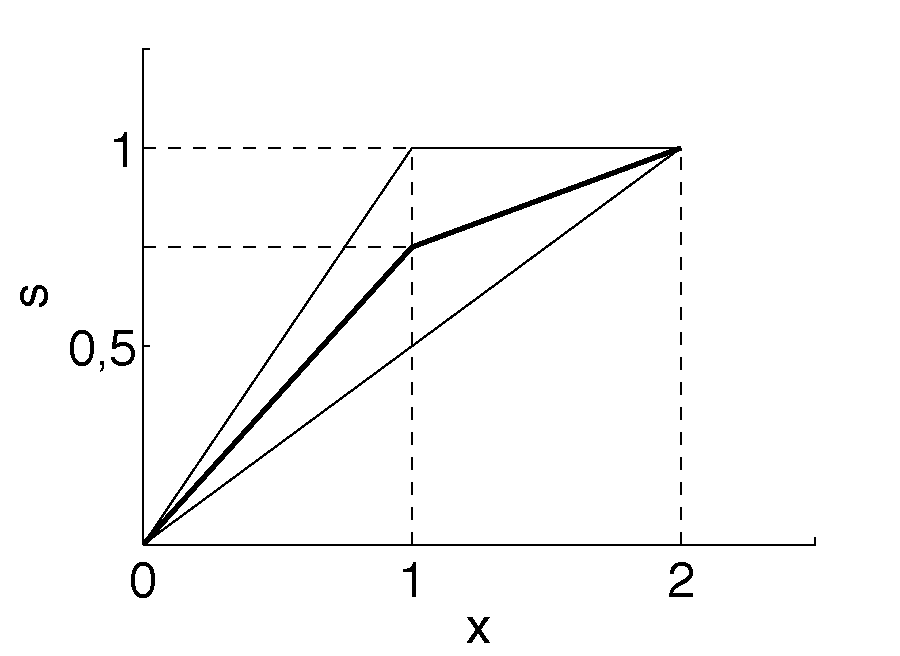
\includegraphics[width=6cm]{Figuras/fig22_1}
			     
%Podr\'{\i}a encontrarse directamente considerando que los cortes para $x$ se hacen sobre una distribuci\'{o}n uniforme, resultan los segmentos  promedio de los bordes.

Como los cortes para cada valor de $X$ se hacen sobre una ddp uniforme, resultan los segmentos promedio de los bordes.
\part $\mathbb E\left\lbrace \left(S-\hat S_\text{MSE}(X)\right)^2 \right\rbrace =\displaystyle\frac{1}{96}$
\part $\hat{S}_\text{LMSE}(X)=\displaystyle\frac{X}{2}+\displaystyle\frac{1}{6}$

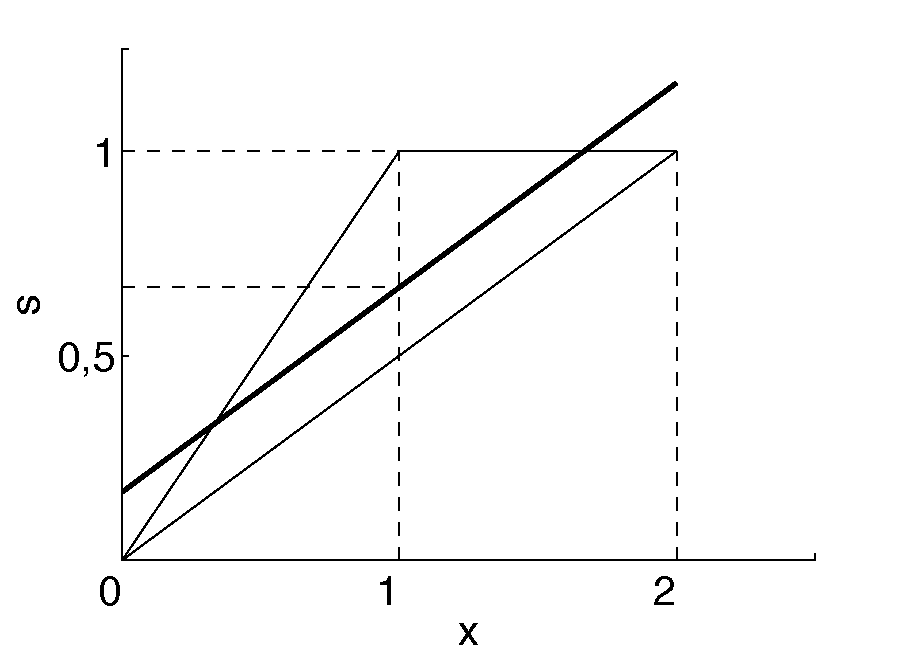
\includegraphics[width=6cm]{Figuras/fig22_2}
\part $\mathbb E\left\lbrace \left(S-\hat S_\text{LMSE}(X)\right)^2 \right\rbrace =\displaystyle\frac{11}{24}$; sensiblemente mayor que $\mathbb E\left\lbrace \left(S-\hat S_\text{MSE}(X)\right)^2 \right\rbrace $ 
\part $\hat{S}_{A,\text{LMSE}}(X)=\displaystyle\frac{3X}{4}$; $\hat{S}_{B,\text{LMSE}}(X)=\displaystyle\frac{1}{2}\left(\displaystyle\frac{X}{2}+1\right)$ que componen $\hat{S}_\text{MSE}(X)$.\\
%\includegraphics[width=6cm]{fig_1.eps}\\
$p_A(s,x)$ y $p_B(s,x)$ son uniformes, y los estimadores \'{o}ptimos lineales y de la forma anterior. 
 \end{parts}
\end{solution}

\else

\question Random variables $S$ and $X$ are characterized by the following joint distribution:
$$p_{S,X}(s,x) = c, \quad 0<s<1, \; \;	  s<x<2s  $$
with $c$ a constant.
\begin{parts}
 		\part Plot the support of the p.d.f., and use it to calculate the value of $c$.
		\part Give the expressions for the marginal p.d.f. of the random variables: $p_S(s)$ and $p_X(x)$.
		\part Find the minimum mean square error estimator of $S$ based on the observation of $X$, $\hat{S}_\text{MSE}(X)$. Plot the estimator on the same plot as the support of $p_{S,X}(s,x)$, and discuss whether it would had been possible to obtain the estimator without analytical derivations.
		\part Calculate the mean square error $\mathbb E\left\lbrace \left(S-\hat S_\text{MSE}(X)\right)^2 \right\rbrace $ incurred by the previous estimator.
		\part Now, find the linear minimum mean square error estimator of $S$ given $X$, $\hat{S}_\text{LMSE}(X)$. Again, plot the estimator together with the support of $p_{S,X}(s,x)$. Discuss your result.
		\part Obtain the mean square error $\mathbb E\left\lbrace \left(S-\hat S_\text{LMSE}(X)\right)^2 \right\rbrace $ of the linear estimator, and compare it with $\mathbb E\left\lbrace \left(S-\hat S_\text{MSE}(X)\right)^2 \right\rbrace $.
		\part It is perceived (e.g., visualizing several samples of $(X,S)$) that there exist different statistical behaviors for $0<X<1$ and $1<X<2$. What would occur if, based on this, different optimal linear estimators where designed for each of the intervals ($\hat{S}_{A,\text{LMSE}}(X)$ y $\hat{S}_{B,\text{LMSE}}(X)$, respectively)? Verify analytically the proposed solution.
\end{parts}

\begin{solution}
\begin{parts}
\part Since the area of the support of $p_{S,X}(s,x)$ is $1/2$, $c=2$.
\part $p_S(s)=2s, \; 0<s<1; \quad \quad p_X(x) =\left\{\begin{array}{ll}\displaystyle  
						  	  x &, 0<x<1\\
	  							2-x &, 1<x<2 
	 					 \end{array} 
						  \right. 
				      $
\part  $\;$ \\

 $ \hat{S}_\text{MSE}(X) =\left\{\begin{array}{ll}\displaystyle  
						  	  \frac{3X}{4}, & 0<X<1\\ \\ \displaystyle  
	  							\frac{1}{2}\left(\frac{X}{2}+1\right), & 1<X<2 
	 					 \end{array} 
						  \right. $
						  
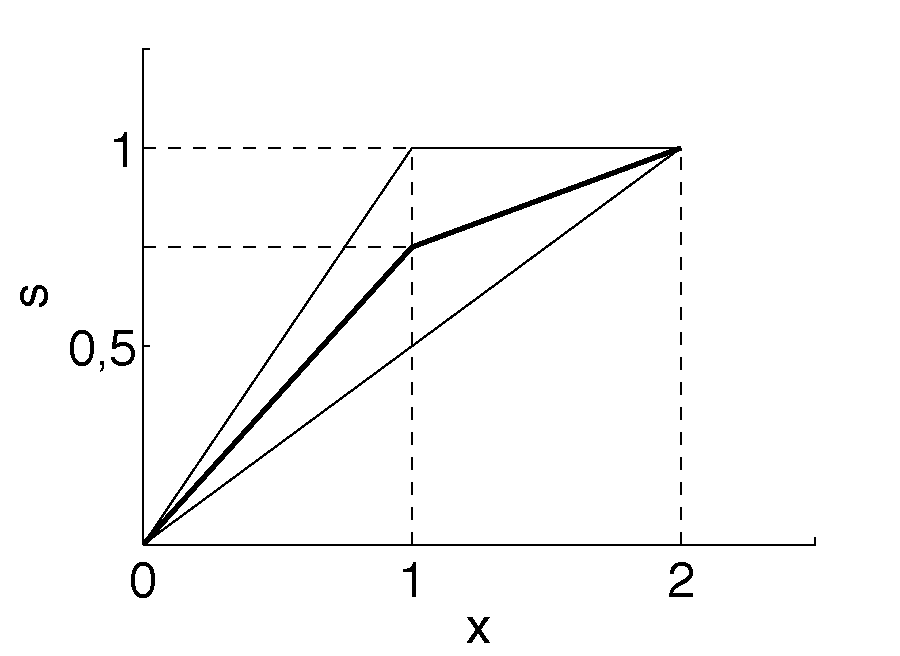
\includegraphics[width=6cm]{Figuras/fig22_1}
			     
%Podr\'{\i}a encontrarse directamente considerando que los cortes para $x$ se hacen sobre una distribuci\'{o}n uniforme, resultan los segmentos  promedio de los bordes.

Since for every value $X$ we have a uniform {\em a posteriori distribution} $p_{S|X}(s|x)$, the MSE estimator is given as the average between the minimum and maximum values of $S$ (for each $X$).
\part $\mathbb E\left\lbrace \left(S-\hat S_\text{MSE}(X)\right)^2 \right\rbrace =\displaystyle\frac{1}{96}$
\part $\hat{S}_\text{LMSE}(X)=\displaystyle\frac{X}{2}+\displaystyle\frac{1}{6}$

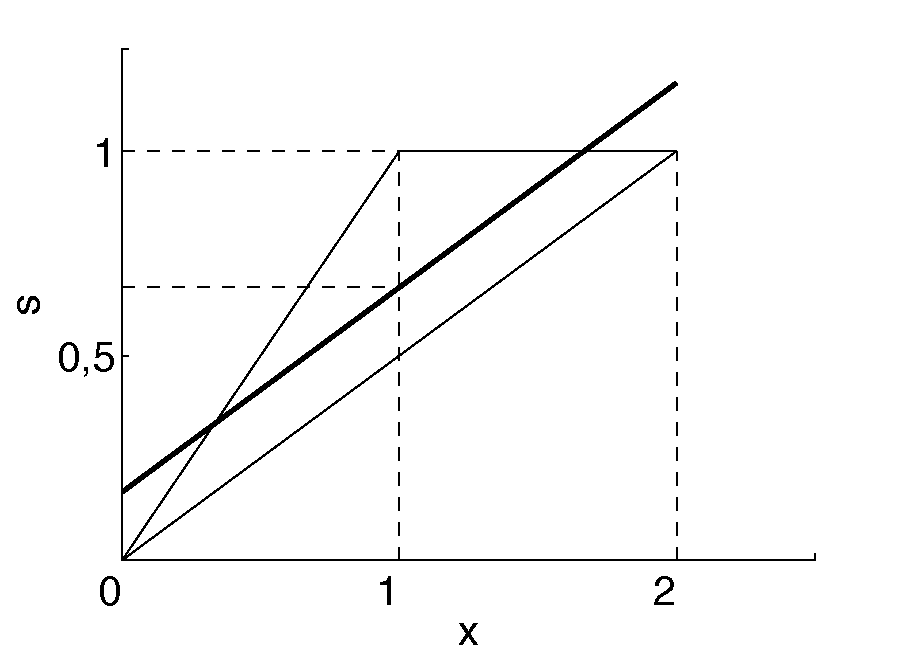
\includegraphics[width=6cm]{Figuras/fig22_2}
\part $\mathbb E\left\lbrace \left(S-\hat S_\text{LMSE}(X)\right)^2 \right\rbrace =\displaystyle\frac{11}{24}$, which is larger than $\mathbb E\left\lbrace \left(S-\hat S_\text{MSE}(X)\right)^2 \right\rbrace $ 
\part $\hat{S}_{A,\text{LMSE}}(X)=\displaystyle\frac{3X}{4}$ and $\hat{S}_{B,\text{LMSE}}(X)=\displaystyle\frac{1}{2}\left(\displaystyle\frac{X}{2}+1\right)$.  When jointly considered, these estimators compose $\hat{S}_\text{MSE}(X)$.\\
%\includegraphics[width=6cm]{fig_1.eps}\\
$p_A(s,x)$ and $p_B(s,x)$ are uniform, and now the linear estimators will also be optimal. 
 \end{parts}
 \end{solution}

\fi

%%%%%%%%%%%%%%%%%%%%%%%%%%%%%%%%%%%%%%%%%%%%%%%%%%%%%%%%%%%%%%%
% 23 Examen TDI/TDS Septiembre 2007 T1
\qformat{\textbf{\ej \thequestion ~~ (1.5; 1.7)} ~~ \linefill}
\ifspanish

\question Se desea estimar un vector aleatorio $\textbf{S}$ a partir de un vector de observaciones $\textbf{X}$ relacionado con él:
$$\textbf{X} = {\bf H} \textbf{S} + \textbf{R}$$
donde $H$ es una matriz conocida, $\textbf{R}$ es un vector de ruido con distribución ${\cal N}(\textbf{0},v_r{\bf I})$, y $\textbf{S}$ es el vector aleatorio a estimar, cuya distribución es ${\cal N}({\bf m_S}, {\bf V_S})$.
Sabiendo que $\textbf{S}$ y $\textbf{R}$ son vectores aleatorios independientes:
\begin{parts}
\part Calcúlese el estimador ML de $\textbf{S}$,  $\mathbf{\hat{S}}_\text{ML}$.
\part Determínese si dicho estimador es sesgado o no. Justifique su respuesta.
\part Según se sabe, el estimador MSE de $\mathbf{S}$ viene dado por la expresión:
$$\mathbf{\hat{S}}_\text{MSE} = \left( {\bf H}^\top{\bf H}  + v_r V_s^{-1}\right) ^{-1} {\bf H}^\top\mathbf{X} $$
Calcúlese el sesgo de $\mathbf{\hat{S}}_\text{MSE} $  e indíquese en qué condiciones dicho sesgo tiende a 0.
\end{parts}

\begin{solution}
\begin{parts}
\part $\mathbf{\hat{S}}_\text{ML}=\left( H^TH  \right) ^{-1} H^T \mathbf{X} $
\part Es insesgado 		
\part $\EE\left\{ \mathbf{\hat{S}}_\text{MSE} - \mathbf{S} \right\}
              = \left({\bf H}^\top{\bf H} + v_r V_s^{-1}\right) ^{-1} {\bf H}^\top{\bf H} \mathbf{m_S}
                - \mathbf{m_S}$.
El sesgo tiende a anularse cuando la potencia de ruido tiende a 0.
\end{parts}
\end{solution}

\else

\question Consider the estimation of a random vector $\textbf{S}$ from a statistically related observation vector $\textbf{X}$:
$$\textbf{X} = {\bf H} \textbf{S} + \textbf{R}$$
where ${\bf H}$ is a known matrix, $\textbf{R}$ a noise vector with distribution ${\cal N}(\textbf{0},v_r{\bf I})$, and $\textbf{S}$ the random vector to be estimated, whose distribution is ${\cal N}({\bf m_S}, {\bf V_S})$.
It is also known that $\textbf{S}$ and $\textbf{R}$ are independent random vectors:
\begin{parts}
\part Find the ML estimator of $\textbf{S}$,  $\mathbf{\hat{S}}_\text{ML}$.
\part Is the ML estimator unbiased? Justify your answer.
\part As it is known, the MSE estimator of $\mathbf{S}$ is given by:
$$\mathbf{\hat{S}}_\text{MSE} = \left( {\bf H}^\top{\bf H}  + v_r {\bf V_S}^{-1}\right) ^{-1} {\bf H}^\top \mathbf{X} $$
Obtain the bias of $\mathbf{\hat{S}}_\text{MSE} $ and indicate under which conditions such bias vanishes.
\end{parts}

\begin{solution}
\begin{parts}
\part $\mathbf{\hat{S}}_\text{ML}=\left( {\bf H}^\top{\bf H} \right) ^{-1} {\bf H}^\top \mathbf{X} $
\part The estimator is unbiased.
\part $\EE\left\{ \mathbf{\hat{S}}_\text{MSE} - \mathbf{S} \right\} = \left( {\bf H}^\top{\bf H}  + v_r {\bf V_S}^{-1}\right) ^{-1} {\bf H}^\top{\bf H} \mathbf{m_S} -\mathbf{m_S}$.
The bias goes to zero as the noise power decreases towards 0.
\end{parts}
\end{solution}

\fi

%%%%%%%%%%%%%%%%%%%%%%%%%%%%%%%%%%%%%%%%%%%%%%%%%%%%%%%%%%%%%%%
% 24 Examen TDI/TDS Septiembre 2007 T3
\qformat{\textbf{\ej \thequestion ~~ (1.4; 1.7)} ~~ \linefill}
\ifspanish

\question Se dispone de $K$ muestras, $\left\{X^{(k)}\right\}^{K}_{k=1}$, tomadas independientemente, de una v.a. X cuya d.d.p. viene dada por 
 	$$p_X(x)=\frac{1}{bx^2} \exp\left(-\frac{1}{bx} \right) u(x) $$
con $b>0$.
\begin{parts}
\part Determínese  $\hat{B}_\text{ML}$ en función de dichas muestras.
\part Verifíquese que la v.a. $Y=1/X$ sigue una d.d.p. $p_Y(y)$  de tipo exponencial unilateral, y establézcase el valor de la media de dicha distribución.
\part Considerando todo lo que antecede, ¿es $\hat{B}_\text{ML}$  un estimador insesgado?
\end{parts}

\begin{solution}
\begin{parts}
\part $\hat{B}_\text{ML}=\displaystyle\frac{1}{K}\displaystyle\sum_{k=1}^K{\displaystyle\frac{1}{X^{(k)}}}$
\part $p_Y(y)=\displaystyle\frac{1}{b} \exp\left(-\displaystyle\frac{y}{b} \right) u(y) $
\part Es insesgado
\end{parts}
\end{solution}

\else

\question We have access to a set of $K$ samples, $\left\{X^{(k)}\right\}^{K}_{k=1}$, independently drawn from a random variable $X$ with p.d.f. 
 	$$p_X(x)=\frac{1}{bx^2} \exp\left(-\frac{1}{bx} \right) u(x) $$
with $b>0$ a constant.
\begin{parts}
\part Find the ML estimator of $b$ as a function of the available samples, $\hat{B}_\text{ML}$.
\part Verify that random variable $Y=1/X$ is characterized by a unilateral exponential p.d.f. $p_Y(y)$, and obtain the value of the mean of such distribution.
\part Considering your answers to the previous sections, is $\hat{B}_\text{ML}$ an unbiased estimator?
\end{parts}

\begin{solution}
\begin{parts}
\part $\hat{B}_\text{ML}=\displaystyle\frac{1}{K}\displaystyle\sum_{k=1}^K{\displaystyle\frac{1}{X^{(k)}}}$
\part $p_Y(y)=\displaystyle\frac{1}{b} \exp\left(-\displaystyle\frac{y}{b} \right) u(y) $
\part The estimator is unbiased.
\end{parts}
\end{solution}

\fi

%%%%%%%%%%%%%%%%%%%%%%%%%%%%%%%%%%%%%%%%%%%%%%%%%%%%%%%%%%%%%%%
% 25 Examen TDI Septiembre 2007 P2
\qformat{\textbf{\ej \thequestion ~~ (1.2)} ~~ \linefill}
\ifspanish

\question Considere la familia de funciones de coste dadas por 
$$
c(S,\hat{S})
    = \frac{1}{N+1} \hat{S}^{N+1} + \frac{1}{N(N+1)} S^{N+1} - \frac1N S \hat{S}^N
$$
siendo $N$ un número entero no negativo e impar. Suponga, asimismo, que
$$
p_{S,X}(s,x) = \frac{1}{\lambda x} \exp\left(-\frac{s}{x} -\frac{x}{\lambda} \right)
\qquad \qquad s \ge 0, \qquad x \ge 0, \qquad \lambda>0 
$$
 
\begin{parts}
\part Determine el estimador de mínimo coste medio de $S$ a la vista de $X$.
\part Determine el mínimo coste medio.
\part Determine el coeficiente $w$ que minimiza el coste medio del estimador de la forma
 $$\hat{S}_L=wX^m$$
siendo $m$ un entero positivo.
\end{parts}
----------------\\
Indicación:  $\int_{0}^{\infty} {x^N} \exp(-x)\; dx=N!$

\begin{solution}
\begin{parts}
\part El riesgo condicional está dado por
\begin{align*}
R_{\hat{s}} &= \EE\{c(S,\hat{s}) | {\bf x} \}  \\
	&= \EE\left\{\frac{1}{N+1} \hat{s}^{N+1} + \frac{1}{N(N+1)} S^{N+1} - \frac1N S \hat{s}^N \mid x \right\}   \\
	&= \frac{1}{N+1} \hat{s}^{N+1} + \frac{1}{N(N+1)} \EE\left\{S^{N+1} \mid x \right\} 
	                               - \frac{1}{N}      \EE\left\{S \mid x\right\} \hat{s}^{N}  
\end{align*}
Dado que este riesgo es una función derivable de $\hat{s}$, su mínimo debe estar en un punto estacionario
\begin{align*}
\frac{\partial R_{\hat{s}}} {\partial \hat{s}} = 0     
& \quad\Leftrightarrow\quad \hat{s}^N  - \EE\left\{S \mid x\right\} \hat{s}^{N-1} = 0            \\
& \quad\Leftrightarrow\quad \hat{s}^{N-1} \left(\hat{s} - \EE\left\{S \mid x\right\} \right) = 0 
\end{align*}
Por tanto, el minimizador del riesgo condicional es
\begin{align*}
\hat{s}^* = \EE\{S \mid x \}.
\end{align*}
Para calcularlo, necesitamos la distribución a posteriori de $S$. Sabiendo que
\begin{align*}
p_X(x) &= \int_{-\infty}^{\infty} p_{S,X}(s, x) ds    
        = \int_0^{\infty} \frac{1}{\lambda x} \exp\left(-\frac{s}{x} -\frac{x}{\lambda} \right) ds    \\
       &= \frac{1}{\lambda x } \exp\left(-\frac{x}{\lambda} \right)  \int_0^{\infty} \exp\left(-\frac{s}{x}\right) ds
        = \frac{1}{\lambda} \exp\left(-\frac{x}{\lambda} \right) 
\end{align*}
resulta
\begin{align*}
p_{S|X}(s|x) = \frac{p_{S,X}(s, x)}{p_{X}(x)} = \frac{1}{x} \exp\left(-\frac{s}{x}\right)
\end{align*} 
y por tanto
\begin{align*}
\hat{s}^* = \EE\{S \mid x \} 
	= \int_{-\infty}^{\infty} s p_{S|X}(s|x) ds
	= \int_0^{\infty} \frac{s}{x} \exp\left(-\frac{s}{x}\right) ds = x
\end{align*}

\part El mínimo riesgo condicional será
\begin{align*}
R_{\hat{s}} &= \frac{1}{N+1} \left(\hat{s}^*\right)^{N+1} + \frac{1}{N(N+1)} \EE\left\{S^{N+1} \mid x \right\} 
	         - \frac1N  \EE\left\{S \mid x\right\} \left(\hat{s}^*\right)^N   \\
	&= \frac{1}{N+1} x^{N+1} + \frac{1}{N(N+1)} \EE\left\{S^{N+1} \mid x \right\} - \frac{1}{N} x^{N+1}   \\
	&= \frac{1}{N(N+1)} \left(\int_0^{\infty} \frac{s^{N+1}}{x} \exp\left(-\frac{s}{x}\right) ds
           	                  - x^{N+1}\right) \\
	&= \frac{(N+1)! - 1}{N(N+1)} x^{N+1} 
\end{align*}
y, por tanto, el riesgo mínimo se puede calcular como
\begin{align*}
\EE\{c(S, \hat{S}\} 
	&= \int_{-\infty}^{\infty} \EE\{c(S,\hat{s}) | {\bf x} \} p_X(x) dx    \\ 
	&= \frac{(N+1)! - 1}{\lambda N(N+1)} \int_0^{\infty}  x^{N+1} \exp\left(-\frac{x}{\lambda} \right) dx    \\ 
	&= \frac{(N+1)! - 1}{N(N+1)}(N+1)! \lambda^{N+1}    \\ 
	&= (N+1)! - 1)(N-1)! \lambda^{N+1}  
\end{align*}
\part Si $\hat{S}=wX^m$, el riesgo será
\begin{align*}
R &= \EE\{c(S,\hat{s}) \}  \\
  &= \frac{1}{N+1} \EE\left\{\hat{S}^{N+1}\right\} + \frac{1}{N(N+1)} \EE\left\{S^{N+1}\right\} - \frac1N \EE\left\{S \hat{S}^N\right\}   \\
  &= \frac{1}{N+1} \EE\left\{X^{m(N+1)}\right\} w^{N+1} + \frac{1}{N(N+1)} \EE\left\{S^{N+1}\right\} 
   - \frac1N \EE\left\{S X^{mN}\right\} w^N  
\end{align*}
Por derivación, esto es mínimo cuando 
\begin{align*}
\EE\left\{X^{m(N+1)}\right\} w^N - \EE\left\{S X^{mN}\right\} w^{N-1} = 0 
\end{align*}
esto es
\begin{align*}
w = \frac{\EE\left\{S X^{mN}\right\}}{\EE\left\{X^{m(N+1)}\right\}}  
\end{align*}
El numerador se puede calcular como
\begin{align*}
\EE\left\{S X^{mN}\right\}
    &= \int_0^\infty \EE\left\{S X^{mN} \mid x \right\} p_X(x) dx    \\
    &= \int_0^\infty x^{mN} \EE\left\{S  \mid x \right\} p_X(x) dx    \\
    &= \frac{1}{\lambda} \int_0^\infty x^{mN+1}  \exp\left(-\frac{x}{\lambda} \right)  dx   
     = \lambda^{mN+1} (mN+1)!
\end{align*}
y el denominador es
\begin{align*}
\EE\left\{X^{m(N+1)}\right\} 
    &= \int_0^\infty x^{m(N+1)} p_X(x) dx    \\
    &= \frac{1}{\lambda} \int_0^\infty x^{m(N+1)} \exp\left(-\frac{x}{\lambda} \right)  dx  
     = \lambda^{m(N+1)} (m(N+1))!
\end{align*}
Por tanto
\begin{align*}
w = \frac{(Nm+1)!}{(Nm+m)!\lambda^{m-1}}
\end{align*}
\end{parts}
\end{solution}

\else

\question Consider the family of cost functions given by
$$
c(S,\hat{S})
    = \frac{1}{N+1} \hat{S}^{N+1} + \frac{1}{N(N+1)} S^{N+1} - \frac{1}{N}S \hat{S}^N
$$
where $N$ is a non-negative and odd integer, and assume that
$$
p_{S,X}(s,x) = \frac{1}{\lambda x} \exp\left(-\frac{s}{x} -\frac{x}{\lambda} \right)
\qquad \qquad s \ge 0, \qquad x \ge 0, \qquad \lambda>0 
$$

\begin{parts}
\part Find the minimum mean cost estimator of $S$ given $X$.
\part Obtain the minimum mean cost.
\part Determine the coefficient $w$ that minimizes the mean cost of an estimator with analytical shape
 $$\hat{S}_L=wX^m$$
$m$ being a positive integer.
\end{parts}
----------------\\
Hint:  $\int_{0}^{\infty} x^N \exp(-x)\; dx=N!$

\begin{solution}
\begin{parts}
\part The conditional risk is given by
\begin{align*}
R_{\hat{s}} &= \EE\{c(S,\hat{s}) | {\bf x} \}  \\
	&= \EE\left\{\frac{1}{N+1} \hat{s}^{N+1} + \frac{1}{N(N+1)} S^{N+1} - \frac1N S \hat{s}^N \mid x \right\}   \\
	&= \frac{1}{N+1} \hat{s}^{N+1} + \frac{1}{N(N+1)} \EE\left\{S^{N+1} \mid x \right\} 
	                               - \frac{1}{N}      \EE\left\{S \mid x\right\} \hat{s}^{N}  
\end{align*}
Since this risk is a differentiable function of $\hat{s}$, the minimum must be at a stationary point
\begin{align*}
\frac{\partial R_{\hat{s}}} {\partial \hat{s}} = 0     
& \quad\Leftrightarrow\quad \hat{s}^N  - \EE\left\{S \mid x\right\} \hat{s}^{N-1} = 0            \\
& \quad\Leftrightarrow\quad \hat{s}^{N-1} \left(\hat{s} - \EE\left\{S \mid x\right\} \right) = 0 
\end{align*}
Thus the minimizer of the conditional risk is
\begin{align*}
\hat{s}^* = \EE\{S \mid x \}.
\end{align*}
To compute the conditional mean, we need the posterior distribution of $S$. Noting that
\begin{align*}
p_X(x) &= \int_{-\infty}^{\infty} p_{S,X}(s, x) ds    
        = \int_0^{\infty} \frac{1}{\lambda x} \exp\left(-\frac{s}{x} -\frac{x}{\lambda} \right) ds    \\
       &= \frac{1}{\lambda x } \exp\left(-\frac{x}{\lambda} \right)  \int_0^{\infty} \exp\left(-\frac{s}{x}\right) ds
        = \frac{1}{\lambda} \exp\left(-\frac{x}{\lambda} \right) 
\end{align*}
we have
\begin{align*}
p_{S|X}(s|x) = \frac{p_{S,X}(s, x)}{p_{X}(x)} = \frac{1}{x} \exp\left(-\frac{s}{x}\right)
\end{align*} 
so that
\begin{align*}
\hat{s}^* = \EE\{S \mid x \} 
	= \int_{-\infty}^{\infty} s p_{S|X}(s|x) ds
	= \int_0^{\infty} \frac{s}{x} \exp\left(-\frac{s}{x}\right) ds = x
\end{align*}

\part Since the minimum conditional risk is
\begin{align*}
R_{\hat{s}} &= \frac{1}{N+1} \left(\hat{s}^*\right)^{N+1} + \frac{1}{N(N+1)} \EE\left\{S^{N+1} \mid x \right\} 
	         - \frac1N  \EE\left\{S \mid x\right\} \left(\hat{s}^*\right)^N   \\
	&= \frac{1}{N+1} x^{N+1} + \frac{1}{N(N+1)} \EE\left\{S^{N+1} \mid x \right\} - \frac{1}{N} x^{N+1}   \\
	&= \frac{1}{N(N+1)} \left(\int_0^{\infty} \frac{s^{N+1}}{x} \exp\left(-\frac{s}{x}\right) ds
           	                  - x^{N+1}\right) \\
	&= \frac{(N+1)! - 1}{N(N+1)} x^{N+1} 
\end{align*}
the minimum risk can be computed as
\begin{align*}
\EE\{c(S, \hat{S}\} 
	&= \int_{-\infty}^{\infty} \EE\{c(S,\hat{s}) | {\bf x} \} p_X(x) dx    \\ 
	&= \frac{(N+1)! - 1}{\lambda N(N+1)} \int_0^{\infty}  x^{N+1} \exp\left(-\frac{x}{\lambda} \right) dx    \\ 
	&= \frac{(N+1)! - 1}{N(N+1)}(N+1)! \lambda^{N+1}    \\ 
	&= (N+1)! - 1)(N-1)! \lambda^{N+1}  
\end{align*}
\part If $\hat{S}=wX^m$, the risk is given by
\begin{align*}
R &= \EE\{c(S,\hat{s}) \}  \\
  &= \frac{1}{N+1} \EE\left\{\hat{S}^{N+1}\right\} + \frac{1}{N(N+1)} \EE\left\{S^{N+1}\right\} - \frac1N \EE\left\{S \hat{S}^N\right\}   \\
  &= \frac{1}{N+1} \EE\left\{X^{m(N+1)}\right\} w^{N+1} + \frac{1}{N(N+1)} \EE\left\{S^{N+1}\right\} 
   - \frac1N \EE\left\{S X^{mN}\right\} w^N  
\end{align*}
By differentiation, this is minimum when
\begin{align*}
\EE\left\{X^{m(N+1)}\right\} w^N - \EE\left\{S X^{mN}\right\} w^{N-1} = 0 
\end{align*}
that is
\begin{align*}
w = \frac{\EE\left\{S X^{mN}\right\}}{\EE\left\{X^{m(N+1)}\right\}}  
\end{align*}
The numerator can be computed as
\begin{align*}
\EE\left\{S X^{mN}\right\}
    &= \int_0^\infty \EE\left\{S X^{mN} \mid x \right\} p_X(x) dx    \\
    &= \int_0^\infty x^{mN} \EE\left\{S  \mid x \right\} p_X(x) dx    \\
    &= \frac{1}{\lambda} \int_0^\infty x^{mN+1}  \exp\left(-\frac{x}{\lambda} \right)  dx   
     = \lambda^{mN+1} (mN+1)!
\end{align*}
and the denominator is
\begin{align*}
\EE\left\{X^{m(N+1)}\right\} 
    &= \int_0^\infty x^{m(N+1)} p_X(x) dx    \\
    &= \frac{1}{\lambda} \int_0^\infty x^{m(N+1)} \exp\left(-\frac{x}{\lambda} \right)  dx  
     = \lambda^{m(N+1)} (m(N+1))!
\end{align*}
Therefore
\begin{align*}
w = \frac{(Nm+1)!}{(Nm+m)!\lambda^{m-1}}
\end{align*}
\end{parts}
\end{solution}

\fi

%%%%%%%%%%%%%%%%%%%%%%%%%%%%%%%%%%%%%%%%%%%%%%%%%%%%%%%%%%%%%%%
% 26 Examen TDI/TDS Junio 2007 T1
\qformat{\textbf{\ej \thequestion ~~ (1.4; 1.7)} ~~ \linefill}
\ifspanish

\question La densidad de probabilidad tipo Erlang de orden $N$ viene dada por la expresión
 $$p_X(x)=\frac{a^N x^{N-1} \exp (-ax)}{(N-1)!} \quad  x >0, \quad   a>0 $$
Supóngase que $N$ es conocida. Considerando que la media viene dada por $m = N/a$, determine: 
\begin{parts}
\part El estimador ML de la media, $\hat{M}_\text{ML}$, a partir de $K$ observaciones independientes de la variable.
\part El sesgo condicional de $\hat{M}_\text{ML}$.
\part ¿Es $\hat{M}_\text{ML}$ un estimador consistente en MSE?
\end{parts}

\begin{solution}
\begin{parts}
\part $\hat{M}_\text{ML}=\dfrac{1}{K}\sum_{k=1}^K X_k$
\part Es insesgado 
\part $\text{var}\left\{ \hat{M}_\text{ML}\right\} =\dfrac{v_x}{K}$, luego es consistente en MSE
\end{parts}
\end{solution}

\else

\question An order-$N$ Erlang probability density is characterized by the following expression:
  $$p_X(x)=\frac{a^N x^{N-1} \exp (-ax)}{(N-1)!} \quad  x >0, \quad   a>0 $$
Assume that $N$ is known.  Considering that the mean of the distribution is given by $m = N/a$, obtain: 
\begin{parts}
\part The ML estimator of the mean using $K$ independent observations of the variable, $\hat{M}_\text{ML}$.
\part The conditional bias of $\hat{M}_\text{ML}$.
\part Is $\hat{M}_\text{ML}$ MSE-consistent?
\end{parts}

\begin{solution}
\begin{parts}
\part $\hat{M}_\text{ML}=\dfrac{1}{K}\sum_{k=1}^K X_k$
\part The estimator is unbiased.
\part $\text{var}\left\{ \hat{M}_\text{ML}\right\} =\dfrac{v_x}{K}$; therefore, the estimator is MSE-consistent.
\end{parts}
\end{solution}

\fi

%%%%%%%%%%%%%%%%%%%%%%%%%%%%%%%%%%%%%%%%%%%%%%%%%%%%%%%%%%%%%%%
% 27 Examen TDI Febrero 2007 T1
\qformat{\textbf{\ej \thequestion ~~ (1.6)} ~~ \linefill}
\ifspanish

\question La variable $X=[X_1, X_2, X_3]^T$ se distribuye según una ddp de media $\mathbf{m}=\mathbf{0}$ y matriz de covarianza 
 $$V_{XX}=\left[ \begin{array}{ccc}\displaystyle  
						  	  3& 2 & 1\\
						  	  2& 3 & 2\\
						  	  1 & 2 & 3\end{array}    \right] $$
\begin{parts}
\part Calcúlense los coeficientes ($w_0$, $w_1$ y $w_2$) del estimador lineal de error cuadrático medio mínimo de $X_3$ a la vista de $X_1$ y $X_2$,
 $$\hat{X}_{3,\text{LMSE}}=w_0+w_1X_1+w_2X_2$$
\part Calcúlese el error cuadrático medio $\mathbb E\left\lbrace \left( X_3-\hat{X}_{3,\text{LMSE}}\right)^2 \right\rbrace$.
\end{parts}

\begin{solution}
\begin{parts}
\part $\hat{X}_{3,\text{LMSE}}=-\displaystyle\frac{1}{5}X_1+\displaystyle\frac{4}{5}X_2$
\part $\mathbb E\left\lbrace \left( X_3-\hat{X}_{3,\text{LMSE}}\right)^2 \right\rbrace=\displaystyle\frac{8}{5}$
\end{parts}
\end{solution}

\else

\question Random vector $X=[X_1, X_2, X_3]^T$ follows a p.d.f. with mean $\mathbf{m}=\mathbf{0}$ and covariance matrix
 $$V_{XX}=\left[ \begin{array}{ccc}\displaystyle  
						  	  3& 2 & 1\\
						  	  2& 3 & 2\\
						  	  1 & 2 & 3\end{array}    \right] $$
\begin{parts}
\part Obtain the coefficients ($w_0$, $w_1$ and $w_2$) of the linear minimum mean square error estimator of $X_3$ given $X_1$ and $X_2$,
 $$\hat{X}_{3,\text{LMSE}}=w_0+w_1X_1+w_2X_2$$
\part Calculate the mean square error of the estimator $\mathbb E\left\lbrace \left( X_3-\hat{X}_{3,\text{LMSE}}\right)^2 \right\rbrace$.
\end{parts}

\begin{solution}
\begin{parts}
\part $\hat{X}_{3,\text{LMSE}}=-\displaystyle\frac{1}{5}X_1+\displaystyle\frac{4}{5}X_2$
\part $\mathbb E\left\lbrace \left( X_3-\hat{X}_{3,\text{LMSE}}\right)^2 \right\rbrace=\displaystyle\frac{8}{5}$
\end{parts}
\end{solution}

\fi

%%%%%%%%%%%%%%%%%%%%%%%%%%%%%%%%%%%%%%%%%%%%%%%%%%%%%%%%%%%%%%%
%  Examen TDI Febrero 2007 P1
\qformat{\textbf{\ej \thequestion ~~ (1.4)} ~~ \linefill}
\ifspanish

\question La v.a. $X$ con ddp
$$ p_X(x) = \left\{\begin{array}{ll}
				   1, & 0<x<1 \\
	    			   0, & {\mbox{en otro caso}} 
	 		       \end{array} 
			\right.$$
se transforma como indica en la figura, dando lugar a la v.a. observable $Y$.

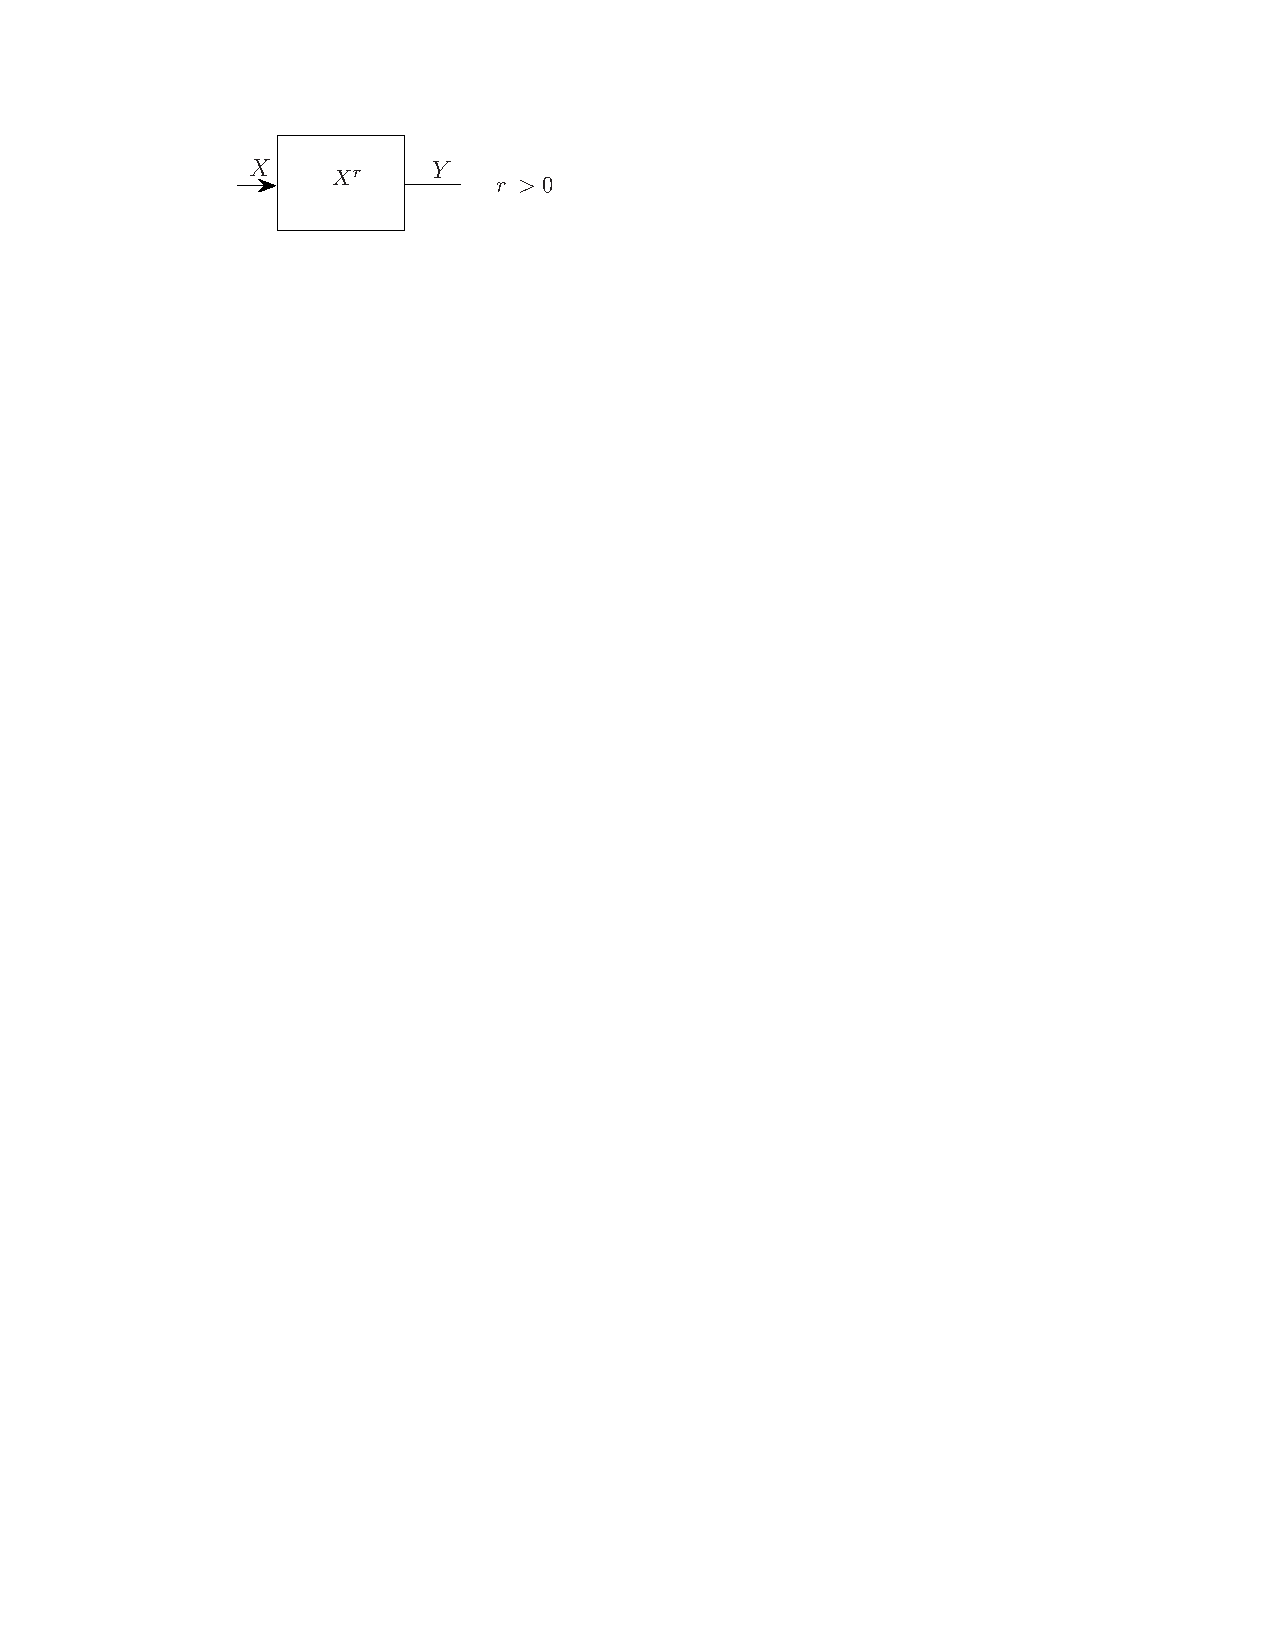
\includegraphics[width=8cm, trim=0 24cm 12cm 2cm]{Figuras/fig28_1}

\begin{parts}
	\part Obt\'{e}ngase el estimador de m\'{a}xima verosimilitud de $r$, $\hat{R}_\text{ML}$, a partir de $K$ observaciones de $Y$ tomadas de forma independiente.
	\part Considere la situaci\'{o}n \\

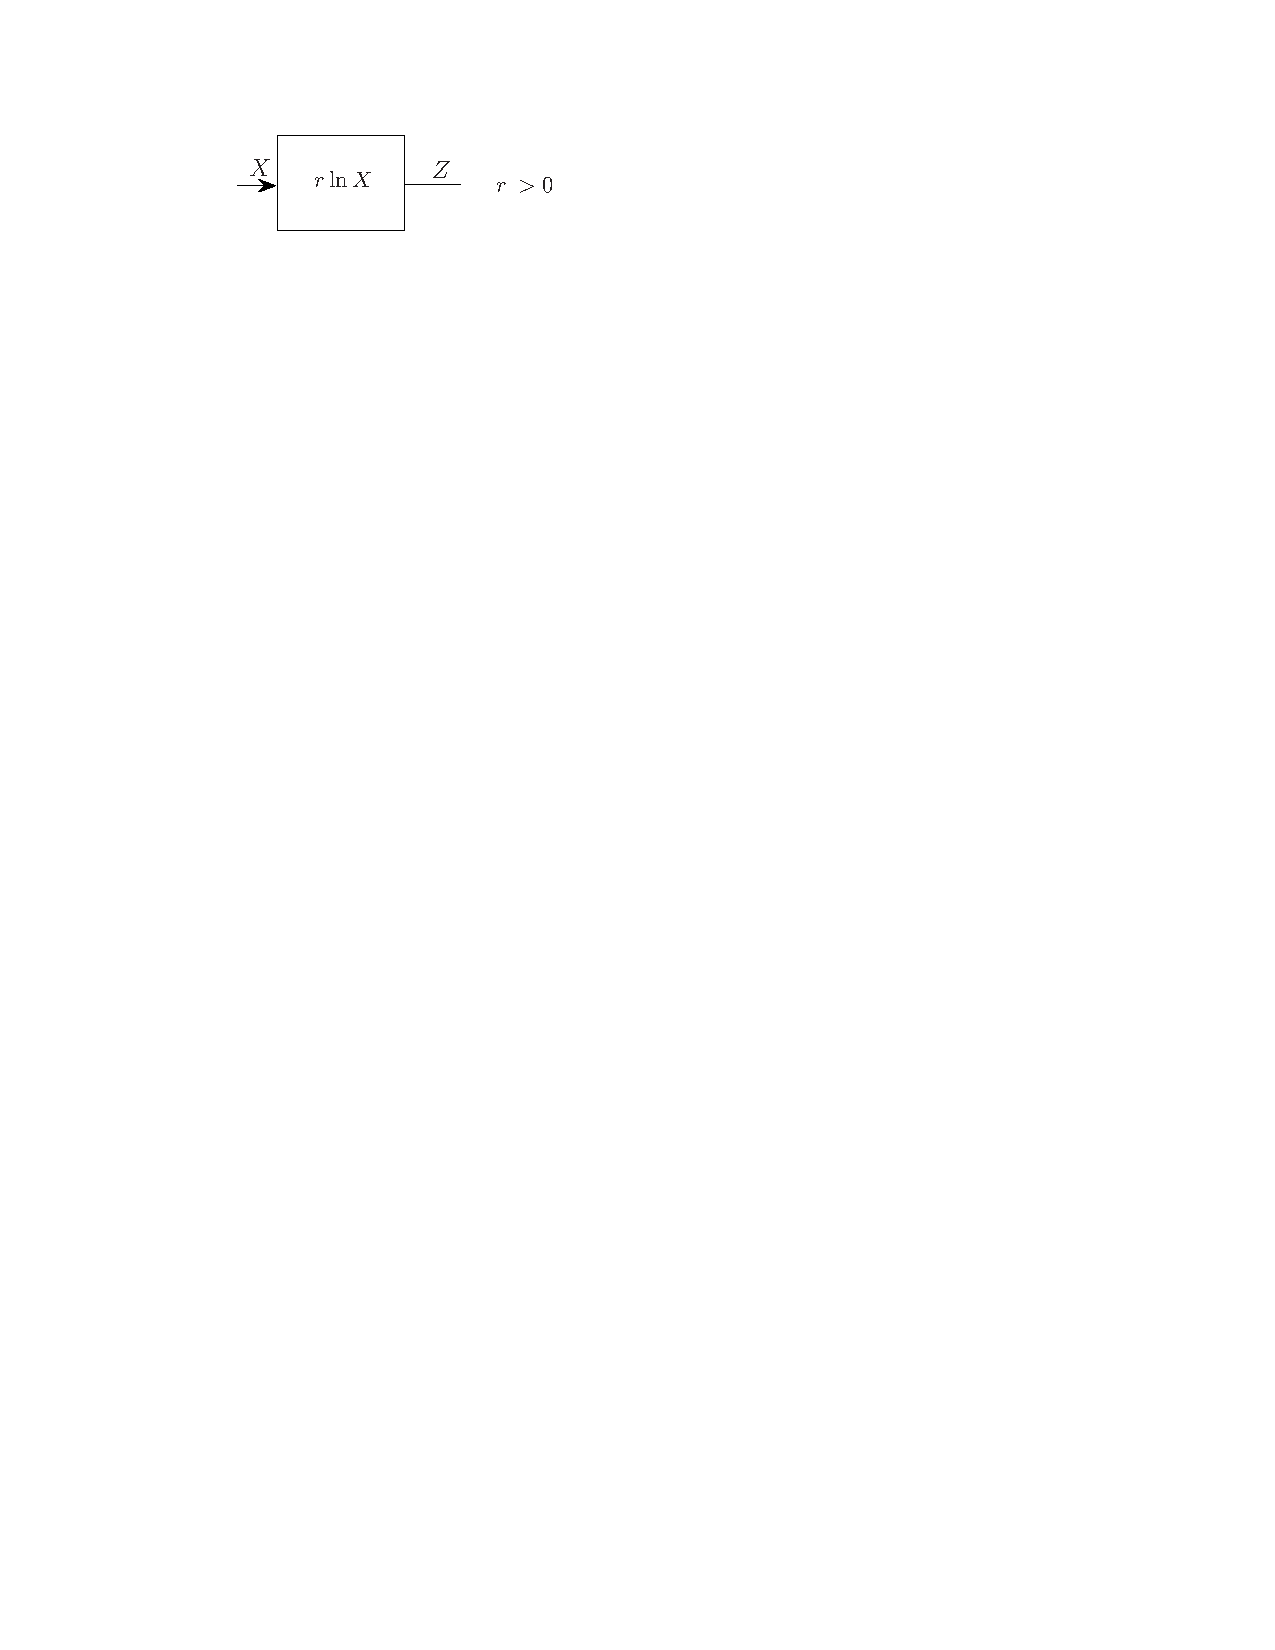
\includegraphics[width=8cm, trim=0 24cm 12cm 2cm]{Figuras/fig28_2}

y obtenga $\hat{R}_\text{ML}$ de $K$ observaciones de $Z$ tomadas independientemente. Comente el resultado.
\end{parts}				


\begin{solution} 
  \begin{parts}
  \part $\hat{R}_\text{ML} = -\frac{1}{K}\sum^{K-1}_{k=0}\ln Y_k$.  Se est\'{a} identificando el par\'{a}metro desconocido de la transformaci\'{o}n.
  \part $\hat{R}_\text{ML} = -\frac{1}{K} \sum^{K-1}_{k=0} Z_k$. Coincide con el anterior: $Z=\ln Y$, ya que implica una transformaci\'{o}n invertible de $Y$. 
  \end{parts}
\end{solution}

\else

\question A random variable $X$ with p.d.f.
$$ p_X(x) = \left\{\begin{array}{ll}
				  1, & 0<x<1 \\
	  			  0, & {\mbox{otherwise}} 
	 			 \end{array} 
		  \right.  $$
is transformed as indicated in the figure, producing a random observation $Y$.

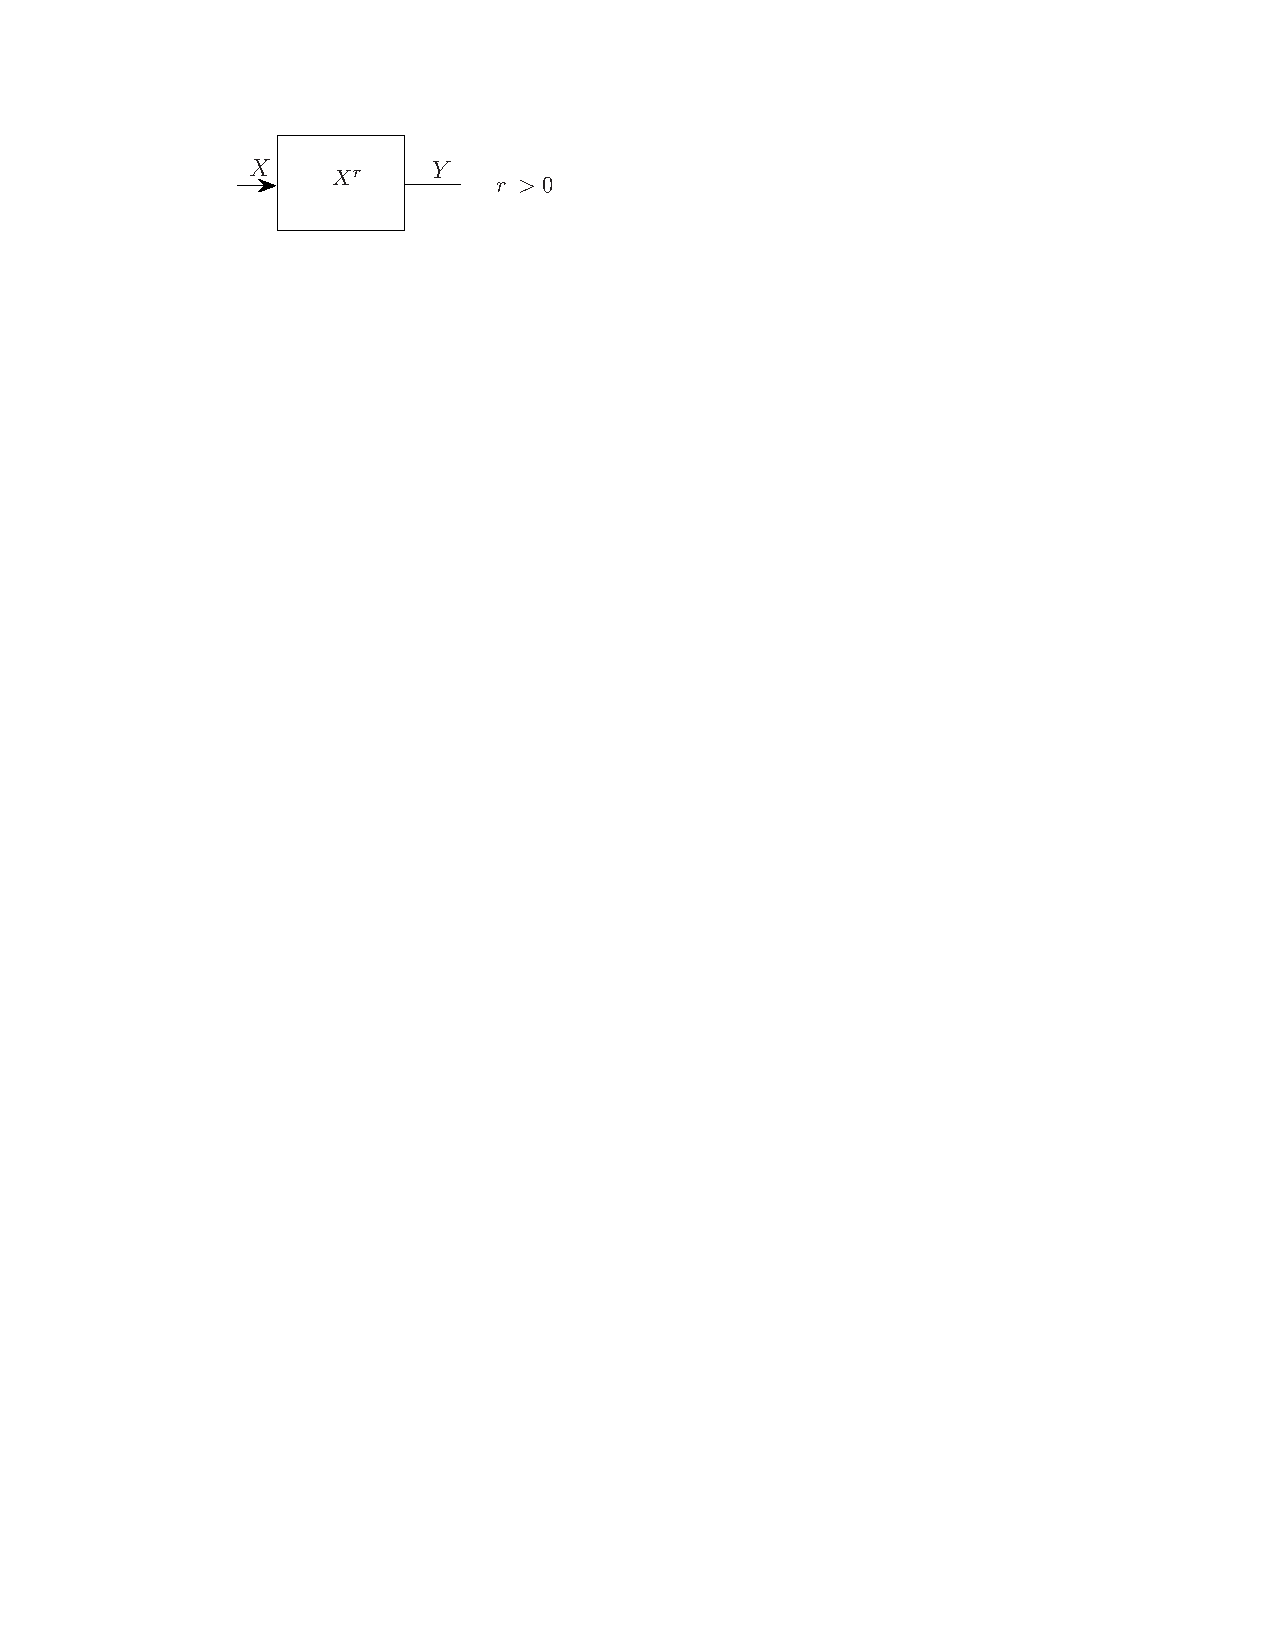
\includegraphics[width=8cm, trim=0 24cm 12cm 2cm]{Figuras/fig28_1}

\begin{parts}
\part Obtain the maximum likelihood estimator of $r$, $\hat{R}_\text{ML}$, based on $K$  independently drawn observations of $Y$.
\part Now, consider the following situation \\

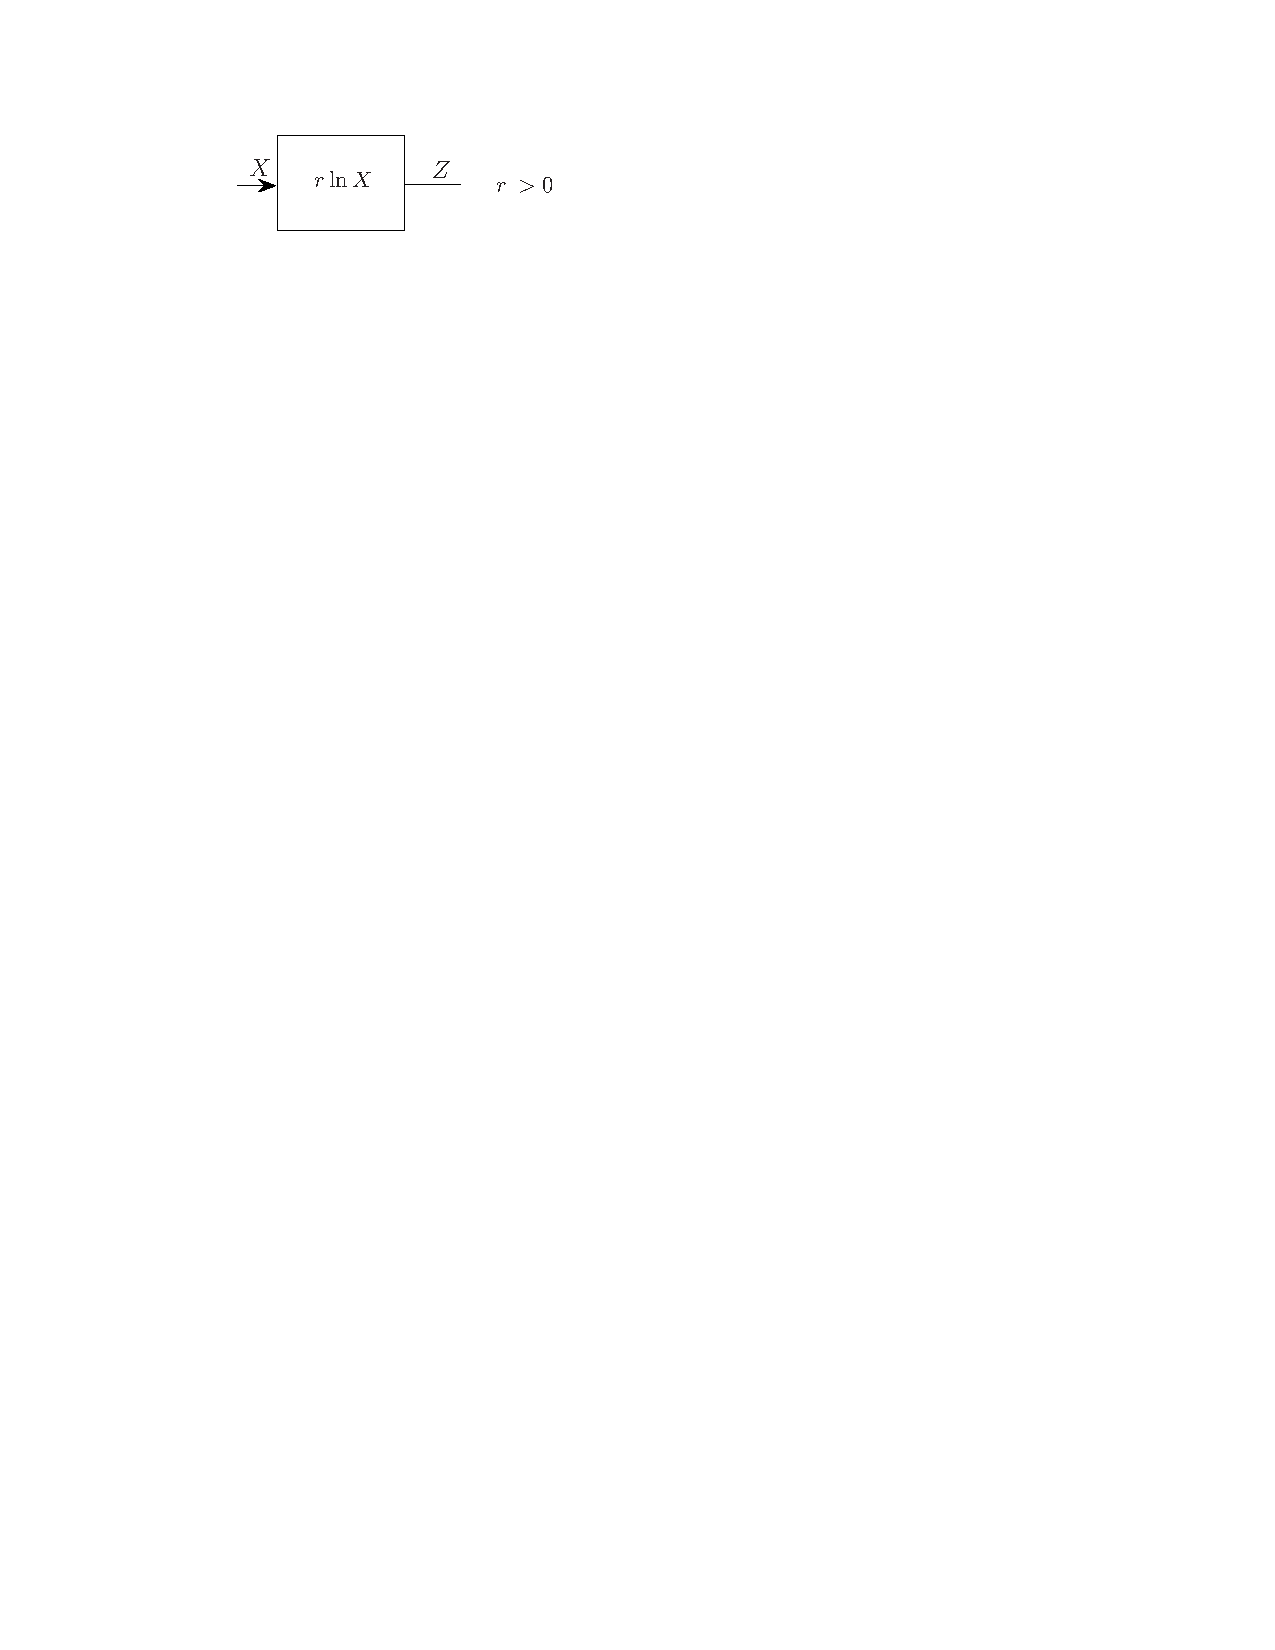
\includegraphics[width=8cm, trim=0 24cm 12cm 2cm]{Figuras/fig28_2}

and obtain $\hat{R}_\text{ML}$ using $K$ independent observations of random variable $Z$.  Discuss your result.
\end{parts}				

\begin{solution} 
\begin{parts}
\part $\hat{R}_\text{ML}=-\frac{1}{K} \sum^{K-1}_{k=0}\ln Y_k$. The unknown parameter of the transformation is being identified.
\part $\hat{R}_\text{ML}=-\frac{1}{K} \sum^{K-1}_{k=0} Z_k$. It is coherent with the previous estimator since $Z=\ln Y$, which is a deterministic (and invertible) transformation of $Y$. 
\end{parts}
\end{solution}

\fi

%%%%%%%%%%%%%%%%%%%%%%%%%%%%%%%%%%%%%%%%%%%%%%%%%%%%%%%%%%%%%%%
%  Examen TDI Enero 2007 P1 (convocatoria extraordinaria)
\qformat{\textbf{\ej \thequestion ~~ (1.4)} ~~ \linefill}
\ifspanish

\question Se mide el par\'{a}metro determinista desconocido $s$, $s>0$, mediante dos sistemas, que proporcionan las observaciones
$$X_i=A_{i}s+N_i,	\quad	i=1,2$$

siendo $\left\{A_i\right\},\left\{N_i\right\}$, vv.aa. gaussianas e independientes entre s\'{\i}, con medias $\mathbb E\left\{A_i\right\}=1$, $\mathbb E\left\{N_i\right\}=0$, y varianzas $\left\{v_{Ai}\right\}$, $\left\{v_{Ni}\right\}$, respectivamente ($i=1,2$).
\begin{parts}
	\part Establ\'{e}zcase la expresi\'{o}n que proporciona el estimador ML de $s$, $\hat{S}_\text{ML}$.
	\part Calc\'{u}lese $\hat{S}_\text{ML}$ para el caso particular $v_{Ai}=0, i=1,2$.
	\part Calc\'{u}lese $\hat{S}_\text{ML}$ para el caso particular $v_{Ni}=0, i=1,2$.
\end{parts}

\begin{solution}   
  \begin{parts}
  \part $\hat{S}_\text{ML}=\mbox{arg}\ \min_{s} \left\{\ln\left[(s^{2}v_{A1}+v_{N1})(s^{2}v_{A2}+v_{N2})\right]+\displaystyle\frac{(s-X_1)^{2}}{s^{2}v_{A1}+v_{N1}}	+\displaystyle\frac{(s-X_2)^{2}}{s^{2}v_{A2}+v_{N2}}\right\}$
  \part $\hat{S}_\text{ML}=\displaystyle\frac{v_{N2}X_{1}+v_{N1}X_{2}}{v_{N1}+v_{N2}}$
  \part $\hat{S}_\text{ML}=\displaystyle\frac{1}{4}\sqrt{\left(\displaystyle\frac{X_{1}}{v_{A1}}+\displaystyle\frac{X_{2}}{v_{A2}}\right)^{2}+
  8\left(\displaystyle\frac{X_{1}^2}{v_{A1}}+\displaystyle\frac{X_{2}^2}{v_{A2}}\right)}-\left( \displaystyle\frac{X_{1}}{v_{A1}}+\displaystyle\frac{X_{2}}{v_{A2}}\right) $
\end{parts}
\end{solution}

\else

\question An unknown deterministic parameter $s$, $s>0$ is measured using two different systems, which provide observations
$$X_i=A_{i}s+N_i,	\quad	i=1,2$$

where $\left\{A_i\right\},\left\{N_i\right\}$, are independent Gaussian random vectors, with means $\mathbb E\left\{A_i\right\}=1$, $\mathbb E\left\{N_i\right\}=0$, and variances $\left\{v_{Ai}\right\}$, $\left\{v_{Ni}\right\}$, respectively ($i=1,2$).
\begin{parts}
	\part Stablish the expression that defines the ML estimator of $s$, $\hat{S}_\text{ML}$.
	\part Obtain $\hat{S}_\text{ML}$ for the particular case $v_{Ai}=0, i=1,2$.
	\part Obtain $\hat{S}_\text{ML}$ for the particular case $v_{Ni}=0, i=1,2$.
\end{parts}

\begin{solution}
  \begin{parts}
  \part $\hat{S}_\text{ML}=\mbox{arg}\ \min_{s} \left\{\ln\left[(s^{2}v_{A1}+v_{N1})(s^{2}v_{A2}+v_{N2})\right]+\displaystyle\frac{(s-X_1)^{2}}{s^{2}v_{A1}+v_{N1}}	+\displaystyle\frac{(s-X_2)^{2}}{s^{2}v_{A2}+v_{N2}}\right\}$
  \part $\hat{S}_\text{ML}=\displaystyle\frac{v_{N2}X_{1}+v_{N1}X_{2}}{v_{N1}+v_{N2}}$
  \part $\hat{S}_\text{ML}=\displaystyle\frac{1}{4}\sqrt{\left(\displaystyle\frac{X_{1}}{v_{A1}}+\displaystyle\frac{X_{2}}{v_{A2}}\right)^{2}+
  8\left(\displaystyle\frac{X_{1}^2}{v_{A1}}+\displaystyle\frac{X_{2}^2}{v_{A2}}\right)}-\left( \displaystyle\frac{X_{1}}{v_{A1}}+\displaystyle\frac{X_{2}}{v_{A2}}\right) $
\end{parts}
\end{solution}

\fi

%%%%%%%%%%%%%%%%%%%%%%%%%%%%%%%%%%%%%%%%%%%%%%%%%%%%%%%%%%%%%%%
% Examen TDI Mayo 2010 P2
\qformat{\textbf{\ej \thequestion ~~ (1.3; 1.6)} ~~ \linefill}
\ifspanish

\question 
Sean $X$ y $S$ dos variables aleatorias con d.d.p. conjunta 
\begin{equation}
p_{X,S}(x,s) 
	= \left \{\begin{array}{ll} 
	          \alpha & ;\;\;\; 0<x<1,\ 0<s<2(1-x) \\
	          0      & ;\;\;\; \mbox{otherwise}
	          \end{array} \right.  \nonumber
\end{equation}
siendo $\alpha$ una constante.
\begin{parts}
\part Utilizando la representación del soporte de la d.d.p., determine el valor de $\alpha$.
\part Encuentre la función de densidad de probabilidad de $S$ a la vista de $X$, $p_{S|X}(s|x)$.
\part Calcule el estimador de mínimo error cuadrático medio de $S$ a la vista de $X$, $\SMSE$
\part Calcule el estimador lineal de mínimo error cuadrático medio de $S$ a la vista de $X$, $\SLMSE$.
\end{parts}

\begin{solution}
\begin{parts}
\part $\alpha=1$
\part $p_{S|X}(s|x)=\frac{1}{2\left(1-x \right) }$
\part $\SMSE=1-X$
\part $\SLMSE=1-X$
\end{parts}
\end{solution}


\else

\question 
Let $X$ and $S$ be two random variables with joint pdf 
\begin{equation}
p_{X,S}(x,s) 
	= \left \{\begin{array}{ll} 
	          \alpha & ;\;\;\; 0<x<1,\ 0<s<2(1-x) \\
	          0      & ;\;\;\; \mbox{otherwise}
	          \end{array} \right.  \nonumber
\end{equation}
with $\alpha$ a constant.
\begin{parts}
\part Plot the support of the pdf, and use it to determine the value of $\alpha$.
\part Obtain the posterior pdf of $S$ given $X$, $p_{S|X}(s|x)$.
\part Find the minimum mean square error estimator of $S$ given $X$, $\SMSE$
\part Find the linear minimum mean square error estimator of $S$ given $X$, $\SLMSE$.
\end{parts}

\begin{solution}
\begin{parts}
\part $\alpha=1$
\part $p_{S|X}(s|x)=\frac{1}{2\left(1-x \right) }$
\part $\SMSE=1-X$
\part $\SLMSE=1-X$
\end{parts}
\end{solution}

\fi
 
%%%%%%%%%%%%%%%%%%%%%%%%%%%%%%%%%%%%%%%%%%%%%%%%%%%%%%%%%%%%%%%
% Examen TDI Mayo 2010 P4
\qformat{\textbf{\ej \thequestion ~~ (1.3; 1.4; 1.7)} ~~ \linefill}
\ifspanish

\question 
Para la estimación de una variable aleatoria $S$ se dispone de una observación de la v.a. $X$ caracterizada por:
$$X=S+N$$
siendo la función de densidad de probabilidad de $S$
$$p_S(s)=s\exp(-s) \quad s \ge 0$$
y $N$ un ruido aditivo, independiente de $S$, con distribución
$$p_N(n)=\exp(-n) \quad n \ge 0$$.
\begin{parts}
\part Obtenga el estimador de máxima verosimilitud de $S$, $\widehat{S}_\text{ML}$.
\part Determine la función de densidad de probabilidad conjunta de $X$ y $S$, $p_{X,S}(x,s)$, y la función de densidad de probabilidad de $S$ a la vista de $X$, $p_{S|X}(s|x)$.
\part Obtenga el estimador máximo a posteriori de $S$ a la vista de $X$, $\widehat{S}_\text{MAP}$.
\part Obtenga el estimador de mínimo error cuadrático medio de $S$ a la vista de $X$, $\widehat{S}_\text{MSE}$.
\part Calcule el sesgo de los estimadores obtenidos anteriormente, $\widehat{S}_\text{ML}$, $\widehat{S}_\text{MAP}$ y $\widehat{S}_\text{MSE}$.
\part Indique qué estimador tiene una menor varianza. Razone la respuesta sin calcular las varianzas de los estimadores.
\end{parts}
\vspace{.2cm}
Nota: Para la resolución del ejercicio puede emplear la siguiente igualdad:
$$\int_0^{\infty} \! x^N\exp(-x) \, dx=N!$$

\begin{solution}
  \begin{parts}
 \part  $\widehat{S}_\text{ML}=X$
 \part $\displaystyle p_{X,S}(x,s) = s \exp (-x) \quad x \ge s, \; s \ge 0$\\
 $\displaystyle p_{S|X}(s|x)= \frac{2s}{x^2} \quad 0 \le s \le x,\; x \ge 0$
 \part  $\widehat{S}_\text{MAP}=X$
 \part  $\displaystyle \widehat{S}_\text{MSE}=\frac{2}{3}X$
 \part $\mathbb E \left\lbrace S- \widehat S_{\text{ML}}  \right\rbrace= \mathbb E \left\lbrace S- \widehat S_{\text{MAP}} \right\rbrace = -1$ \\
 $\mathbb{E} \left\lbrace S- \widehat S_{\text{MSE}}  \right\rbrace= 0 $\\
  $ \displaystyle {\rm Var} \left\lbrace \widehat S_{\text{MSE}}  \right\rbrace < {\rm Var} \left\lbrace  \widehat S_{\text{MAP}}  \right\rbrace= {\rm Var} \left\lbrace  \widehat S_{\text{ML}}  \right\rbrace$

 \end{parts}
 \end{solution}

\else

\question 
Consider an estimation problem where the goal is to estimate a random variable $S$ using an observation of another random variable $X$ characterized by:
$$X=S+N$$
where the prior pdf of $S$ is
$$p_S(s)=s\exp(-s) \quad s \ge 0$$
and where $N$ is an additive noise, independent of $S$, with the following distribution
$$p_N(n)=\exp(-n) \quad n\ge 0$$

Find:
\begin{parts}
\part The maximum likelihood estimator of $S$, $\widehat{S}_\text{ML}$.
\part The joint pdf of $X$ and $S$, $p_{X,S}(x,s)$, and the posterior pdf of $S$ given $X$, $p_{S|X}(s|x)$.
\part The maximum a posteriori estimator of $S$ given $X$, $\widehat{S}_\text{MAP}$.
\part The minimum mean square error estimator of $S$ given $X$, $\widehat{S}_\text{MMSE}$.
\part The bias of all previous estimators, $\widehat{S}_\text{ML}$, $\widehat{S}_\text{MAP}$ and $\widehat{S}_\text{MMSE}$.
\part Which of the previous estimators has a minimum variance? Justify your answer without calculating the variances of the estimators.
\end{parts}
\vspace{.2cm}
Hint: You can use the following expression to solve the exercise:
$$\int_0^{\infty} \! x^N\exp(-x) \, dx=N!$$

\begin{solution}
  \begin{parts}
 \part  $\widehat{S}_\text{ML}=X$
 \part $p_{X,S}(x,s) = s \exp (-x), \qquad   0 \le s \le x$\\
 $p_{S|X}(s|x)= \dfrac{2s}{x^2}, \qquad   0 \le s \le x$
 \part  $\widehat{S}_\text{MAP} = X$
 \part  $\widehat{S}_\text{MSE} = \dfrac{2}{3}X$
 \part 
 $\mathbb E \left\{S- \widehat S_{\text{ML}}  \right\} 
  = \mathbb E \left\{S- \widehat S_{\text{MAP}} \right\} = -1$ \\
 $\mathbb{E}\left\{ S- \widehat S_{\text{MSE}}  \right\} = 0 $\\
  ${\rm Var} \left\{ \widehat S_{\text{MSE}}  \right\} < {\rm Var} \left\{\widehat S_{\text{MAP}}  \right\} 
  = {\rm Var} \left\{\widehat S_{\text{ML}}  \right\}$

 \end{parts}
 \end{solution}

\fi

%%%%%%%%%%%%%%%%%%%%%%%%%%%%%%%%%%%%%%%%%%%%%%%%%%%%%%%%%%%%%%%
% Examen TDI Junio 2010 P1
\qformat{\textbf{\ej \thequestion ~~ (1.3)} ~~ \linefill}
\ifspanish

\question 
La región sombreada de la figura ilustra el dominio de la función de distribución conjunta de $S$ y $X$, i.e., el conjunto de puntos para los que $p_{X,S}(x,s)\neq 0$.

\vspace{.3cm}
\centerline{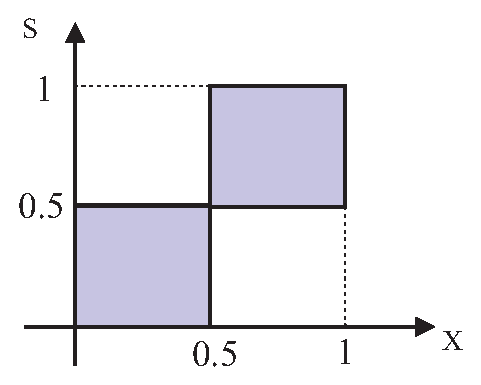
\epsfig{file=Figuras/graph_pxs,width=6cm}}
\vspace{.3cm}

Responda a las siguientes cuestiones justificando sus respuestas:

\begin{parts}
\part Si se sabe que $p_{X,S}(x,s)$ es constante en el dominio de definición, ¿cuál es el estimador MSE de $S$ a la vista de $X$? Represente gráficamente dicho estimador.
\part ¿Existe alguna $p_{X,S}(x,s)$ con el dominio anterior para la cual el estimador MSE de $S$ a la vista de $X$ sea $\widehat S_{\text{MSE}} = X/2$?
\part Justifique si existe alguna $p_{X,S}(x,s)$ con el dominio anterior tal que $\widehat S = 0.5$ sea:
\begin{itemize}
\item El estimador de mínimo error cuadrático de $S$ a la vista de $X$.
\item El estimador de mínimo error absoluto de $S$ a la vista de $X$.
\item El estimador de máximo a posteriori de $S$ a la vista de $X$.
\end{itemize}
\end{parts}

\begin{solution}
  \begin{parts}
\part $\widehat S_{\text{MSE}} = 0.25$ si $0<x<0.5$ y $\widehat S_{\text{MSE}} = 0.75$ si $0.5<x<1$ 

\part Para $0.5<x<1$, $p _{S|X}(s|x)$ está definida entre $0.5<s<1$, por lo que $X/2$ no puede ser el valor medio de $p _{S|X}(s|x)$
  
 \part   $\widehat S = 0.5$ no puede ser ni la media ni la mediana de $p_{S|X}(s|x)$, pero puede ser su máximo.  Luego, $\widehat S = 0.5$  no puede ser ni $\widehat S_{\text{MSE}} $, ni  $\widehat S_{\text{MAD}} $, pero puede ser  $\widehat S_{\text{MAP}} $.
 \end{parts}
 \end{solution}

\else

\question 

In the plot below, the shaded region shows the domain of a joint distribution of $S$ and $X$, i.e., the set of points for which $p_{X,S}(x,s)\neq 0$.

\vspace{.3cm}
\centerline{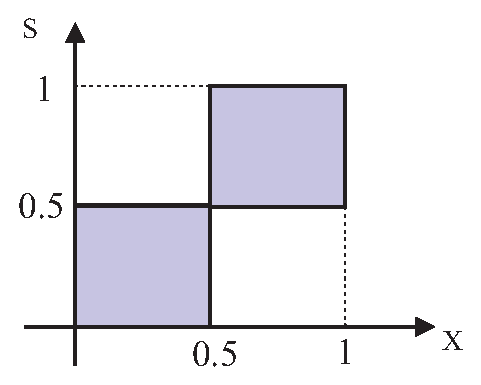
\epsfig{file=Figuras/graph_pxs,width=4cm}}
\vspace{.3cm}

Please, provide justified answers to the following questions:

\begin{parts}
\part If it is known that $p_{X,S}(x,s)$ is constant in its domain, which is the MSE estimator of $S$ given $X$? Provide a graphical representation of this estimator.
\part Is there any $p_{X,S}(x,s)$ with the previous domain for which the MSE estimator of $S$ given $X$ is $\SMSE = X/2$?
\part Justify if there exists any $p_{X,S}(x,s)$ with the previous domain, so that $\hat S = 0.5$ is:
\begin{itemize}
\item The minimum mean square error estimator of $S$ given $X$.
\item The minimum mean absolute deviation estimator of $S$ given $X$.
\item The maximum {\em a posteriori} estimator of $S$ given $X$.
\end{itemize}
\end{parts}

\begin{solution}
  \begin{parts}
\part $\SMSE = 0.25$ for $0<x<0.5$ and $\SMSE = 0.75$ for $0.5<x<1$ 

\part When $0.5<x<1$, $p _{S|X}(s|x)$ is non-zero for $0.5<s<1$, thus $X/2$ can never be the mean of $p _{S|X}(s|x)$ for that range of $X$.
  
\part $\hat S = 0.5$ cannot be the mean or the median of $p_{S|X}(s|x)$, but it can be its maximum.  Therefore, $\hat S = 0.5$  can just be  $\SMAP$ (but not  $\SMSE$ or $\SMAD$).
 \end{parts}
 \end{solution}

\fi

%%%%%%%%%%%%%%%%%%%%%%%%%%%%%%%%%%%%%%%%%%%%%%%%%%%%%%%%%%%%%%%
% Examen TDI Junio 2010 P3
\qformat{\textbf{\ej \thequestion ~~ (1.3; 1.4)} ~~ \linefill}
\ifspanish

\question 
La variable aleatoria $S$ sigue una distribución exponencial
\[
p_{S}(s) = \lambda e^{-\lambda s}, \qquad s>0
\]
siendo $\lambda>0$. La variable aleatoria discreta $X$ está relacionada con $S$ mediante una distribución de Poisson, es decir
\[
P_{X|S}(x|s) = \frac{s^x e^{-s}}{x!}, \qquad x=0,1,2,\ldots
\]

\begin{parts}
\part Determine el estimador ML de $S$ a la vista de $x$
\part Suponga que se observan $K$ realizaciones independientes $\{(x^{(k)},s^{(k)}),k=1,\ldots,K\}$ de $(X,S)$. Determine el estimador ML de $\lambda$ basado en ellas.
%\part Determine $p_{S|X}(s|1)$.
\part Determine el estimador MAP de $S$ a la vista de $x=1$.
\end{parts}

\begin{solution}
  \begin{parts}
\part $\widehat S_{\text{ML}} =X$ 
\part $\displaystyle \widehat \lambda_{\text{ML}} =\frac{1}{\frac{1}{K}\sum_{k=1}^K s^{(k)} }$ 
 \part  $\displaystyle \widehat S_{\text{MAP}} =\frac{X}{1+\lambda}$ 
 \end{parts}
 \end{solution}

\else

\question 
A random variable $S$ follows an exponential pdf
\[
p_{S}(s) = \lambda e^{-\lambda s}, \qquad s>0
\]
with $\lambda>0$. Consider now a discrete random variable $X$ related to $S$ via a Poisson distribution, i.e.,
\[
P_{X|S}(x|s) = \frac{s^x e^{-s}}{x!}, \qquad x=0,1,2,\ldots
\]

\begin{parts}
\part Determine the ML estimator of $S$ given $x$.
\part Assume now that we have access to $K$ independent realizations $\{(x^{(k)},s^{(k)}),k=1,\ldots,K\}$ of $(X,S)$. Find the ML estimator of $\lambda$ based on these observations.
%\part Determine $p_{S|X}(s|1)$.
\part Find the MAP estimation of $S$ for $x=1$.
\end{parts}

\begin{solution}
  \begin{parts}
\part $\widehat S_{\text{ML}} =X$ 
\part $\displaystyle \widehat \lambda_{\text{ML}} =\frac{1}{\frac{1}{K}\sum_{k=1}^K s^{(k)} }$ 
 \part  $\displaystyle \widehat S_{\text{MAP}} =\frac{X}{1+\lambda}$ 
 \end{parts}
 \end{solution}

\fi

%%%%%%%%%%%%%%%%%%%%%%%%%%%%%%%%%%%%%%%%%%%%%%%%%%%%%%%%%%%%%%%%
%% Examen TDI Mayo 2011 P2
\qformat{\textbf{\ej \thequestion ~~ (1.5; 1.7)} ~~ \linefill}
\ifspanish

\question 
 Se desea estimar la v.a. $S$ a partir de la observación $X$ dada por:

$$X=S+N_1+N_2$$

donde $S$ es una v.a. gaussiana de media $m_s$ y varianza $v_s$, y donde $N_1$ y $N_2$ son dos variables de ruido, independientes de $S$, cuya d.d.p. conjunta viene dada por:
 $$p_{N_1,N_2}\left ( n_1,n_2\right) \sim G\left (  \left[ \begin{array}{c}   0 \\ 0    \end{array} \right] , \left[ \begin{array}{cc}  v_1 & v_{12} \\ v_{12} & v_2  \end{array} \right]\right)$$

Obtenga:
\begin{parts}
\part El estimador de mínimo error cuadrático medio de $S$ a la vista de $X$, $\widehat S_{\text{MMSE}}$.
\part El estimador de máximo a posteriori de $S$ a la vista de $X$, $\widehat S_{\text{MAP}}$.
\part Calcule el sesgo y varianza de ambos estimadores. 
\end{parts}

\begin{solution}
  \begin{parts}
  \part $\displaystyle \widehat S_{\text{MMSE}}=\frac{v_s}{v_s+v_1+v_2+2v_{12}}X+m_s\left( 1-\frac{v_s}{v_s+v_1+v_2+2v_{12}}\right) $
  \part $\widehat S_{\text{MAP}}= \widehat S_{\text{MMSE}}$
  \part $\EE\left\{\widehat S_{\text{MMSE}} - S \right\} = \quad 
         \EE\left\{\widehat S_{\text{MAP}}  - S \right\} = 0$ \\
  $ \displaystyle {\rm Var} \left\lbrace  \widehat S_{\text{MMSE}} \right\rbrace = {\rm Var} \left\lbrace  \widehat S_{\text{MAP}}  \right\rbrace = {\frac{v_s^2}{v_s+v_1+v_2+2v_{12}}}$
 \end{parts}
 \end{solution}

\else

\question 
 We wish to estimate a random variable $S$ from the observation of another random variable $X$ given by:

$$X=S+N_1+N_2$$

where $S$ is Gaussian-distributed, with mean and variance $m_s$ and $v_s$, respectively, and where $N_1$ and $N_2$ are two noise random variables, independent of $S$, and with joint p.d.f. 
 $$p_{N_1,N_2}\left ( n_1,n_2\right) \sim G\left (  \left[ \begin{array}{c}   0 \\ 0    \end{array} \right] , \left[ \begin{array}{cc}  v_1 & v_{12} \\ v_{12} & v_2  \end{array} \right]\right)$$

Obtain:
\begin{parts}
\part The minimum mean square error estimator of $S$ given $X$, $\widehat S_{\text{MMSE}}$.
\part The maximum a posteriori estimator of $S$ given $X$, $\widehat S_{\text{MAP}}$.
\part The bias and variance of both estimators. 
\end{parts}

\begin{solution}
  \begin{parts}
 \part  $\displaystyle \widehat S_{\text{MMSE}}=\frac{v_s}{v_s+v_1+v_2+2v_{12}}X+m_s\left( 1-\frac{v_s}{v_s+v_1+v_2+2v_{12}}\right) $
  \part $\widehat S_{\text{MAP}}= \widehat S_{\text{MMSE}}$
  \part $\EE\left\{\widehat S_{\text{MMSE}} - S \right\} = \quad 
         \EE\left\{\widehat S_{\text{MAP}}  - S \right\} = 0$ \\
  $ \displaystyle {\rm Var} \left\lbrace  \widehat S_{\text{MMSE}}  \right\rbrace= {\rm Var} \left\lbrace  \widehat S_{\text{MAP}}  \right\rbrace=  \frac{v_s^2}{v_s+v_1+v_2+2v_{12}}$
 \end{parts}
 \end{solution}

\fi

%%%%%%%%%%%%%%%%%%%%%%%%%%%%%%%%%%%%%%%%%%%%%%%%%%%%%%%%%%%%%%%%
%% Examen TDI Mayo 2011 P4
\qformat{\textbf{\ej \thequestion ~~ (1.4; 1.7)} ~~ \linefill}
\ifspanish

\question Se dispone de una colección de observaciones $\{x_k, k=0,\ldots,K-1\}$ independientes con distribución de Pareto de parámetros deterministas $\alpha$ y $\beta$, es decir,
\[
p_{X|\alpha,\beta}(x|\alpha,\beta) = \frac{\alpha \beta^{\alpha}}{x^{\alpha+1}},  \qquad  x \ge \beta
\]
siendo $\alpha>1$ y $\beta>0$.
\begin{parts}
\part Supuesto conocido $\beta$, determine el estimador ML de $\alpha$, $\hat{\alpha}_{\text{ML}}$. 
\part Suponiendo $K=1$ (es decir, una sola observación), determine el estimador ML de $\beta$, $\hat{\beta}_{\text{ML}}$. 
\part Suponiendo $K=1$, determine el sesgo de $\widehat{\beta}_{\text{ML}}$.
\end{parts}
\begin{solution}
\begin{parts}
\part $\hat{\alpha}_{\text{ML}}=\frac{K}{\sum_{k=0}^{K-1}  \ln {\frac{x_k}{\beta}} }$
\part $\hat{\beta}_{\text{ML}}=x_0$
\part ${\rm bias}\left\{ \hat{\beta}_{\text{ML}} | \beta \right\} =  \frac{1}{\alpha-1} \beta$
\end{parts}
\end{solution}

\else

\question We have access to a set of observations $\{x_k, k=0,\ldots,K-1\}$, independently drawn from a Pareto distribution with deterministic parameters $\alpha$ and $\beta$, i.e.,
\[
p_{X|\alpha,\beta}(x|\alpha,\beta) = \frac{\alpha \beta^{\alpha}}{x^{\alpha+1}},  \qquad  x \ge \beta
\]
with $\alpha>1$ and $\beta>0$.
\begin{parts}
\part Assuming that $\beta$ is known, find the ML estimator of $\alpha$, $\hat{\alpha}_{\text{ML}}$. 
\part For $K=1$ (i.e., just one observation), find the ML estimator of $\beta$, $\hat{\beta}_{\text{ML}}$. 
\part For $K=1$, compute the bias of $\hat{\beta}_{\text{ML}}$.
\end{parts}

\begin{solution}
\begin{parts}
\part $\hat{\alpha}_{\text{ML}}=\frac{K}{\sum_{k=0}^{K-1}  \ln {\frac{x_k}{\beta}} }$
\part $\hat{\beta}_{\text{ML}}=x_0$
\part ${\rm bias}\left\{ \hat{\beta}_{\text{ML}} | \beta \right\} =  \frac{1}{\alpha-1} \beta$
\end{parts}
\end{solution}

\fi
 
%%%%%%%%%%%%%%%%%%%%%%%%%%%%%%%%%%%%%%%%%%%%%%%%%%%%%%%%%%%%%%%%
%% Examen TDI Junio 2011 P1
\qformat{\textbf{\ej \thequestion ~~ (1.3)} ~~ \linefill}
\ifspanish

\question  Construya el estimador de mínimo error cuadrático medio de la variable aleatoria $S$ a partir de la observación de una variable aleatoria $X$ en los siguientes casos:

\begin{parts}
\part 
\[
p_{X,S}(x,s) = \left \{
  \begin{array}{cc}
    1, &
         0 \le x \le 1, ~~ \quad 0\le s \le 1 \\
0,  & \mbox{en el resto}
  \end{array}
\right.
\]
  \part 

\[
p_{X,S}(x,s) = \left \{
  \begin{array}{cc}
    2, &  0 \leq s \leq 1-x, ~~ 0 \leq x \leq 1 \\
0, & \mbox{en el resto}
  \end{array}
\right.
\]

\end{parts}
 
\begin{solution}
  \begin{parts}
 \part  $\widehat S_{\text{MMSE}}=\frac{1}{2}$
 \part  $\widehat S_{\text{MMSE}}=\frac{1-X}{2}$
 \end{parts}

 \end{solution}

\else

\question  Obtain the minimum mean square error estimator of random variable $S$ based on the observation of random variable $X$, in the following two cases:

\begin{parts}

\part 
\[
p_{X,S}(x,s) = \left \{
  \begin{array}{cc}
    1, &
         0 \le x \le 1, ~~ \quad 0\le s \le 1 \\
0,  & \mbox{otherwise}
  \end{array}
\right.
\]

\part 
\[
p_{X,S}(x,s) = \left \{
  \begin{array}{cc}
    2, &  0 \leq s \leq 1-x, ~~ 0 \leq x \leq 1 \\
0, & \mbox{otherwise}
  \end{array}
\right.
\]
\end{parts}

 
\begin{solution}
  \begin{parts}
 \part  $\widehat S_{\text{MMSE}}=\frac{1}{2}$
 \part  $\widehat S_{\text{MMSE}}=\frac{1-X}{2}$
 \end{parts}

 \end{solution}

\fi
 
%%%%%%%%%%%%%%%%%%%%%%%%%%%%%%%%%%%%%%%%%%%%%%%%%%%%%%%%%%%%%%%%
%% Examen TDI Junio 2011 P4
\qformat{\textbf{\ej \thequestion ~~ (1.3; 1.7)} ~~ \linefill}
\ifspanish

\question  Se desea estimar la v.a. $S$ a partir de la observación $X$ y para ello se conoce la distribución conjunta de ambas:

$$p_{S,X}(s,x)= \left\lbrace  \begin{array}{ll} 6s, & 0<s<x-1, \; \; 1<x<2 \\
0, & \mbox{en el resto}  \end{array}  \right. $$

 Obtenga:
\begin{parts}
\part El estimador de mínimo error cuadrático medio de $S$ a la vista de $X$, $\widehat S_{\text{MMSE}}$.
\part El estimador de máximo a posteriori de $S$ a la vista de $X$, $\widehat S_{\text{MAP}}$.
\part El estimador de mínimo error absoluto de $S$ a la vista de $X$, $\widehat S_{\text{MAD}}$.
\part Calcule el sesgo de los estimadores anteriores. 
\end{parts}

 \begin{solution}
 
 Una resolucion en vídeo de este problema puede encontrarse en
 
\url{http://decisionyestimacion.blogspot.com/2013/05/p37-estimacion.html}

\begin{parts}
 \part $\widehat S_{\text{MMSE}}=\frac{2}{3}\left(X-1 \right) $
 \part $\widehat S_{\text{MAP}}=X-1 $
 \part $\widehat S_{\text{MAD}}=\frac{1}{\sqrt{2}}\left(X-1 \right)  $
 \part $\mathbb E \left\lbrace S- \widehat S_{\text{MMSE}}  \right\rbrace =0  \quad  \mathbb E \left\lbrace S- \widehat S_{\text{MAP}}  \right\rbrace =-0.25  \quad \mathbb E \left\lbrace S- \widehat S_{\text{MAD}}  \right\rbrace =-0.03 $
\end{parts}
\end{solution}

\else

\question Consider the estimation of a random variable $S$ based on the observation of $X$, where the two variables satisfy the following joint pdf:

$$p_{S,X}(s,x)= \left\lbrace  \begin{array}{ll} 6s, & 0<s<x-1, \; \; 1<x<2 \\
0, & \mbox{otherwise}  \end{array}  \right. $$

Obtain:
\begin{parts}
\part The minimum mean square error estimator of $S$ given $X$, $\widehat S_{\text{MMSE}}$.
\part The maximum {\em a posteriori} estimator of $S$ given $X$, $\widehat S_{\text{MAP}}$.
\part The minimum mean absolute error estimator of $S$ given $X$, $\widehat S_{\text{MAD}}$.
\part The bias of all previous estimators. 
\end{parts}

 \begin{solution}
 
 A video resolution of this problem (in Spanish) can be found in
 
\url{http://decisionyestimacion.blogspot.com/2013/05/p37-estimacion.html}

\begin{parts}
 \part   $\widehat S_{\text{MMSE}}=\frac{2}{3}\left(X-1 \right) $
  \part   $\widehat S_{\text{MAP}}=X-1 $
  \part   $\widehat S_{\text{MAD}}=\frac{1}{\sqrt{2}}\left(X-1 \right)  $
 \part   $\mathbb E \left\lbrace S- \widehat S_{\text{MMSE}}  \right\rbrace =0  \quad  \mathbb E \left\lbrace S- \widehat S_{\text{MAP}}  \right\rbrace =-0.25  \quad \mathbb E \left\lbrace S- \widehat S_{\text{MAD}}  \right\rbrace =-0.03 $
  
 \end{parts}
 \end{solution}

\fi
%
%%%%%%%%%%%%%%%%%%%%%%%%%%%%%%%%%%%%%%%%%%%%%%%%%%%%%%%%%%%%%%%%
%%%%%%%%%%%%%% Enero 2012: Estimación ML parametro determinista
\qformat{\textbf{\ej \thequestion ~~ (1.4; 1.7)} ~~ \linefill}
\ifspanish

\question Se dispone de una colección de observaciones $\{x^{(k)}, k=1,\ldots,K\}$ independientes con distribución de Rayleigh de parámetro $b$, es decir,
\[
p_{X|b}(x|b) = \frac{2}{b} x \exp \left( -\frac{x^2}{b}\right) ,  \qquad  x \ge 0
\]
siendo $b>0$.

\begin{parts}
\part Determine el estimador ML de $b$, $\widehat{b}_{\text{ML}}$. 
\part Si el conjunto de valores observados es $\{2, 0, 1, 1\}$, ¿cuál sería el valor más verosímil del parámetro $b$?
\part Determine el sesgo del estimador. 
\end{parts}


\begin{solution}
\begin{parts}
\part $\widehat{b}_{\text{ML}}=\displaystyle \frac{1}{K} \sum_{k=1}^K \left( x^{(k)}\right) ^2 $
\part $\widehat{b}_{\text{ML}}=1.5$
\part Insesgado
\end{parts}
\end{solution}

\else

\question We have access to a collection of observations $\{x^{(k)}, k=1,\ldots,K\}$ independently drawn from a Rayleigh distribution with parameter $b$, i.e.,
\[
p_{X|b}(x|b) = \frac{2}{b} x \exp \left( -\frac{x^2}{b}\right) ,  \qquad  x \ge 0
\]
with $b>0$.

\begin{parts}
\part Determine the ML estimator of $b$, $\widehat{b}_{\text{ML}}$. 
\part If the observations are $\{2, 0, 1, 1\}$, what would be the most likelihood value of  $b$?
\part Find the bias of the estimator. 
\end{parts}


\begin{solution}
\begin{parts}
\part $\widehat{b}_{\text{ML}}=\displaystyle \frac{1}{K} \sum_{k=1}^K \left( x^{(k)}\right) ^2 $
\part $\widehat{b}_{\text{ML}}=1.5$
\part The estimator is unbiased.
\end{parts}
\end{solution}

\fi
%
%%%%%%%%%%%%%%%%%%%%%%%%%%%%%%%%%%%%%%%%%%%%%%%%%%%%%%%%%%%%%%%%
%%%%%%%%%%%%%% Enero 2012: Estimación de variable aleatoria.
\qformat{\textbf{\ej \thequestion ~~ (1.3; 1.7)} ~~ \linefill}
\ifspanish

\question Se dispone de tres variables aleatorias independientes $S_1$, $S_2$ y $S_3$, con idéntica fdp a priori. A partir de una observación de $X = S_1 + S_2 + S_3$ se desea estimar $S_1$. 

\begin{parts}
\part Justifique brevemente por qué el estimador de mínimo error cuadrático de $S_1$ dado $x$ es $\displaystyle \hat{s}_1 = \frac{x}{3}$.
\part Calcule el sesgo de dicho estimador. ¿Es sesgado o insesgado?
\vspace{0.4cm}

\hspace{-0.8 cm} Asumiendo en los apartados siguientes que $S_1$, $S_2$ y $S_3$ tienen una fdp uniforme entre -1 y 1:

\part Calcule la fdp de $X$ dado $s_1$.
\part Calcule la varianza del estimador $\hat{S}_1$.
\end{parts}

\begin{solution}
\begin{parts}
\part Por la simetría del problema, todas las $\mathbb{E}\{S_i|x\}$ deben ser iguales y sumar $x$.
\part 0, insesgado.
\part $p_{X|S_1}(x|s_1) = 1/2- |x-s_1|/4$ para $-2 < x < 2$, 0 en otro caso.
\part $1/9$
\end{parts}
\end{solution}

\else

\question Consider three independent random variables, $S_1$, $S_2$ and $S_3$, with the same {\em a priori} pdf. We wish to estimate $S_1$ from a single observation of $X = S_1 + S_2 + S_3$. 

\begin{parts}
\part Justify briefly why the minimum mean square error estimator of $S_1$ given $x$ is $\hat{s}_1 = \dfrac{x}{3}$.
\part Find the bias of the estimator given in (a).  Is it biased or unbiased?
\vspace{0.4cm}

\hspace{-0.8 cm} Assuming in the following that $S_1$, $S_2$ and $S_3$ follow a uniform distribution between $-1$ and $1$:

\part Obtain the pdf of $X$ given $s_1$.
\part Find the variance of estimator $\hat{S}_1$.
\end{parts}

\begin{solution}
\begin{parts}
\part Using symmetry arguments, all $\EE\{S_i|x\}$ should be the same and sum up to $x$.
\part The estimator is unbiased.
\part $p_{X|S_1}(x|s_1) = 1/2- |x-s_1|/4$ for $-2 < x < 2$, and $0$ otherwise.
\part $\text{var}(S_1) = 1/9$
\end{parts}
\end{solution}

\fi
%
%%%%%%%%%%%%%%%%%%%%%%%%%%%%%%%%%%%%%%%%%%%%%%%%%%%%%%%%%%%%%%%%
%%%%%%%%%%%%%% JUNIO 2012: Estimación gauss
\qformat{\textbf{\ej \thequestion ~~ (1.5)} ~~ \linefill}
\ifspanish

\question Dos variables aleatorias Gaussianas independientes $Z_1$ y $Z_2$ tienen medias 2 y 1, respectivamente. Ambas tienen varianza unidad. Estamos interesados en su diferencia $S = Z_1 - Z_2$.

\begin{parts}
\part Calcule $p_S(s)$, el estimador MMSE de $S$ y el error cuadrático medio de dicho estimador, si no se dispone de ningún dato adicional.
\part A continuación se observa $X = Z_1 + Z_2 = 3$. Calcule $p_{S|X}(s|x)$, el estimador MMSE de $S$ a la vista de $X$ y el error cuadrático medio de dicho estimador. Interprete el resultado obtenido en relación con el apartado anterior.
\end{parts}

\begin{solution}
\begin{parts}
\part $\widehat S_{\text{MMSE}} = 1$, con varianza $2$.
\part $X$ es independiente de $S$, por lo que la respuesta es la misma que en a).
\end{parts}
\end{solution}

\else

\question Two independent Gaussian variables $Z_1$ and $Z_2$ have means 2 and 1, respectively. Both variables have unit variance. We wish to estimate the difference $S = Z_1 - Z_2$.

\begin{parts}
\part Obtain $p_S(s)$, the MMSE estimator of $S$, and the mean square error of such estimator if no other information is available.
\part Consider now we can observe $X = Z_1 + Z_2 = 3$. Find $p_{S|X}(s|x)$, the MMSE estimator of $S$ given $X$, and the mean square error of such estimator. Discuss your result in relation to your answers to the previous subsection.
\end{parts}

\begin{solution}
\begin{parts}
\part $\widehat S_{\text{MMSE}} = 1$;  $\mathbb E\left\{\left(S - \widehat S_{\text{MMSE}}\right)^2\right\} = 2$.
\part $X$ is independent of $S$, thus the answers are the same as in subsection (a).
\end{parts}
\end{solution}

\fi
%
%%%%%%%%%%%%%%%%%%%%%%%%%%%%%%%%%%%%%%%%%%%%%%%%%%%%%%%%%%%%%%%%
%%%%%%%%%%%%%% JUNIO 2012: Estimación gral
\qformat{\textbf{\ej \thequestion ~~ (1.2;1.3)} ~~ \linefill}
\ifspanish

\question[25] Se desea estimar la variable aleatoria $S$ a partir de la variable aleatoria $X$ conociendo la función de densidad de probabilidad conjunta de ambas, dada por:
 
 $$p_{S,X}(s,x)=24 xs, \quad 0 \leq s \leq 1-x, \; 0<x<1   $$
 
 \begin{parts}
\part Calcule el estimador de mínimo error cuadrático medio de $S$ a la vista de $X$, $\SMSE$.
\part Calcule el estimador MAP de $S$ a la vista de $X$, $\SMAP$.
\part Calcule el estimador MAD de $S$ a la vista de $X$, $\SMAD$.
\part El estimador de la forma  $\hat{S}_\text{CUAD}=w X^2$ de mínimo error cuadrático medio.
\end{parts}

\begin{solution}
\begin{parts}
\part $\hat{S}_\text{MMSE}=\displaystyle\frac{2}{3} \left( 1-X \right)$.
\part Dado que $p_{S|X}(s|x)$ es creciente con $s$, $\hat{S}_\text{MAP}=1-X$.
\part $\hat{S}_\text{MAD}=\displaystyle \frac{1-X}{\sqrt{2}}$.
\part $w = 0.8$
\end{parts}
\end{solution}

\else

\question We wish to estimate a random variable $S$ based on the observation of $X$. Their joint pdf is given by:
 
 $$p_{S,X}(s,x)=24 xs, \quad 0 \leq s \leq 1-x, \; 0<x<1   $$
 
 
Find: 
 \begin{parts}
\part The minimum mean square error estimator of $S$ given $X$, $\SMSE$.
\part The MAP estimator of $S$ given $X$, $\SMAP$.
\part The MAD estimator of $S$ given $X$, $\SMAD$.
\part The estimator in the form $\hat{S}_\text{q}=w X^2$ that minimizes the mean square error.
\end{parts}

\begin{solution}
\begin{parts}
\part $\SMSE = \dfrac{2}{3} \left( 1-X \right)$.
\part Since $p_{S|X}(s|x)$ is strictly increasing with respect to $s$, $\SMAP=1-X$.
\part $\SMAD=\dfrac{1-X}{\sqrt{2}}$.
\part $w = 0.8$
\end{parts}
\end{solution}

\fi

%%%%%%%%%%%%%%%%%%%%%%%%%%%%%%%%%%%%%%%%%%%%%%%%%%%%%%%%%%%%%%%
%%%%%%%%%%%%%% ENERO 2013: Estimación lineal MSE
\qformat{\textbf{\ej \thequestion ~~ (LMSE)} ~~ \linefill}
\ifspanish

\question[20] 

Se sabe que la distribución conjunta de $S$ con $X$ viene dada por:
$$p_{S,X}(s,x) = \frac{1}{3} \left( x+s\right) \quad 0<x<2, ~~0<s<1.  $$

\begin{parts}
\part Obtenga el estimador lineal de mínimo error cuadrático medio, $\hat{S}_{\rm LMSE}=w_0+w_1 X$.
\part Calcule el error cuadrático medio del estimador.
\end{parts}

\begin{solution}
\begin{parts}
\part $\displaystyle \hat{s}_{\rm LMSE}=\frac{14}{23}- \frac{1}{23} x$.
\part $\displaystyle \mathbb{E} \left\lbrace \left( S- \hat{S}_{\rm LMSE}\right) ^2\right\rbrace =\frac{11}{138}$
\end{parts}
\end{solution}

\else

\question The joint pdf of two random variables $S$ and $X$ is given by:
$$p_{S,X}(s,x) = \frac{1}{3} \left( x+s\right) \quad 0<x<2, ~~0<s<1.  $$
\begin{parts}
\part Obtain the Linear Minimum Mean Square Error estimator, $\widehat{S}_{\rm LMSE}=w_0+w_1 X$.
\part Calculate the mean square error of the estimator.
\end{parts}

%Se sabe que la distribución conjunta de $S$ con $X$ viene dada por:
%$$p_{S,X}(s,x) = \frac{1}{3} \left( x+s\right) \quad 0<x<2, ~~0<s<1.  $$
%
%\begin{parts}
%\part Obtenga el estimador lineal de mínimo error cuadrático medio, $\hat{S}_{\rm LMSE}=w_0+w_1 X$.
%\part Calcule el error cuadrático medio del estimador.
%\end{parts}

\begin{solution}
\begin{parts}
\part $\displaystyle \hat{s}_{\rm LMSE}=\frac{14}{23}- \frac{1}{23} x$.
\part $\displaystyle \mathbb{E} \left\lbrace \left( S- \hat{S}_{\rm LMSE}\right) ^2\right\rbrace =\frac{11}{138}$
\end{parts}
\end{solution}

\fi
%
%%%%%%%%%%%%%%%%%%%%%%%%%%%%%%%%%%%%%%%%%%%%%%%%%%%%%%%%%%%%%%%%
%%%%%%%%%%%%%% ENERO 2013:  
\qformat{\textbf{\ej \thequestion ~~ (ML, MSE)} ~~ \linefill}
\ifspanish

\question[25] % VGV

El encargado de una empresa informática desea analizar la productividad de sus empleados mediante la estimación del tiempo, $S$, que les lleva desarrollar cierto programa informático. Para ello, a las 12:00 a.m. el encargado solicita a sus empleados la realización de este programa. Los empleados no atienden la petición hasta que finalicen la tarea que estén llevando a cabo en ese momento, lo que les lleva un tiempo adicional $N$. En consecuencia, el tiempo total transcurrido desde la petición del encargado hasta que el empleado termina el programa es $X=S+N$.

Se sabe que el tiempo $N$ puede modelarse mediante la siguiente distribución exponencial:
$$p_{N}(n) = a \exp \left(-a n \right)  \quad n>0,$$ mientras que $S$ puede modelarse mediante una exponencial retardada, es decir:
$$p_{S}(s) = b \exp \left(-b  \left(s-c \right)    \right)  \quad s>c.$$

\begin{parts}
\part Antes de iniciar el análisis de productividad sobre los empleados, se ha simulado sobre un grupo de control, midiendo directamente sobre este grupo los tiempos que han tardado en acabar las tareas que están realizando y los tiempos que han tardado en desarrollar el programa informático. Como consecuencia se tienen los siguientes conjuntos de observaciones independientes: $6$, $10$, $12$ y $20$ minutos  para el tiempo $N$ y $6$, $12$, $18$ y $36$ minutos para el tiempo $S$. Estime por máxima verosimilitud los valores de las constantes $a$, $b$ y $c$.
\end{parts}
Considere de ahora en adelante que $a=10$ minutos, $b=10$ minutos y $c=5$ minutos.
\begin{parts}
\addtocounter{partno}{1} 
\part Si cuando comienza el análisis de productividad, el encargado recibe la notificación de finalización del programa de tres empleados diferentes a las $12$:$25$, a las $12$:$30$ y a las $12$:$40$ a.m., estime por máxima verosimilitud el tiempo que ha tardado cada uno de estos empleados en realizar el programa.
\part ¿Qué tiempo estimaríamos que ha tardado cada uno de estos empleados si utilizásemos un estimador de mínimo error cuadrático medio?
\end{parts}

\else

\question The manager of an IT company intends to analyze the productivity of his employees by estimating the time $S$ they need to implement a certain computer program. With this goal, at 12:00 a.m. the manager requests the implementation of the program; instead of directly starting the coding task, the employees need to finish first whatever task they are currently carrying out, what requires an additional time $N$. As a consequence, the total elapsed time between the request of the program implementation and each employee's notification indicating the conclusion of the task is $X=S+N$.

It is known that the time $N$ that the employees need to finish the tasks and start the program implementation can be modeled as the following exponential distribution
$$p_{N}(n) = a \exp \left(-a n \right)  \quad n>0,$$
whereas the time for coding the program, $S$, follows also an exponential distribution, in this case characterized by the expression
$$p_{S}(s) = b \exp \left(-b  \left(s-c \right)    \right)  \quad s>c.$$

\begin{parts}
\part Before the described process, a simulation has been carried out using a control group, and measuring directly the times $N$ and $S$ required by the members of this group. As a result of the test, four independent observations were obtained for each variable. Concretely, the four observations for $N$ were $6$, $10$, $12$, and $20$ minutes, whereas the observations for $S$ were $6$, $12$, $18$, and $36$ minutes. Based on these observations, estimate using maximum likelihood the values of constants $a$, $b$, and $c$.
\end{parts}
Consider in the following $a=10$ minutes, $b=10$ minutes, and $c=5$ minutes.
\begin{parts}
\addtocounter{partno}{1} 
\part For the actual productivity test, the manager receives notifications from three different employees indicating that they have finished the implementation of the program at $12$:$25$, $12$:$30$, and $12$:$40$ a.m.  Estimate using maximum likelihood the time that each employee needed for the implementation of the program.
\part Repeat the estimation of the previous subsection if a minimum mean square error estimator were used.
\end{parts}

\fi

\begin{solution}
\begin{parts}
\part $\hat{a}_{\rm ML} = \frac{K}{\sum_{k=0}^{K-1} n_k}= \dfrac{1}{12}$ minutes$^{-1}$;\\
$\hat{c}_{\rm ML}= \min_k \left\{ s_k \right\} = 6$ minutes;\\ 
$\hat{b}_{\rm ML}= \frac{K}{\sum_{k=0}^{K-1} \left( s_k -\hat{c}_{\rm ML} \right)} = \dfrac{1}{12}$ minutes$^{-1}$.
\part $\sML=x$. $\sML(x=25)=25$, $\sML(x=30)=30$,$\sML(x=40)=40$.
\part $\sMSE = \frac{x+5}{2}$, $\sMSE(x=25)=15$, $\sMSE(x=30)=17.5$,$\sMSE(x=40)=22.5$.
\end{parts}
\end{solution}


%
%%%%%%%%%%%%%%%%%%%%%%%%%%%%%%%%%%%%%%%%%%%%%%%%%%%%%%%%%%%%%%%%
%%%%%%%%%%%%%% Cuestión II: JULIO 2013
\qformat{\textbf{\ej \thequestion ~~ (MSE, MAD)} ~~ \linefill}
\ifspanish

\question[20] 

Se sabe que la distribución conjunta de $S$ con $X$ viene dada por:
$$p_{S,X}(s,x) = \left[\begin{array}{ll}
  \frac{4s}{x(1-x)}, & x(1-x)<s<2x(1-x), \quad 0<x<1 \\
  0,                 & \text{resto}
\end{array}  
\right. 
$$

\begin{parts}
\part Represente, de forma aproximada, la región de soporte de la distribución conjunta.
\part Determine el estimador $\widehat S_{\text{MMSE}}$.
\part Determine el estimador $\widehat S_{\text{MAD}}$.
\end{parts}

\begin{solution}
\begin{parts}
\part La región de soporte es la zona sombreada de la figura

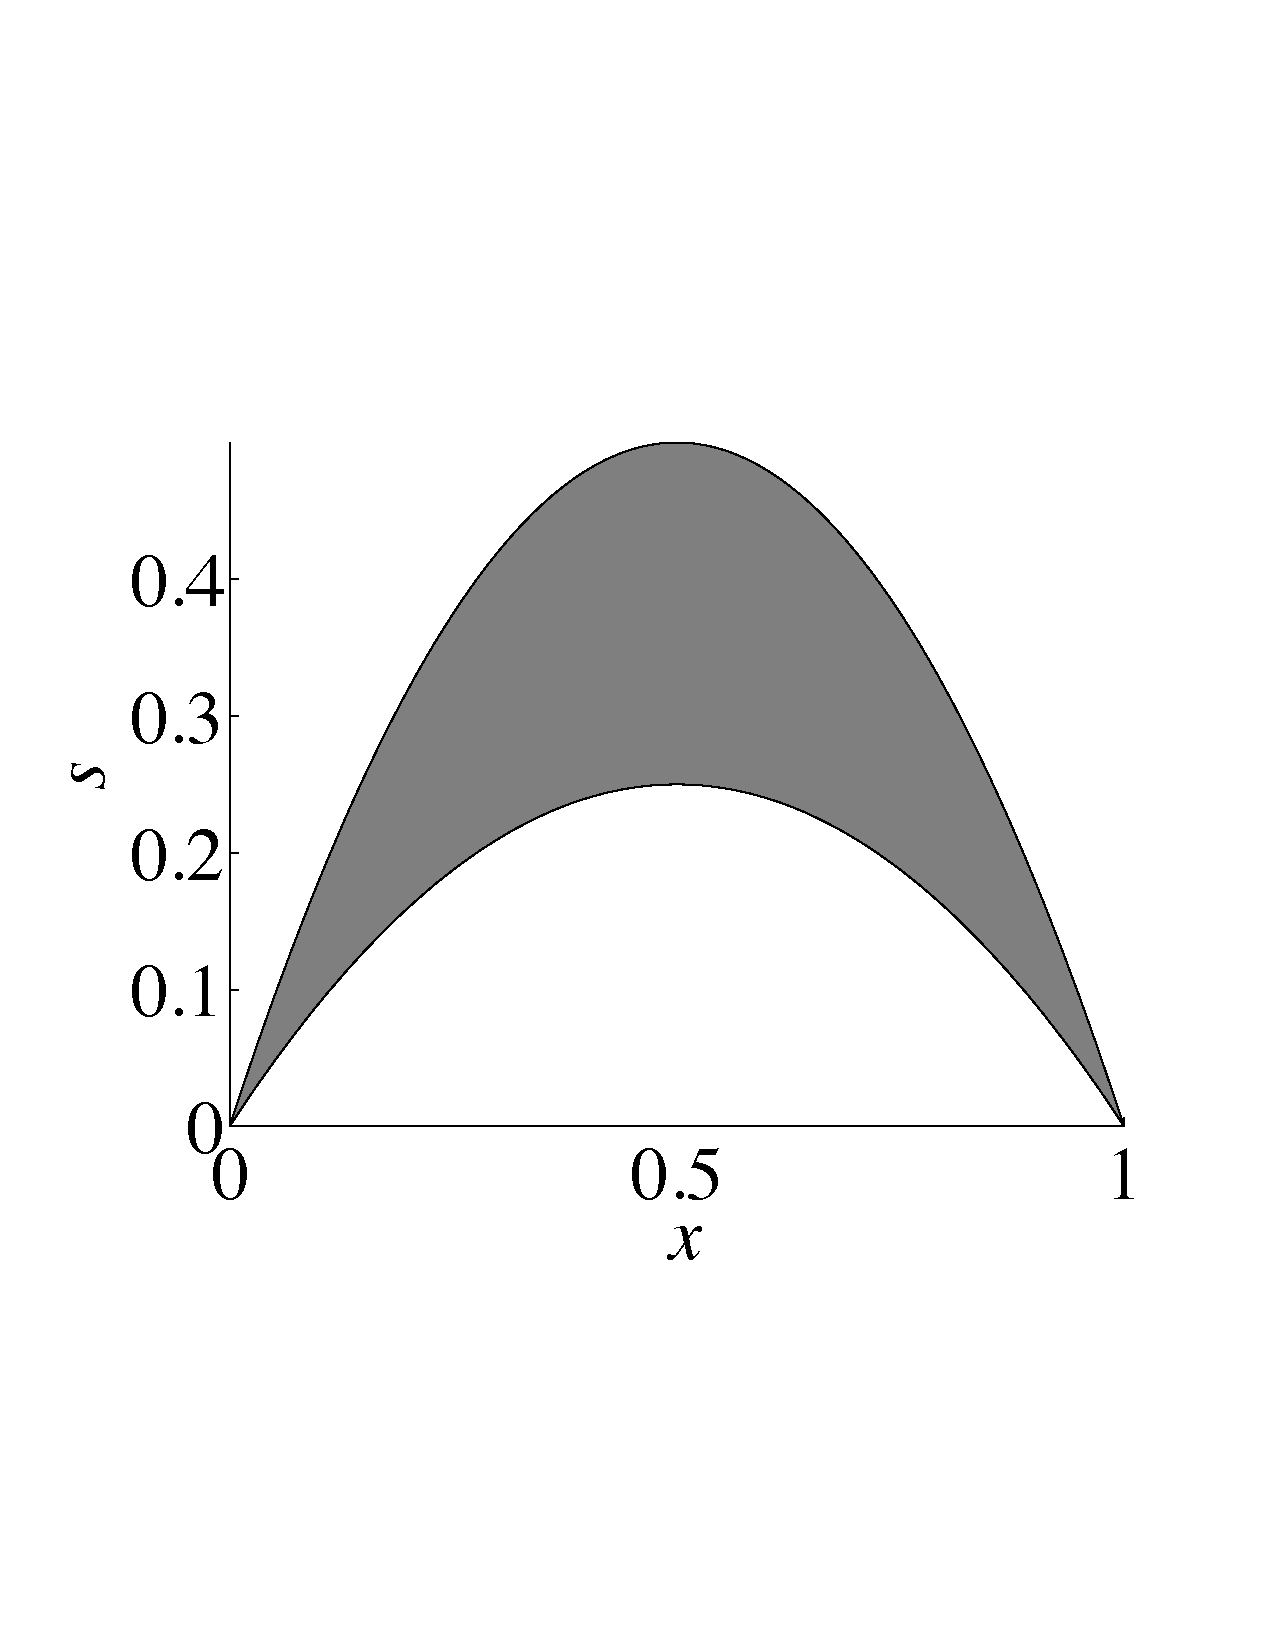
\includegraphics[width=3.5cm]{Figuras/RegionSoporteJun2013.pdf}
\part $\displaystyle \hat{s}_{\rm MMSE}= \frac{14}{9}x(1-x)$.
\part $\displaystyle \hat{s}_{\rm MAD} = \sqrt{\frac{5}{2}}x(1-x)$
\end{parts}
\end{solution}

\else

\question The joint pdf of two random variables $S$ and $X$ is given by:
$$p_{S,X}(s,x) = \frac{4s}{x(1-x)}, \qquad x(1-x)<s<2x(1-x), \qquad 0<x<1
$$

\begin{parts}
\part Provide an approximate representation of the support of the joint distribution.
\part Find $\SMSE$.
\part Find $\SMAD$.
\end{parts}

\begin{solution}
\begin{parts}
\part The support of the pdf is the shaded region in the figure:

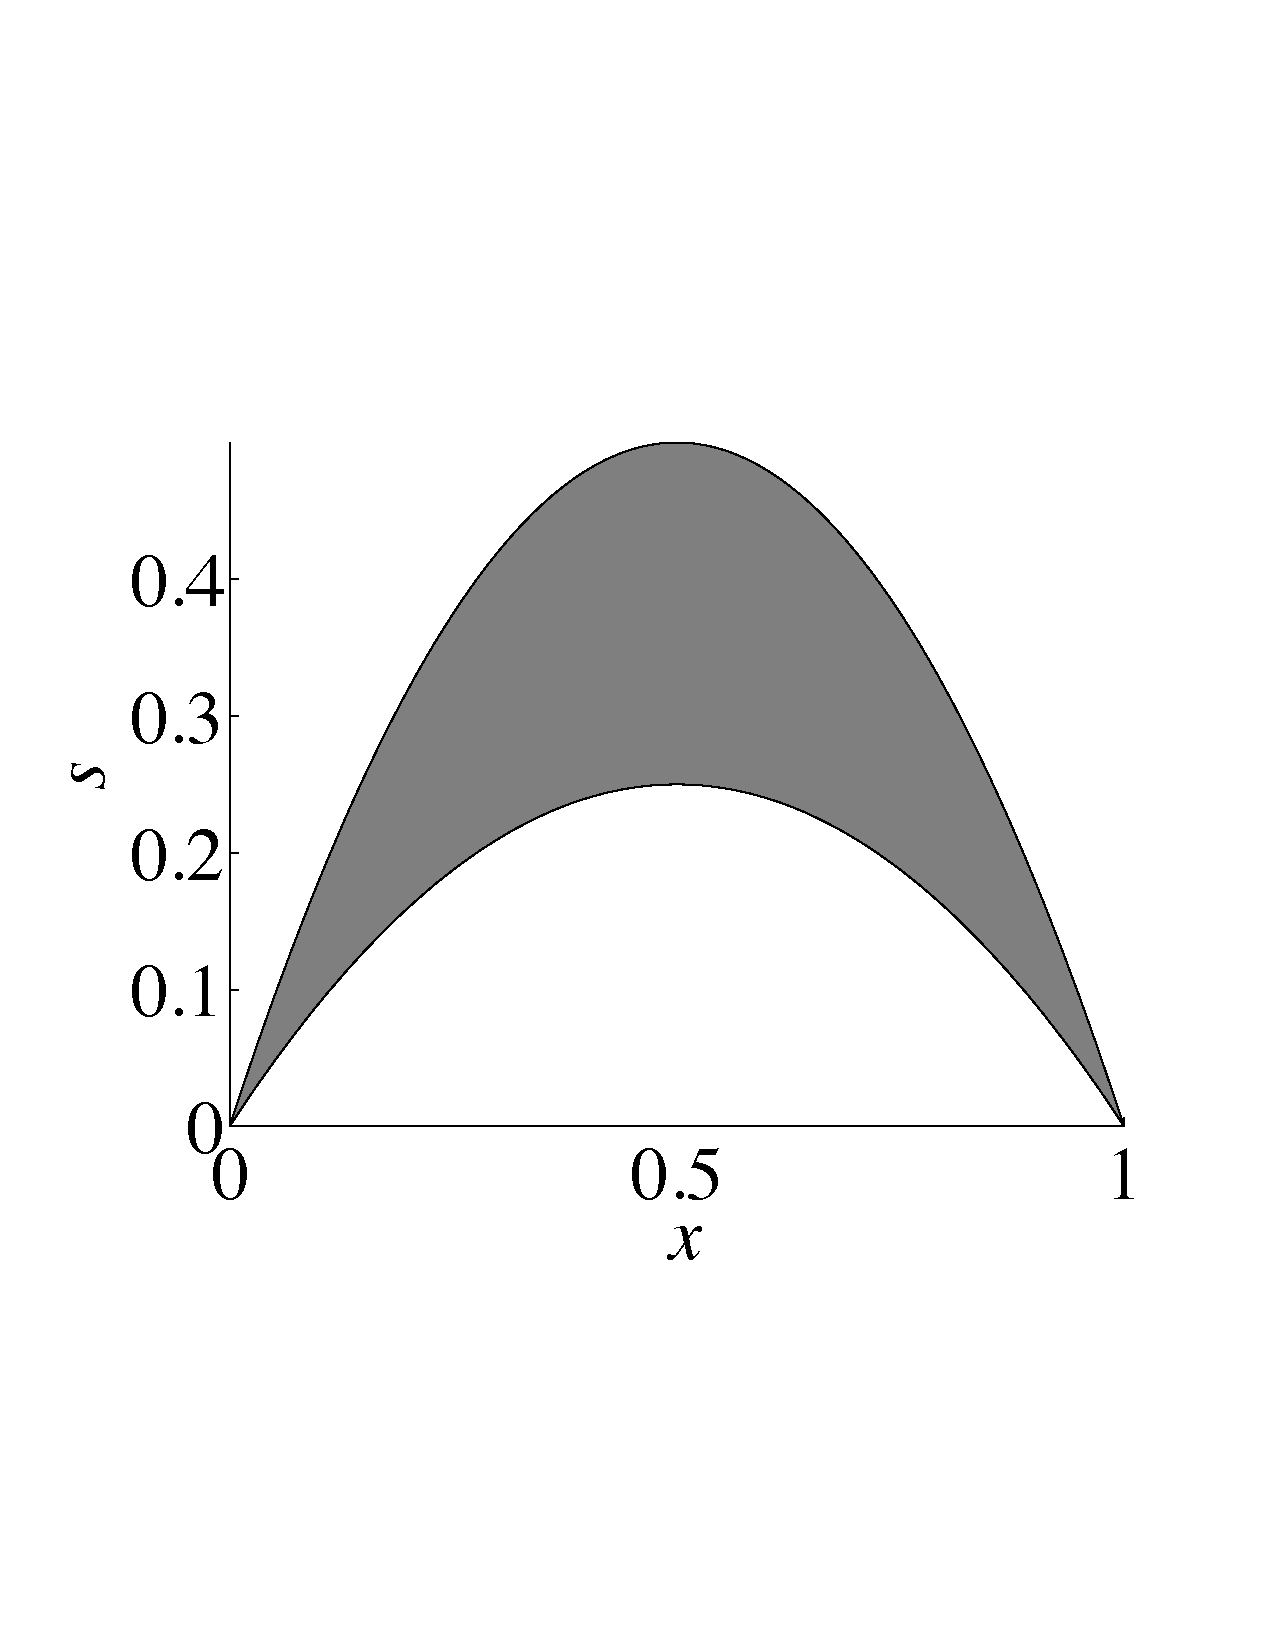
\includegraphics[width=3.5cm]{Figuras/RegionSoporteJun2013.pdf}
\part $\sMSE = \frac{14}{9}x(1-x)$.
\part $\sMAD = \sqrt{\frac{5}{2}}x(1-x)$
\end{parts}
\end{solution}

\fi
%
%%%%%%%%%%%%%%%%%%%%%%%%%%%%%%%%%%%%%%%%%%%%%%%%%%%%%%%%%%%%%%%%
%%%%%%%%%%%%%% Pregunta IV: 
\qformat{\textbf{\ej \thequestion ~~ (ML)} ~~ \linefill}
\ifspanish

\question[25] % MLG

Se toma una medida de la tensión intantánea $x$ existente en un momento dado en un nodo de un circuito. En dicho nodo existe una componente de señal con valor $s$, contaminada por ruido gaussiano aditivo de media nula y varianza $v$, e independiente de la señal. A priori, el valor de $s$ sigue una densidad de probabilidad gaussiana de media y varianza unitarias.

\begin{parts}
\part Suponiendo conocida $v$, calcule el estimador de máxima verosimilitud de $s$, $\hat s_\text{ML}(x)$.
\part Calcule el error cuadrático medio en el que incurre el estimador $\hat s_\text{ML}(x)$.  
\part Calcule la verosimilitud de $v$ a la vista de $x$, $p_{X|v}(x|v)$.
\part Calcule el estimador de máxima verosimilitud de $v$, $\hat v_\text{ML}(x)$.
\end{parts}

\begin{solution}
\begin{parts}
\part $\hat s_\text{ML}(x)=x$
\part $\mathbb{E}[(x-s)^2] = v$
\part $p(x|v) = G(x|1,v+1)$
\part $\hat v_\text{ML}(x) =  \text{máx}[(x-2)x,0]$
\end{parts}
\end{solution}

\else

\question Let $x$ be a measurement of the instantaneous voltage at a circuit node. In such node exists a signal component with value $s$, contaminated by Gaussian aditive noise with mean zero and variance $v$. A priori, the value of $s$
follows a Gaussian pdf with both the mean and variance equal to 1.

\begin{parts}
\part Assuming $v$ is known, obtain the maximum likelihood estimator of $s$, $\hat s_\text{ML}(x)$.
\part Calculate mean square error incurred by estimator $\hat s_\text{ML}(x)$.  
\part Obtain the likelihood of $v$ given $x$, i.e. $p_{X|v}(x|v)$.
\part Calculate the maximum likelihood estimator of $v$, $\hat v_\text{ML}(x)$.
\end{parts}

\begin{solution}
\begin{parts}
\part $\hat s_\text{ML}(x)=x$
\part $\mathbb{E}[(x-s)^2] = v$
\part $p(x|v) = G(x|1,v+1)$
\part $\hat v_\text{ML}(x) =  \text{máx}[(x-2)x,0]$
\end{parts}
\end{solution}

\fi
%
%%%%%%%%%%%%%%%%%%%%%%%%%%%%%%%%%%%%%%%%%%%%%%%%%%%%%%%%%%%%%%%%
%%%%%%%%%%%%% Enero 2014 Q2: Estimación lineal MSE
\qformat{\textbf{\ej \thequestion ~~ (LMSE)} ~~ \linefill}
\ifspanish

\question[20] 

Se sabe que la distribución conjunta de $S$ y $X$ viene dada por:
$$p_{S,X}(s,x) = \frac{4}{(x+s)^3}, \qquad s\ge 1, \quad x\ge 1.  $$

\begin{parts}
\part Determine $p_{S|X}(s|x)$.
\part Determine el estimador MAP de $S$ dado $X$.
\part Determine el estimador de mínima desviación absoluta (MAD) de $S$ dado $X$.
%\part Determine el estimador de mínimo error cuadrático medio (MMSE)
\end{parts}

\begin{solution}
\begin{parts}
\part $p_{S|X}(s|x) = \dfrac{2(x+1)^2}{(x+s)^3}, \qquad, x\ge 1$.
\part $\widehat S_{\text{MAP}}  = 1$.
\part $\widehat S_{\text{MAD}}  = (\sqrt{2}-1) X + \sqrt{2}$.
\end{parts}
\end{solution}

\else

\question[20] 

The joint distribution of $S$ and $X$ is given by:
$$p_{S,X}(s,x) = \frac{4}{(x+s)^3}, \qquad s\ge 1, \quad x\ge 1.  $$

\begin{parts}
\part Find $p_{S|X}(s|x)$.
\part Find the MAP estimator of $S$ given $X$.
\part Find the minimum absolute deviation (MAD) estimator of $S$ given $X$.
%\part Determine el estimador de mínimo error cuadrático medio (MMSE)
\end{parts}

\begin{solution}
\begin{parts}
\part $p_{S|X}(s|x) = \dfrac{2(x+1)^2}{(x+s)^3}, \qquad, x\ge 1$.
\part $\SMAP = 1$.
\part $\SMAD = (\sqrt{2}-1) X + \sqrt{2}$.
\end{parts}
\end{solution}

\fi
%
%%%%%%%%%%%%%%%%%%%%%%%%%%%%%%%%%%%%%%%%%%%%%%%%%%%%%%%%%%%%%%%%
%%%%%%%%%%%%% Enero 2014 P1: Estimación lineal MSE
\qformat{\textbf{\ej \thequestion ~~ (ML)} ~~ \linefill}
\ifspanish

\question[30] % MLG

Un estudiante puntual se levanta temprano cada mañana y alcanza la parada del autobús exactamente a las 8:00 am, que es la hora programada de llegada del único autobus que puede llevarle a la universidad. El bus suele retrasarse y nunca llega antes de su hora prevista. La densidad de probabilidad del retardo del autobús es 
$$
p_{T_\text{B}|\Lambda_\text{B}}(t_\text{B}|\lambda_\text{B}) = \lambda_\text{B} \exp(-\lambda_\text{B} t_\text{B}),~~0<t_\text{B}\text{ min}
$$
donde $t_\text{B}$ son los minutos de retraso. Los retrasos de cada día son independientes e identicamente distribuidos (iid).

Un segundo estudiante, impuntual, utiliza el mismo autobús. El retraso en la llegada de este estudiante a la parada sigue la distribución
$$
p_{T_\text{E}|\Lambda_\text{E}}(t_\text{E}|\lambda_\text{E}) = \lambda_\text{E} \exp(-\lambda_\text{E} t_\text{E}),~~0<t_\text{E}\text{ min}
$$
donde $T_\text{E}$ es el retraso con respecto al estudiante puntual. Estos retrasos también son iid.

Por último, se sabe que $T_\text{B}$ y $T_\text{E}$ son independientes entre sí.

\begin{parts}
\part Modelado: los primeros cinco días del curso el autobús llegó a la parada 0, 6, 15, 20 y 24 minutos tarde, mientras que el estudiante impuntual llegó a la parada 15, 10, 12, 5 y 3 minutos tarde. Estime $\lambda_\text{B}$ y $\lambda_\text{E}$ mediante ML a partir de estas observaciones. Especifique las unidades.

Considere estas estimaciones ML como los verdaderos valores de  $\lambda_\text{B}$ y $\lambda_\text{E}$ durante el resto del ejercicio.

\part Calcule el tiempo medio de espera en la parada del estudiante puntual.
\part El sexto día, el estudiante impuntual llega a la parada a las 8.05 am. Encuentra allí al estudiante puntual y le pregunta cuanto  tiempo más tendrán que esperar (en media) hasta que llegue el autobús. Calcule esta cantidad y contrástela con su respuesta a b).

Indicación: Observe que se está pidiendo calcular ${\mathbb E}[T_\text{B} - 5 \text{ min}|T_\text{B}>5\text{ min}]$.

\part Si el estudiante impuntual pierde el autobús, no irá a la universidad ese día. Suponiendo que este proceso de llegadas del autobús y el estudiante impuntual se repite durante el resto del curso, determine el porcentaje de días que, en media, cada estudiante asiste a la universidad.
\end{parts}

\begin{solution}
\begin{parts}
\part $\hat{\lambda}_\text{B} = \frac{1}{13}\text{ min}^{-1}$, $\hat{\lambda}_\text{V} = \frac{1}{9}\text{ min}^{-1}$.
\part ${\mathbb E}[t_\text{B}]=13\text{ min}$.
\part ${\mathbb E}[t_\text{B} - 5 \text{ min}|t_\text{B}>5\text{ min}] = 13\text{ min}$. Llegar 5 min tarde no le ahorra tiempo de espera, debe esperar (en promedio) lo mismo que espera (en promedio) el alumno puntual los demás días. Esta aparente contradicción se debe a que para el sexto día tenemos un dato adicional: El autobús tendrá un retraso superior a 5 minutos.

\part $P\{t_\text{V}<t_\text{B}\} = \frac{\lambda_\text{v}}{\lambda_\text{v}+\lambda_\text{B}}$, en porcentaje $\frac{100\lambda_\text{v}}{\lambda_\text{v}+\lambda_\text{B}}\%$. El alumno puntual va siempre.
\end{parts}
\end{solution}

\else

\question[30] % MLG

An energetic student gets up early every morning and reaches the bus stop exactly at 8.00 am, the scheduled arrival time of the only bus that  can take take him to the university. The bus is usually late and never arrives before its scheduled arrival time. The pdf of the delay of the bus
$$
p_{T_\text{B}|\Lambda_\text{B}}(t_\text{B}|\lambda_\text{B}) = \lambda_\text{B} \exp(-\lambda_\text{B} t_\text{B}),~~0<t_\text{B}\text{ min}
$$
where $t_\text{B}$ are the minutes of delay. The delays are iid for each day.

A second, lazy student makes use of the same bus, but isn't as punctual as the energetic one. The delay in the arrival of the lazy student to the bus stop follows the  pdf
$$
p_{T_\text{L}|\Lambda_\text{L}}(t_\text{L}|\lambda_\text{L}) = \lambda_\text{L} \exp(-\lambda_\text{L} t_\text{L}),~~0<t_\text{L}\text{ min}
$$
where $T_\text{L}$ is the delay wrt to the energetic student in reaching the bus stop.  These delays are iid for each day.
Finally, $T_\text{B}$ and $T_\text{E}$ are independent.

\begin{parts}
\part Modeling: The first five days of the course the bus arrived to the bus stop 0, 6, 15, 20 and 24 minutes late, whereas the lazy student  arrived to the bus stop  15, 10, 12, 5 and 3 minutes late. Estimate $\lambda_\text{B}$ and $\lambda_\text{L}$ using ML. Specify units.

Consider this ML estimates as the true values for $\lambda_\text{B}$ and $\lambda_\text{L}$ for the remainder of the exercise.

\part Compute the expected waiting time for the energetic student at the bus stop.
\part The sixth day, the lazy student arrives to the bus stop at 8.05 am. He meets there the energetic student and asks him how much longer are both expected  to wait (the expected time) until the bus comes. Compute this quantity and contrast it with your answer to b).

Hint: You are being asked to compute ${\mathbb E}[t_\text{B} - 5 \text{ min}|t_\text{B}>5\text{ min}]$.

\part If the lazy student misses the bus, he won't attend university that day. Assuming this arrival process for the bus and the lazy student is repeated for the rest of the course, compute the \emph{expected} percentage of days that each student attends university.
\end{parts}

\begin{solution}
\begin{parts}
\part $\lambda_\text{B} = \frac{1}{13}\text{ min}^{-1}$, $\lambda_\text{V} = \frac{1}{9}\text{ min}^{-1}$ y ${\mathbb E}[t_\text{B}]=13\text{ min}$.

\part ${\mathbb E}[t_\text{B} - 5 \text{ min}|t_\text{B}>5\text{ min}] = 13\text{ min}$. Arriving 5 min late doesn't save waiting time. On average, he has to wait as much as the willful student the remaining days. This apparent paradox arises from the fact that there is an additional information in the sixth day: the bus will be more than 5 minutes late. 


\part $p(t_\text{V}<t_\text{B}) = \frac{\lambda_\text{v}}{\lambda_\text{v}+\lambda_\text{B}}$, in percentage $\frac{100\lambda_\text{v}}{\lambda_\text{v}+\lambda_\text{B}}\%$. The willful student always goes.
\end{parts}
\end{solution}

\fi
%
%%%%%%%%%%%%%%%%%%%%%%%%%%%%%%%%%%%%%%%%%%%%%%%%%%%%%%%%%%%%%%%%
%%%%%%%%%%%%% Junio 2014 Q2: Estimación lineal MSE
\qformat{\textbf{\ej \thequestion ~~ (MSE)} ~~ \linefill}
\ifspanish

\question[20] % VGV

Las v.a. $S$, $X_1$ y $X_2$ son conjuntamente gaussianas. Se desconocen los parámetros de la distribución conjunta, pero se sabe que:
\begin{itemize}
\item La distribución marginal de $X_1$ y $X_2$ es
$$p_{X_1,X_2}\left ( x_1,x_2\right) \sim G\left (  \left[ \begin{array}{c}   0 \\ 0    \end{array} \right] , \left[ \begin{array}{cc}  1 & \frac{1}{2} \\ \frac{1}{2} & 1  \end{array} \right]\right)$$
\item El estimador de mínimo error cuadrático medio (MMSE) de $S$ empleando solo $X_1$ es:
$$\widehat S_{\text{MMSE},1}=\frac{1}{2} X_1,$$
\item El estimador MMSE de $S$ empleando solo $X_2$ es:
$$\widehat S_{\text{MMSE},2}= X_2.$$
\end{itemize}

Se desea estimar $S$ a la vista de una nueva v.a. $X_3$ dada por la siguiente combinación lineal entre $X_1$ y $X_2$:
$$X_3= X_1 + X_2.$$
%$$X_3=\lambda X_1 + (1-\lambda) X_2,$$
%donde $0\leq \lambda \leq 1$.

\begin{parts}
\part Obtenga el valor medio de $X_3$, $\mathbb E[X_3]$, su varianza, $v_{X_3}$, y su covarianza con $S$, $v_{S,X_3}$.
\part Obtenga el estimador de MMSE de $S$ empleando solo $X_3$, $\widehat S_{\text{MMSE},3}$.
\part Sabiendo que $\mathbb E[S^2]=1$, obtenga el error cuadrático medio del anterior estimador, $\mathbb E[(S-\widehat S_{\text{MMSE},3})^2]$.
\end{parts}

\begin{solution}
\begin{parts}
\part $\mathbb E[X_3]=0$,$v_{X_3}=3$, $v_{S,X_3}=3/2$.
\part $\widehat S_{\text{MMSE},3}= 1/2 X_3$.
\part $\mathbb E[(S-\widehat S_{\text{MMSE},3})^2]=1/4$.

\end{parts}
\end{solution}

\else

\question[20] % VGV

The random variables $S$, $X_1$ and $X_2$ are jointly Gaussian. The parameters of its joint distribution are unknown, but it is known that:
\begin{itemize}
\item The marginal distribution of $X_1$ and $X_2$ is
$$p_{X_1,X_2}\left ( x_1,x_2\right) \sim G\left (  \left[ \begin{array}{c}   0 \\ 0    \end{array} \right] , \left[ \begin{array}{cc}  1 & \frac{1}{2} \\ \frac{1}{2} & 1  \end{array} \right]\right)$$
\item The minimum mean square error (MSE) estimator of $S$ based on $X_1$ only is:
$$\widehat S_{\text{MMSE},1}=\frac{1}{2} X_1,$$
\item The minimum MSE estimator of $S$ based on $X_2$ only is:
$$\widehat S_{\text{MMSE},2}= X_2.$$
\end{itemize}

We want to estimate $S$ given a new random variable $X_3$ given by the following linear combination of $X_1$ and $X_2$
$$X_3= X_1 +  X_2.$$
%$$X_3=\lambda X_1 + (1-\lambda) X_2,$$
%where $0\leq \lambda \leq 1$.

\begin{parts}
\part Compute the mean value of $X_3$, $\mathbb E[X_3]$, its variance, $v_{X_3}$, and its covariance with $S$, $v_{S,X_3}$.
\part Compute the minimum MSE estimator os $S$ based on $X_3$ only, $\widehat S_{\text{MMSE},3}$.
\part Given that $\mathbb E[S^2]=1$, compute the MSE of the estimator computed in the previous section, $\mathbb E[(S-\widehat S_{\text{MMSE},3})^2]$.
\end{parts}

\begin{solution}
\begin{parts}
\part $\mathbb E[X_3]=0$,$v_{X_3}=3$, $v_{S,X_3}=3/2$.
\part $\widehat S_{\text{MMSE},3}= 1/2 X_3$.
\part $\mathbb E[(S-\widehat S_{\text{MMSE},3})^2]=1/4$.

\end{parts}
\end{solution}

\fi
%
%%%%%%%%%%%%%%%%%%%%%%%%%%%%%%%%%%%%%%%%%%%%%%%%%%%%%%%%%%%%%%%%
%%%%%%%%%%%%% Junio 2014 P1
\qformat{\textbf{\ej \thequestion ~~ (Change of variable, LMSE)} ~~ \linefill}
\ifspanish

\question[25] % MLG

Dos variables aleatorias  iid  $X$ y $Y$ siguen una fdp uniforme entre  $0$ y $1$. Se generan dos nuevas variables aleatorias  $U = \max(X,Y)$ y $V = \min(X,Y)$, es decir, se definen $U$ y $V$ como el máximo y el mínimo, respectivamente, de las variables iid uniformes originales.

\begin{parts}
\part Calcule $p_{U|X}(u|x)$ y $p_{V|X}(v|x)$.
\part Calcule $p_{U}(u)$ y $p_{V}(v)$.
\part Calcule $\EE\{U\}$, $\EE\{U^2\}$ y $\EE\{V\}$.
\part Obtenga el estimador lineal de $V$ dado $U$, de mínimo MSE, $\hat{v}_\text{LMSE}(u)$.
\end{parts}

Pista: Dese cuenta de que en apartado (a)  está haciendo un cambio de variable. Puede resultarle útil dibujar $\min(x,y)$ y $\max(x,y)$ como funciones de $y$ para un valor fijo  de $x$. La parte plana que aparece en la gráfica producirá una delta de Dirac en el resultado.

\begin{solution}
\begin{parts}
\part $p_{U|X}(u|x) = x\delta(u-x)+1$ en $x\leq u \leq 1$, y $0$ en otro caso

$p_{V|X}(v|x) = (1-x)\delta(v-x)+1$ en $0\leq v \leq x$, y $0$ en otro caso

\part $p_U(u) = 2u$  en $0\leq u \leq 1$, y $0$ en otro caso

$p_V(v) = 2(1-v)$  en $0\leq v \leq 1$, y $0$ en otro caso

\part $\EE\{U\} = 2/3$, $\EE\{U^2\}=1/2$ and $\EE\{V\}=1/3$
\part $\hat{v}_\text{LMSE}(u)=u/2$.
\end{parts}
\end{solution}

\else

\question[25] % MLG

Two random iid variables $X$ and $Y$ follow a uniform pdf between $0$ and $1$. Two new random variables are generated as $U = \max(X,Y)$ and $V = \min(X,Y)$, i.e., they are defined as the maximum  and minimum, respectively, of the original uniform iid variables.

\begin{parts}
\part Compute $p_{U|X}(u|x)$ and $p_{V|X}(v|x)$.
\part Compute $p_{U}(u)$ and $p_{V}(v)$.
\part Compute $\EE\{U\}$, $\EE\{U^2\}$ and $\EE\{V\}$.
\part Compute the linear estimator of $V$ with minimum MSE given $U$, $\hat{v}_\text{LMSE}(u)$.
\end{parts}

Hint: In case you didn't notice, in part (a)  you are performing a change of variable. You might find it helpful to draw $\min(x,y)$ and $\max(x,y)$ as functions of $y$ for a fixed value of $x$. The flat parts of these two functions will produce Dirac deltas in the corresponding results.

\begin{solution}
\begin{parts}
\part $p_{U|X}(u|x) = x\delta(u-x)+1$ for $x\leq u \leq 1$, and $0$ otherwise

      $p_{V|X}(v|x) = (1-x)\delta(v-x)+1$ for $0\leq v \leq x$, and $0$ otherwise

\part $p_U(u) = 2u$ for $0\leq u \leq 1$, and $0$ otherwise

      $p_V(v) = 2(1-v)$ for $0\leq v \leq 1$, and $0$ otherwise

\part $\EE\{U\} = 2/3$, $\EE\{U^2\}=1/2$ and $\EE\{V\}=1/3$
\part $\hat{v}_\text{LMSE}(u)=u/2$.
\end{parts}
\end{solution}

\fi
%
%%%%%%%%%%%%%%%%%%%%%%%%%%%%%%%%%%%%%%%%%%%%%%%%%%%%%%%%%%%%%%%%
%%%%%%%%%%%%% Enero 2015, Q2 Estimación
\qformat{\textbf{\ej \thequestion ~~ (ML)} ~~ \linefill}
\ifspanish

\question[20] % JCS

Se sabe que la distribución conjunta de $S$ y $X$ viene dada por:
$$p_{X|s}(x|s) = s \exp(-s \exp(-x) + x), \qquad, \quad x \in \mathbb{R}.  $$

\begin{parts}
\part Determine el estimador ML de $S$ dado $x$.
\part Determine el estimador ML de $S$ basado en $K$ observaciones independientes e idénticamente distribuidas, $\{x^{(k)}, k=1,\ldots, K \}$.
\part Suponga que $K=2$ y se observa $x^{(1)}=0$, $x^{(2	)}=-\ln2$. Determine el valor máximo de la verosimilitud para estas observaciones.
\end{parts}

\begin{solution}
\begin{parts}
\part $\hat{S}_{\text{ML}} = \exp(X)$.
\begin{align*}
\hat{s}_{\text{ML}} 
	&= \argmax_s \log p_{X|S}(x|s)  \\
	&= \argmax_s \log \left(s \exp\left(-s \exp(-x) + x\right) \right)  \\
	&= \argmax_s \left( \log s -s \exp(-x) + x \right)  \\
	&= \exp(x)
\end{align*}
\part 
\begin{align*}
\hat{s}_{\text{ML}} 
	&= \argmax_s \sum_{k=1}^K \log p_{X|S}(x^{(k)}|s)  \\
	&= \argmax_s \sum_{k=1}^K \log \left(s \exp\left(-s \exp\left(-x^{(k)}\right) + x^{(k)}\right)\right)  \\
	&= \argmax_s \left( K\log s -s \sum_{k=1}^K\exp\left(-x^{(k)}\right) + \sum_{k=1}^Kx^{(k)}\right)  \\
	&= \dfrac{K}{\sum_{k=1}^K \exp(-x^{(k)})}
\end{align*}
\part $p_{X^{(1)},X^{(2)}|s}(0,-\ln(2)|\hat{s}_{\text{ML}}) = \dfrac{2\exp(-2)}{9}$.
\end{parts}
\end{solution}

\else

\question[20] % JCS

The joint distribution of random variables $S$ and $X$ is known to be:
$$p_{X|s}(x|s) = s \exp(-s \exp(-x) + x), \qquad, \quad x \in \mathbb{R}.  $$

\begin{parts}
\part Compute the ML estimate of $S$ given $x$.
\part Compute the ML estimate of $S$ given $K$ independent and identically distributed observations, $\{X^{(k)}, k=1,\ldots, K \}$.
\part Let $K=2$ and assume that $x^{(1)}=0$, $x^{(2	)}=-\ln2$. Compute the value of the maximum likelihood for these observations.
\end{parts}

\begin{solution}
\begin{parts}
\part $\hat{S}_{\text{ML}} = \exp(X)$.
\begin{align*}
\hat{s}_{\text{ML}} 
	&= \argmax_s \log p_{X|S}(x|s)  \\
	&= \argmax_s \log \left(s \exp\left(-s \exp(-x) + x\right) \right)  \\
	&= \argmax_s \left( \log s -s \exp(-x) + x \right)  \\
	&= \exp(x)
\end{align*}
\part 
\begin{align*}
\hat{s}_{\text{ML}} 
	&= \argmax_s \sum_{k=1}^K \log p_{X|S}(x^{(k)}|s)  \\
	&= \argmax_s \sum_{k=1}^K \log \left(s \exp\left(-s \exp\left(-x^{(k)}\right) + x^{(k)}\right)\right)  \\
	&= \argmax_s \left( K\log s -s \sum_{k=1}^K\exp\left(-x^{(k)}\right) + \sum_{k=1}^Kx^{(k)}\right)  \\
	&= \dfrac{K}{\sum_{k=1}^K \exp(-x^{(k)})}
\end{align*}
\part $p_{X^{(1)},X^{(2)}|s}(0,-\ln(2)|\hat{s}_{\text{ML}}) = \dfrac{2\exp(-2)}{9}$.
\end{parts}
\end{solution}

\fi
%
%%%%%%%%%%%%%%%%%%%%%%%%%%%%%%%%%%%%%%%%%%%%%%%%%%%%%%%%%%%%%%%%
%%%%%%%%%%%%%% Enero 2015, Q4
\qformat{\textbf{\ej \thequestion ~~ (ML, MAP, MSE)} ~~ \linefill}
\ifspanish

\question[25] % VGV

Se desea estimar el valor de la v.a. $S$ a partir de la observación de otra variable aleatoria $X$, que se genera a partir de $S$ mediante la siguiente relación
$$X = S -R $$
siendo $R$ una v.a. independiente de $S$ con distribución
$$p_R(r) = \text{exp}(-r), ~~r>0$$
\begin{parts}
 		\part Obtenga el estimador de máxima verosimilitud de $S$ a la vista de $X$, $\hat S_\text{ML}$.
\end{parts}
Sabiendo que la f.d.p. de $S$ es $p_S(s) = \text{exp}(-s), ~~s>0$, calcule:
\begin{parts}
\setcounter{partno}{1}
 		\part  El estimador de máximo a posteriori de $S$ a la vista de $X$, $\hat S_\text{MAP}$. 
 		\part El estimador de mínimo error cuadrático medio de $S$ a la vista de $X$, $\hat S_\text{MMSE}$. 
\end{parts}

\begin{solution}
\begin{parts}
 		\part  $p_{X|S}(x|s) = \text{exp}(x-s), ~~x<s$. \\
 		$\hat S_\text{ML} = X$. 
 		\part  $p_{X,S}(x,s) = \text{exp}\left( -x-2s \right), ~~s >0; ~x<s$;\\
 		 $\hat S_\text{MAP} =
 			\left\lbrace \begin{array}{ll}
        	 		0 &\quad {\rm si }~~ x<0\\
        	 		x & \quad {\rm si } ~~x>0
        		\end{array}  \right. $ 		 
        \part $p_{S|X} = \left\lbrace \begin{array}{ll}
        	 2\text{exp}\left( -2s\right), ~~ s >0 &\quad {\rm si }~~ x<0\\
        	 2\text{exp}\left( 2x\right)\text{exp}\left( -2s\right), ~~ s >x & \quad {\rm si } ~~x>0
        \end{array}         \right. $ \\
          $\hat S_\text{MMSE} =  \left\lbrace \begin{array}{ll}
        	 \frac{1}{2} &\quad {\rm si }~~ x<0\\
        	 \frac{1}{2}+x & \quad {\rm si } ~~x>0
        \end{array}         \right. $
        
\end{parts}
\end{solution}

\else

\question[25] % VGV

We want to estimate the value of a random variable $S$ using a random observation $X$, which is related to $S$ via
$$X = S-R $$
where $R$ is a r.v. independent of $S$ with p.d.f.
$$p_R(r) = \text{exp}(-r), ~~r>0$$
\begin{parts}
 		\part Find the maximum likelihood estimator of $S$ given $X$, $\hat S_\text{ML}$.
\end{parts}
Knowing also that the p.d.f. of $S$ is $p_S(s) = \text{exp}(-s), ~~s>0$, obtain:
\begin{parts}
\setcounter{partno}{2}
 	\part  The maximum {\em a posteriori} estimator of $S$ given $X$, $\hat S_\text{MAP}$.
 	\part The minimum mean square error estimator of $S$ given $X$, $\hat S_\text{MMSE}$. 
\end{parts}

\begin{solution}
\begin{parts}
 		\part  $p_{X|S}(x|s) = \text{exp}(x-s), ~~x<s$. \\
 		$\hat S_\text{ML} = X$. 
 		\part  $p_{X,S}(x,s) = \text{exp}\left( -x-2s \right), ~~s >0; ~x<s$;\\
 		 $\hat S_\text{MAP} =
 			\left\lbrace \begin{array}{ll}
        	 		0 &\quad {\rm if }~~ x<0\\
        	 		x & \quad {\rm if } ~~x>0
        		\end{array}  \right. $ 		 
        \part $p_{S|X} = \left\lbrace \begin{array}{ll}
        	 2\text{exp}\left( -2s\right), ~~ s >0 &\quad {\rm si }~~ x<0\\
        	 2\text{exp}\left( 2x\right)\text{exp}\left( -2s\right), ~~ s >x & \quad {\rm if } ~~x>0
        \end{array}         \right. $ \\
          $\hat S_\text{MMSE} =  \left\lbrace \begin{array}{ll}
        	 \frac{1}{2} &\quad {\rm if }~~ x<0\\
        	 \frac{1}{2}+x & \quad {\rm if } ~~x>0
        \end{array}         \right. $
        
\end{parts}
\end{solution}

\fi
%
%%%%%%%%%%%%%%%%%%%%%%%%%%%%%%%%%%%%%%%%%%%%%%%%%%%%%%%%%%%%%%%%
%%%%%%%%%%%%% Junio 2015, Q2
\qformat{\textbf{\ej \thequestion ~~ (ML)} ~~ \linefill}
\ifspanish

\question[20] % JCS

La variable aleatoria $X$ está dada por la función de verosimilitud
\[
p_{X|S}(x|s) = \ln\left(\dfrac{1}{s}\right) s^x , \qquad x\ge 0, \qquad  0\le s \le 1
\]
siendo $s$ un parámetro desconocido.
\begin{parts}
\part Determine el estimador ML de $s$ a la vista de $x$.
\part Determine la verosimilitud máxima para $x=1$.
\part Determine el estimador ML de $s$ a la vista de un conjunto $\mathcal{C} = \{x_k, k=0,\ldots,K-1\}$ de $K$ realizaciones independientes de $X$. 
\end{parts}

\begin{solution}
\begin{parts}
\part $\SML = \exp\left(-\dfrac{1}{X}\right)$ 
\part $p_{X|S}(1|s_{\text{ML}}) = \dfrac{1}{e}$
\part $\SML = \exp\left(-\dfrac{K}{\sum_{k=0}^{K-1} x_k} \right)$ 
\end{parts}
\end{solution}

\else

\question[20] % JCS

Random variable $X$ is driven by the likelihood function
\[
p_{X|S}(x|s) = \ln\left(\dfrac{1}{s}\right) s^x , \qquad x\ge 0, \qquad  0\le s \le 1
\]
where $s$ is an unknown parameter.

\begin{parts}
\part Compute the ML estimate of $s$ given $x$.
\part Compute the value of the maximum likelihood for $x=1$.
\part Compute the ML estimate of $s$ given $K$ a set $\mathcal{C} = \{x_k, k=0,\ldots,K-1\}$ of $K$ independent realizations of $X$. 
\end{parts}

\begin{solution}
\begin{parts}
\part $\SML = \exp\left(-\dfrac{1}{X}\right)$ 
\part $p_{X|S}(1|s_{\text{ML}}) = \dfrac{1}{e}$
\part $\SML = \exp\left(-\dfrac{K}{\sum_{k=0}^{K-1} x_k} \right)$ 
\end{parts}
\end{solution}

\fi
%
%%%%%%%%%%%%%%%%%%%%%%%%%%%%%%%%%%%%%%%%%%%%%%%%%%%%%%%%%%%%%%%%
%%%%%%%%%%%%%% Junio 2015, Q4
\qformat{\textbf{\ej \thequestion ~~ (ML, MAP, MSE)} ~~ \linefill}
\ifspanish

\question[25] % VGV

Se desea estimar el valor de la v.a. $S$ a partir de la observación de otra variable aleatoria $X$, de las que se conoce su distribución conjunta
$$p_{S,X}(s,x) = 4x,  \qquad 0 \le s \le x^2, ~~ 0 \le x \le 1$$
Obtenga:
\begin{parts}
\part El estimador de máxima verosimilitud de $S$ a la vista de $X$, $\SML$.
\part El estimador de máximo a posteriori de $S$ a la vista de $X$, $\SMAP$. 
\part El estimador de mínimo error cuadrático medio de $S$ a la vista de $X$, $\SMSE$.
\part El estimador lineal de  mínimo error cuadrático medio de $S$ a la vista de $X$, $\SLMSE = w_0+w_1x$.
\end{parts}

\begin{solution}
\begin{parts}
\part 
The prior distribution is
\begin{align*}
p_S(s) &= \int_{-\infty}^{\infty} p_{S,X}(s,x) dx
	    = \int_{\sqrt{s}}^{1} 4x dx = 2(1 - s)   
\end{align*}
Therefore, the likelihood function is
\begin{align*}
p_{X|S}(x|s) &= \frac{p_{X,S}(x,s)}{p_S(s)} 
	          = \frac{x}{1-s}            \qquad 0 \le s \le x^2, \qquad 0 \le x \le 1
\end{align*}
which is an increasing function of $s$. Thus, the ML estimate is the maximum value of $s$ in the domain of the likelihood function, that is
$$\SML = X^2$$

\part 
\begin{align*}
\sMAP = \argmax_s p_{S|X}(s|x) 
	  = \argmax_s p_{S,X}(s, x) 
	  = \argmax_s 4x 
\end{align*}
Thus, $\SMAP$ is not unique: any value of $s \in [0,X^2]$ is a MAP estimate.
\part
Since the marginal distribution is
\begin{align*}
p_X(x) &= \int_{-\infty}^{\infty} p_{S,X}(s,x) ds
	    = \int_0^{x^2} 4x ds = 4x^3
\end{align*}
the posterior distribution is
\begin{align*}
p_{S|X}(s|x) &= \frac{p_{X,S}(x,s)}{p_X(x)} 
	          = \frac{1}{x^2}            \qquad 0 \le s \le x^2 \le 1
\end{align*}
Therefore
\begin{align*}
\sMSE
	&= \EE\{S|x\} 
	 = \int_{-\infty}^{\infty} s p_{S|X}(s|x) ds
	 = \int_0^{x^2} \frac{s}{x^2} ds = \frac{x^2}{2} 	 
\end{align*}
\part Since $\SLMSE = {\bf w}^\intercal {\bf Z}$, where ${\bf Z} = (1, X)^\intercal$, we have
\begin{align*}
{\bf w} 
    &= {\bf R}_{\bf Z}^{-1}{\bf r}_{S{\bf Z}}  \\
{\bf R}_{\bf Z}
    &= \EE\{{\bf Z}{\bf Z}^\intercal\} 
     = \begin{pmatrix} 
       1        & \EE\{X\}   \\
       \EE\{X\} & \EE\{X^2\} 
       \end{pmatrix}  \\
{\bf r}_{S{\bf Z}}
    &= \EE\{S{\bf Z}\} 
     = \begin{pmatrix} \EE\{S\} \\ \EE\{SX\} \end{pmatrix}
\end{align*}
Noting that
\begin{align*}
\EE\{X\}   &= \int_0^1 4x^4 dx = \frac45   \\
\EE\{X^2\} &= \int_0^1 4x^5 dx = \frac23   \\
\EE\{S\}   &= \int_0^1 2s(1-s) ds = \frac13   \\
\EE\{SX\}
	&= \int_0^1 \EE\{Sx|x\}p_X(x) dx 
     = \int_0^1 \frac{x^3}{2} 4x^3 dx = \frac27
\end{align*}
we get
\begin{align*}
{\bf w} 
    &= \begin{pmatrix} 
       1       & \frac45  \\
       \frac45 & \frac23 
       \end{pmatrix}^{-1} 
       \begin{pmatrix} 
       \frac13   \\  \frac27 
       \end{pmatrix}
     = \begin{pmatrix} 
       -\frac5{21} \\ \frac57 
       \end{pmatrix}
\end{align*}
Thus
$\SLMSE =  \frac57 X - \frac5{21} $
\end{parts}
\end{solution}

\else

\question[25] % VGV

We want to estimate the value of a random variable $S$ using a random observation $X$, from which the joint probability distribution is known
$$p_{S,X}(s,x) = 4x,  \qquad 0 \le s \le x^2, \qquad 0 \le x \le 1$$
Obtain:
\begin{parts}
\part The maximum likelihood estimator of $S$ given $X$, $\SML$.
\part The maximum {\em a posteriori} estimator of $S$ given $X$, $\SMAP$.
\part The minimum mean square error estimator of $S$ given $X$, $\SMSE$. 
\part The linear estimator of $S$, with minimum mean square error, given $X$, $\SLMSE=w_0+w_1x$.
\end{parts}

\begin{solution}
\begin{parts}
\part 
The prior distribution is
\begin{align*}
p_S(s) &= \int_{-\infty}^{\infty} p_{S,X}(s,x) dx
	    = \int_{\sqrt{s}}^{1} 4x dx = 2(1 - s)   
\end{align*}
Therefore, the likelihood function is
\begin{align*}
p_{X|S}(x|s) &= \frac{p_{X,S}(x,s)}{p_{S}(s)} 
	          = \frac{x}{1-s}            \qquad 0 \le s \le x^2, \qquad 0 \le x \le 1
\end{align*}
which is an increasing function of $s$. Thus, the ML estimate is the maximum value of $s$ in the domain of the likelihood function, that is
$$\SML = X^2$$

\part 
\begin{align*}
\sMAP = \argmax_s p_{S|X}(s|x) 
	  = \argmax_s p_{S,X}(s, x) 
	  = \argmax_s 4x 
\end{align*}
Thus, $\SMAP$ is not unique: any value of $s \in [0,X^2]$ is a MAP estimate.
\part
Since the marginal distribution is
\begin{align*}
p_X(x) &= \int_{-\infty}^{\infty} p_{S,X}(s,x) ds
	    = \int_0^{x^2} 4x ds = 4x^3
\end{align*}
the posterior distribution is
\begin{align*}
p_{S|X}(s|x) &= \frac{p_{X,S}(x,s)}{p_X(x)} 
	          = \frac{1}{x^2}            \qquad 0 \le s \le x^2 \le 1
\end{align*}
Therefore
\begin{align*}
\sMSE
	&= \EE\{S|x\} 
	 = \int_{-\infty}^{\infty} s p_{S|X}(s|x) ds
	 = \int_0^{x^2} \frac{s}{x^2} ds = \frac{x^2}{2} 	 
\end{align*}
\part Since $\SLMSE = {\bf w}^\intercal {\bf Z}$, where ${\bf Z} = (1, X)^\intercal$, we have
\begin{align*}
{\bf w} 
    &= {\bf R}_{\bf Z}^{-1}{\bf r}_{S{\bf Z}}  \\
{\bf R}_{\bf Z}
    &= \EE\{{\bf Z}{\bf Z}^\intercal\} 
     = \begin{pmatrix} 
       1        & \EE\{X\}   \\
       \EE\{X\} & \EE\{X^2\} 
       \end{pmatrix}  \\
{\bf r}_{S{\bf Z}}
    &= \EE\{S{\bf Z}\} 
     = \begin{pmatrix} \EE\{S\} \\ \EE\{SX\} \end{pmatrix}
\end{align*}
Noting that
\begin{align*}
\EE\{X\}   &= \int_0^1 4x^4 dx = \frac45   \\
\EE\{X^2\} &= \int_0^1 4x^5 dx = \frac23   \\
\EE\{S\}   &= \int_0^1 2s(1-s) ds = \frac13   \\
\EE\{SX\}
	&= \int_0^1 \EE\{Sx|x\}p_X(x) dx 
     = \int_0^1 \frac{x^3}{2} 4x^3 dx = \frac27
\end{align*}
we get
\begin{align*}
{\bf w} 
    &= \begin{pmatrix} 
       1       & \frac45  \\
       \frac45 & \frac23 
       \end{pmatrix}^{-1} 
       \begin{pmatrix} 
       \frac13   \\  \frac27 
       \end{pmatrix}
     = \begin{pmatrix} 
       -\frac5{21} \\ \frac57 
       \end{pmatrix}
\end{align*}
Thus
$\SLMSE =  \frac57 X - \frac5{21} $
\end{parts}
\end{solution}

\fi
%
%%%%%%%%%%%%%%%%%%%%%%%%%%%%%%%%%%%%%%%%%%%%%%%%%%%%%%%%%%%%%%%%
%%%%%%%%%%%%% Enero 2016, Q2
\qformat{\textbf{\ej \thequestion ~~ (ML)} ~~ \linefill}
\ifspanish

\question[20] % JCS

La variable aleatoria $X$ sigue la siguiente función de densidad de probabilidad:
\[
p_{X}(x) = a^2 x \exp\left(-a x \right) , \qquad x\ge 0
\]
siendo $a$ un parámetro desconocido.
\begin{parts}
\part Determine la expresión del estimador ML de $a$ a la vista de un conjunto $\mathcal{C} = \{ x_k, k=0,\ldots ,K-1\}$ de $K$ realizaciones independientes de $X$.
\part Dado el conjunto de observaciones $\mathcal{C} = \{0.2, 0.5, 0.8, 1\}$, determine el valor de $\hat A_{\text{ML}}$.% y obtenga el valor de la verosimilitud de $A_{\text{ML}}$ sobre dicho conjunto de observaciones.
\end{parts}

\begin{solution}
\begin{parts}
\part $\hat A_{\text{ML}} = \dfrac{2K}{\sum_{k=0}^{K-1} x_k}$ 
\part $\hat A_{\text{ML}} = 3.2 $%, $p_{\bf X}({\bf x}|a_{\text{ML}}) = 0.295$
\end{parts}
\end{solution}



\else

\question[20] % JCS

Random variable $X$ is characterized by the following density:
\[
p_X(x) = a^2 x \exp\left(-a x \right) , \qquad x\ge 0
\]
where $a$ is an unknown parameter.
\begin{parts}
\part Obtain the expression of the ML estimator of $a$ for a given set $\mathcal{C} = \{x_k, k=0,\ldots, K-1\}$ of $K$ independent realizations of $X$.

\part Given the set of observations $\mathcal{C} = \{0.2, 0.5, 0.8, 1\}$, find the value of $\hat A_{\text{ML}}$. % and calculate the likelihood of $A_{\text{ML}}$ for such set of observations.
\end{parts}

\begin{solution}
\begin{parts}
\part $\hat A_{\text{ML}} = \dfrac{2K}{\sum_{k=0}^{K-1} x_k}$ 
\part $\hat A_{\text{ML}} = 3.2 $%, $p_{\bf X}({\bf x}|a_{\text{ML}}) = 0.295$
\end{parts}
\end{solution}


\fi
%
%%%%%%%%%%%%%%%%%%%%%%%%%%%%%%%%%%%%%%%%%%%%%%%%%%%%%%%%%%%%%%%%
%%%%%%%%%%%%%% Enero 2016, Q4
\qformat{\textbf{\ej \thequestion ~~ (LMSE)} ~~ \linefill}
\ifspanish

\question[25]  %JAG

%Una compañía energética dispone de tres parques de generación eólica. La potencia total generada a partir de este tipo de energía puede modelarse como
%$$S = 10 (2 X_1 + X_2 + X_3),$$
%donde $S$ es la potencia generada, y $X_i,~i=1, 2, 3,$ es la velocidad del viento en cada instalación. Se sabe que la distribución conjunta de $X_1$ y $X_2$ es
%\begin{equation}
%p_{X_1,X_2}(x_1,x_2) = \frac{1}{a~b} \exp\left(-\frac{x_1}{a}\right), ~~~\text{para } 0<x_1<\infty ~~~\text{y } x_1 < x_2 < x_1 + b
%\end{equation}
%con $a = 30$ y $b = a \ln 2$. Además, se sabe que $\mathbb{E}\{X_3\} = 30$ y que dicha variable $X_3$ es independiente de $X_1$ y $X_2$.
%
%Se desea construir un estimador lineal de mínimo error cuadrático de $S$ basado en las observaciones ${X_1}$ y $X_2$. Para ello:
%
%\begin{parts}
%\part Represente el dominio de la distribución conjunta de $X_1$ y $X_2$.
%\part Calcule la correlación de $X_1$ y $X_2$: $\mathbb{E}\{X_1 X_2\}$.
%\part Obtenga la distribución marginal de $X_1$, y la media y varianza de dicha variable.
%\part Obtenga la distribución marginal de $X_2$. Observe en su resolución que la expresión analítica de dicha distribución difiere para $X_2 < b$ y $X_2 > b$. Calcule la media y varianza de $X_2$.
%\part Obtenga los pesos óptimos del estimador LMSE de $S$:
%$\hat{S}_\text{LMSE} = w_0^\ast + w_1^\ast X_1 + w_2^\ast X_2$ 
%\end{parts}
%
%Indicación: $$\begin{pmatrix} a & b \\c & d \end{pmatrix}^{-1}=\frac{1}{ad-bc}\begin{pmatrix} \phantom{-}d & -b \\-c & \phantom{-}a \end{pmatrix}$$

Una compañía energética dispone de dos parques de generación eólica. La potencia total generada a partir de estos recursos puede modelarse como
$$S = 10 (2 X_1 + X_2),$$
donde $S$ es la potencia generada, y $X_i,~i=1, 2,$ es la velocidad del viento en cada instalación. Se sabe que la distribución conjunta de $X_1$ y $X_2$ es
\begin{equation}
	p_{X_1,X_2}(x_1,x_2) = \frac{1}{a~b} \exp\left(-\frac{x_1}{a}\right), ~~~\text{para } 0<x_1<\infty ~~~\text{y }~~~x_1 < x_2 < x_1 + b
\end{equation}
con $b = a \ln 2$. 

Se desea construir un estimador lineal de mínimo error cuadrático de $S$ basado en la observación ${X_1}$. Para ello:

\begin{parts}
	\part Represente el dominio de la distribución conjunta de $X_1$ y $X_2$.
	\part Obtenga la distribución marginal de $X_1$. Calcule la media y el valor cuadrático medio de dicha variable.
	\part Calcule la media de $X_2$ y la correlación de $X_1$ y $X_2$: $\mathbb{E}\{X_1 X_2\}$.
%	\part Obtenga la distribución marginal de $X_2$. Observe en su resolución que la expresión analítica de dicha distribución difiere para $X_2 < b$ y $X_2 > b$. Calcule la media de $X_2$.
	\part Obtenga los pesos óptimos del estimador LMSE de $S$ buscado:
	$\hat{S}_\text{LMSE} = w_0^\ast + w_1^\ast X_1$ 
\end{parts}

\begin{solution}
\begin{parts}
\setcounter{partno}{1}
\part $p_{X_1}(x_1) = \frac{1}{a} \exp\left(-\frac{x_1}{a}\right),$ for $x_1 > 0$

$\mathbb{E}\{X_1\} = a$ y $\mathbb{E}\{X_1^2\} = 2 a^2$
\part $\mathbb{E}\{X_2\} = a + \frac{b}{2}$

$\mathbb{E}\{X_1 X_2\} = 2a^2 + \frac{b a }{2}$

\end{parts}
\end{solution}


\else
%
\question[25] 

An electric company owns two wind farms. The total generated power can be modeled as
$$S = 10 (2 X_1 + X_2),$$
where $S$ is the generated power, and $X_i,~i=1, 2,$ represents wind speed at each farm. It is further known that the joint distribution of $X_1$ and $X_2$ is given by
\begin{equation}
p_{X_1,X_2}(x_1,x_2) = \frac{1}{a~b} \exp\left(-\frac{x_1}{a}\right), ~~~\text{for } 0<x_1<\infty ~~~\text{and }~~~x_1 < x_2 < x_1 + b
\end{equation}
with $b = a \ln 2$. 

We wish to design a linear minimum mean square error estimator of $S$ based just on observation $X_1$. In order to do so:

\begin{parts}
	\part Sketch the support of the joint distribution of  $X_1$ and $X_2$.
	\part Obtain the marginal distribution of $X_1$. Calculate the mean and mean square value of such variable.
	\part Find the mean of $X_2$ and the correlation between  $X_1$ and $X_2$: $\mathbb{E}\{X_1 X_2\}$.
	% \part Obtenga la distribución marginal de $X_2$. Observe en su resolución que la expresión analítica de dicha distribución difiere para $X_2 < b$ y $X_2 > b$. Calcule la media de $X_2$.
	\part Find the optimum weights of the desired LMSE estimator. 
	$\hat{S}_\text{LMSE} = w_0^\ast + w_1^\ast X_1$ 
\end{parts}

\begin{solution}
	\begin{parts}
		\setcounter{partno}{1}
		\part $p_{X_1}(x_1) = \frac{1}{a} \exp\left(-\frac{x_1}{a}\right),$ for $x_1 > 0$
		
		$\mathbb{E}\{X_1\} = a$ y $\mathbb{E}\{X_1^2\} = 2 a^2$
		\part $\mathbb{E}\{X_2\} = a + \frac{b}{2}$
		
		$\mathbb{E}\{X_1 X_2\} = 2a^2 + \frac{b a }{2}$
		
	\end{parts}
\end{solution}

\fi
%
%%%%%%%%%%%%%%%%%%%%%%%%%%%%%%%%%%%%%%%%%%%%%%%%%%%%%%%%%%%%%%%%
%%%%%%%%%%%%% Junio 2016, Q2
\qformat{\textbf{\ej \thequestion ~~ (MSE)} ~~ \linefill}
\ifspanish

\question[20] % JCS

La distribución conjunta de dos variables aleatorias $S$ y $X$ está dada por:
\[
p_{S,X}(s,x) = \sqrt{\frac{x(1-x)}{2\pi}} \exp\left(-\frac{(s-x(1-x))^2}{2x(1-x)} \right) , \qquad 0 < x < 1, \qquad s \in \mathbb{R}  
\]
\begin{parts}
\part Determine el estimador de mínimo error cuadrático medio de $S$ a la vista de $x$.
\part Determine el error cuadrático medio condicionado a la observación, $\mathbb{E}\{(S-\widehat{S}_{\text{MMSE}})^2|X=x\}$ para el estimador obtenido en el apartado a).
\part Determine el error cuadrático medio del estimador obtenido en el apartado a).
\end{parts}

\begin{solution}
\begin{parts}
\part $\widehat{S}_{\text{MMSE}} = X (1-X)$ 
\part $\mathbb{E}\{(S-\widehat{S}_{\text{MMSE}})^2|X=x\} = x (1-x)$
\part $\mathbb{E}\{(S-\widehat{S}_{\text{MMSE}})^2\} = \dfrac{1}{30}$
\end{parts}
\end{solution}


\else

\question[20] % JCS

The joint distribution of random variables $S$ and $X$ is given by:
\[
p_{S,X}(s,x) = \sqrt{\frac{x(1-x)}{2\pi}} \exp\left(-\frac{(s-x(1-x))^2}{2x(1-x)} \right) , \qquad 0 < x < 1, \qquad s \in \mathbb{R} 
\]
\begin{parts}
\part Determine the minimum mean square error estimate of $S$ based on the observation $x$.
\part Determine the conditional mean square error given observation $x$, $\mathbb{E}\{(S-\widehat{S}_{\text{MMSE}})^2|X=x\}$, for the estimator obtained in part a).
\part Determine the mean square error of the estimator obtained in part a).
\end{parts}

\begin{solution}
\begin{parts}
\part $\widehat{S}_{\text{MMSE}} = X (1-X)$ 
\part $\mathbb{E}\{(S-\widehat{S}_{\text{MMSE}})^2|X=x\} = x (1-x)$
\part $\mathbb{E}\{(S-\widehat{S}_{\text{MMSE}})^2\} = \dfrac{1}{30}$
\end{parts}
\end{solution}

\fi
%
%%%%%%%%%%%%%%%%%%%%%%%%%%%%%%%%%%%%%%%%%%%%%%%%%%%%%%%%%%%%%%%%
%%%%%%%%%%%%%% Junio 2016, Q4
\qformat{\textbf{\ej \thequestion ~~ (MSE)} ~~ \linefill}
% !TeX spellcheck = en_US
\ifspanish

\question[25]  %VGV

%Se sabe que en un sistema de comunicación estándar al receptor le llega una observación $X$ generada a partir de la suma de la señal transmitida más un ruido independiente. Para mejorar las prestaciones de este sistema, 
Una empresa de investigación está trabajando en nuevo sistema de comunicaciones que le permite modelar la distribución de ruido antes de mezclarse con la señal. De este modo, al receptor le llega la siguiente observación
$$ X= S+N_{\rm mod}$$

donde la señal $S$ es una v.a. gaussiana de media nula y varianza $v_s$, y $N_{mod}$ es el nuevo ruido que viene dado por la siguiente expresión:
$$N_{\rm mod} = \lambda  N_1 + (1-\lambda) N_2$$

siendo $N_1$, $N_2$  v.a. gaussianas independientes entre sí, e independientes de $S$, con media nula y varianza $v$; mientras que  $\lambda$ es un parámetro de control del sistema que puede tomar valores en el rango de $0$ a $1$.

\begin{parts}
\part Obtenga la distribución de $N_{\rm mod}$ en función de $\lambda$.
\part Calcule el estimador de mínimo MSE de $S$ a la vista de $X$ para el nuevo sistema y obtenga el error cuadrático medio de dicho modelo en función de $\lambda$.
\part Calcule el valor de $\lambda$, $\lambda_{\rm opt}$, que proporcionaría el menor error cuadrático posible. 
\part Indique, en términos de reducción del MSE, la ventaja que proporcionaría este modelo cuando se configura con el valor $\lambda_{\rm opt}$ respecto al caso $\lambda =0$ o $\lambda =1$. Obtenga esta reducción del error para el caso particular en el que $v_s= v = 1$.
\end{parts}

El técnico encargado de diseñar el sistema que genera $N_{\rm mod}$ se ha ido de vacaciones, dejando el sistema funcionando pero sin indicar con qué valor de $\lambda$ lo ha dejado configurado. Así que le piden al nuevo estudiante en prácticas que tome un conjunto de observaciones independientes del ruido a la salida del prototipo, $\{N_{\rm mod}^{(k)}\}_{k=0}^{K-1}$, y estime por máxima verosimilitud el valor de $\lambda$, $\hat{\lambda}_{ML}$.

\begin{parts}\setcounter{partno}{4}
\part  Considerando $v=3$ y que el conjunto de observaciones es $\{-1, 0, 2, 1\}$, obtenga el valor de $\hat{\lambda}_{ML}$.
\end{parts}

\begin{solution}
\begin{parts}
\part $N_{\rm mod}$ es gaussiana de media nula y varianza $v_{MOD} = \lambda^2 v + (1-\lambda)^2 v$.
\part $\sMSE = \frac{v_s}{v_s + v_{MOD}} x \quad \quad MSE_{MOD} = \frac{ (\lambda^2  + (1-\lambda)^2) v v_s}{v_s + (\lambda^2  + (1-\lambda)^2) v} $ 
\part  $\lambda_{\rm opt}=0.5$
\part $\Delta MSE = \frac{1}{6}$
\part $\hat{\lambda}_{ML}=0.5$
\end{parts}
\end{solution}


\else
%
\question[25] 
%Consider a communication system where the receiver observes a r.v. $X$ which is generated as the sum of other two independent random variables $S$ and $N$,
%$$ X= S+N,$$
%where $S$ and $N$ are gaussian with zero mean and variances $v_s$ and $v$, respectively.

A research company is working on a new communication prototype able to modify the noise distribution before being mixed with the signal. In this way, the receiver observes the following signal:
$$ X= S+N_{mod},$$
where $S$ is a Gaussian r.v. with zero mean and variance $v_s$, and  $N_{mod}$ is the new noise whose value is given by the following expression:
$$N_{\rm mod} = \lambda  N_1 + (1-\lambda) N_2$$

$N_1$ and $N_2$ being two independent Gaussian random variables, independent from $S$, with zero mean and variance $v$; whereas  $\lambda$ is a control parameter which takes values from $0$ to $1$.

\begin{parts}
\part Find the distribution of $N_{\rm mod}$ as a function of $\lambda$.
\part Obtain the minimum MSE estimator of $S$ given $X$ for the new system and compute the mean square error of this estimator as a function of $\lambda$.
\part Compute the value of $\lambda$, $\lambda_{\rm opt}$, which provides the minimum mean square error. 
\part Obtain, in terms of reduction of the mean square error, the advantage provided by this model when $\lambda$ is set to $\lambda_{\rm opt}$ with respect to a model using $\lambda= 0$ or $\lambda=1$. Compute this error reduction when $v_s= v = 1$.
\end{parts}

The technician in charge of designing the system generating $N_{\rm mod}$ has gone on vacation, leaving the system online but without specifying what value of $\lambda$ is being used. The new intern is tasked with obtaining a set of independent observations of the noise at the system's output $\{N_{\rm mod}^{(k)}\}_{k=0}^{K-1}$, and computing a maximum likelihood estimation of the value of  $\lambda$, $\hat{\lambda}_{ML}$.

\begin{parts}\setcounter{partno}{4}
	\part  Considering $v=3$ and the observation set $\{-1, 0, 2, 1\}$, obtain the value of $\hat{\lambda}_{ML}$.
\end{parts}

\begin{solution}
\begin{parts}
\part $N_{\rm mod}$ is Gaussian with zero mean and variance $v_{MOD} = \lambda^2 v + (1-\lambda)^2 v$.
\part $\sMSE = \frac{v_s}{v_s + v_{MOD}} x \quad \quad MSE_{MOD} = \frac{ (\lambda^2  + (1-\lambda)^2) v v_s}{v_s + (\lambda^2  + (1-\lambda)^2) v} $ 
\part  $\lambda_{\rm opt}=0.5$
\part $\Delta MSE = \frac{1}{6}$
\part $\hat{\lambda}_{ML}=0.5$
\end{parts}
\end{solution}

\fi
%
%%%%%%%%%%%%%%%%%%%%%%%%%%%%%%%%%%%%%%%%%%%%%%%%%%%%%%%%%%%%%%%%
\qformat{\textbf{\ej \thequestion ~~ (MSE, MAP, MSE)} ~~ \linefill}
\ifspanish

\question[20] % JCS

La distribución conjunta de las variables aleatorias $S$ y $X$ está dada por
\[
p_{S,X}(s,x) = 15 s,       \qquad 0\le x\le 1, \quad x^2 \le s\le x
\]
Se desea estimar $S$ a la vista de $X$.
\begin{parts}
\part Determine el estimador de mínimo error cuadrático medio.
\part Determine el estimador MAP.
\part Determine el estimador de la forma $\hat{S}=w X$ de mínimo error cuadrático medio.
% \part Determine el estimador ML.
\end{parts}

\begin{solution}
\begin{parts}
\part $\sMSE = \dfrac{2}{3}\dfrac{x-x^4}{1-x^2}$ 
\part $\sMAP = x$ 
\part $w = \dfrac{7}{8}$
% \part $\hat{s}_{\text{ML}} = x$
\end{parts}
\end{solution}


\else

\question[20] % JCS

The joint distribution of random variables $S$ and $X$ is given by
\[
p_{S,X}(s,x) = 15 s,       \qquad 0\le x\le 1, \quad x^2 \le s\le x
\]
We want to estimate $S$ after observing $X$.
\begin{parts}
\part Compute the minimun mean square error estimate.
\part Compute the maximum a posteriori estimate.
\part Compute the minimun mean square error estimate in the form $\hat{S}=w X$
% \part Determine el estimador ML.
\end{parts}

\begin{solution}
\begin{parts}
\part $\sMSE = \dfrac{2}{3}\dfrac{x-x^4}{1-x^2}$ 
\part $\sMAP = x$ 
\part $w = \dfrac{7}{8}$
% \part $\hat{s}_{\text{ML}} = x$
\end{parts}
\end{solution}


\fi
%
%%%%%%%%%%%%%%%%%%%%%%%%%%%%%%%%%%%%%%%%%%%%%%%%%%%%%%%%%%%%%%%%
\qformat{\textbf{\ej \thequestion ~~ (ML, LMSE)} ~~ \linefill}
\ifspanish

\question[25]  %JAG

Se desea estimar una variable aleatoria $S$ a partir de otra $X$, siendo la relación entre ellas

$$X = S \cdot T$$

donde $S$ y $T$ son variables aleatorias e independientes, ambas uniformes entre 0 y 1.

\begin{parts}
	\part Calcule la media y la varianza de $S$.
	\part Obtenga el estimador de máxima verosimilitud de $S$ a partir de $X$, $\hat{S}_{\text{ML}}$.
	\part Represente el dominio de la distribución conjunta de $S$ y $X$. Obtenga asimismo la expresión de la densidad de probabilidad conjunta de $S$ y $X$, $p_{S,X}(s,x)$.
	\part Calcule la media de $X$ y su valor cuadrático medio. (Sugerencia: Puede resultarle más sencillo calcular dichos valores sin obtener $p_X(x)$ como resultado intermedio).
	\part Obtenga el estimador lineal de mínimo error cuadrático medio, $\hat{S}_\text{LMSE} = w_0^\ast + w^\ast X$.
%	\part Obtenga el estimador lineal de menor error cuadrático medio de la forma $\hat{S}_\text{b} = w_b^\ast X$.
	\part Represente los estimadores obtenidos en este problema sobre unos mismos ejes coordenados $X$-$S$, y discuta cuál de ellos incurre en un menor error cuadrático medio.
\end{parts}

\begin{solution}
\begin{parts}
\part $\mathbb{E}\{S\} = \frac{1}{2}$ y $v_x = \frac{1}{12}$
\part $\hat{S}_{\text{ML}} = X$
\part $p_{S,X}(s,x) = \frac{1}{s}$ en $0<x<s<1$
\part $\mathbb{E}\{X\} = \frac{1}{4}$ y $\mathbb{E}\{X^2\} = \frac{1}{9}$
\part $w_0^\ast = \frac{83}{168}$ y $w^\ast=\frac{1}{42}$
%\part $w_b^\ast = 1.5$
\part Dado que los tres son lineales, necesariamente $\hat{S}_\text{LMSE}$ es el de menor error cuadrático medio.
\end{parts}
\end{solution}


\else
%
\question[25]  %JAG

We wish to estimate random variable $S$ from random variable $X$. They are related as

$$X = S \cdot T$$

where $S$ and $T$ are independent random variables, both uniformly distributed between 0 and 1.

\begin{parts}
	\part Obtain the mean and the variance of $S$.
	\part Obtain the maximum likelihood estimator of $S$ as a function of $X$, $\hat{S}_{\text{ML}}$.
	\part Plot the support of the joint distribution of $S$ and $X$. Calculate also the joint probability density function of $S$ and $X$, $p_{S,X}(s,x)$.
	\part Obtain the mean of $X$ and its mean quadratic value. (Hint: It may be convenient not to compute $p_X(x)$ as an intermediate result).
	\part Design the linear minimum mean square error estimator, $\hat{S}_\text{LMSE} = w_0^\ast + w^\ast X$.
%	\part Obtain the estimator with analytical shape $\hat{S}_\text{b} = w_b^\ast X$ which incurs in the smallest mean square error.
	\part Plot the estimators that have been designed in this problem on top of the same coordinate axis $X$-$S$, and discuss which of them incurs in the smallest mean square error.
\end{parts}

\begin{solution}
\begin{parts}
\part $\mathbb{E}\{S\} = \frac{1}{2}$ y $v_x = \frac{1}{12}$
\part $\hat{S}_{\text{ML}} = X$
\part $p_{S,X}(s,x) = \frac{1}{s}$ en $0<x<s<1$
\part $\mathbb{E}\{X\} = \frac{1}{4}$ y $\mathbb{E}\{X^2\} = \frac{1}{9}$
\part $w_0^\ast = \frac{83}{168}$ y $w^\ast=\frac{1}{42}$
%\part $w_b^\ast = 1.5$
\part Dado que los tres son lineales, necesariamente $\hat{S}_\text{LMSE}$ es el de menor error cuadrático medio.
\end{parts}
\end{solution}

\fi
%
%%%%%%%%%%%%%%%%%%%%%%%%%%%%%%%%%%%%%%%%%%%%%%%%%%%%%%%%%%%%%%%%
\qformat{\textbf{\ej \thequestion ~~ (Bayesian)} ~~ \linefill}
\ifspanish

\question[20] % VGV	

La distribución conjunta de dos variables aleatorias $S$ y $X$ está dada por:
\[
p_{S,X}(s,x) = 12 s^2 , \qquad 0 < s < x, \qquad 0 < x < 1  
\]
\begin{parts}
\part Obtenga el estimador de $S$, $\widehat{S}_{\text{c}}$, que mínimiza el coste medio dado la observación de la siguiente función de coste:
\[
c(s, \widehat{s} ) = \frac{\left(s - \widehat{s} \right)^2 } {s} 
\]
\part Determine el coste medio condicionado a la observación, $\mathbb{E}\{c(S, \widehat{S}_{\text{c}} ) |X=x\}$ para el estimador obtenido en el apartado a).
\end{parts}

\begin{solution}
\begin{parts}
\part $\widehat{S}_{\text{c}} = \frac{2 X}{3} $ 
\part  $\mathbb{E}\{c(S, \widehat{S}_{\text{c}} ) |X=x\} = \frac{x}{12}$
\end{parts}
\end{solution}


\else

\question[20] % JCS

The joint distribution of random variables $S$ and $X$ is given by:
\[
p_{S,X}(s,x) = 12 s^2 , \qquad 0 < s < x, \qquad 0 < x < 1  
\]
\begin{parts}
\part Determine the estimate of $S$, $\widehat{S}_{\text{c}}$, which minimizes the mean cost given the observation $x$ of the following cost function:
\[
c(s, \widehat{s} ) = \frac{\left(s - \widehat{s} \right)^2 } {s} 
\]

\part Determine the conditional mean cost given observation $x$, $\mathbb{E}\{c(S, \widehat{S}_{\text{c}} ) |X=x\}$, for the estimator obtained in part a).

\end{parts}

\begin{solution}
\begin{parts}
\part $\widehat{S}_{\text{c}} = \frac{2 X}{3} $ 
\part  $\mathbb{E}\{c(S, \widehat{S}_{\text{c}} ) |X=x\} = \frac{x}{12}$
\end{parts}
\end{solution}

\fi
%
%%%%%%%%%%%%%%%%%%%%%%%%%%%%%%%%%%%%%%%%%%%%%%%%%%%%%%%%%%%%%%%%
\qformat{\textbf{\ej \thequestion ~~ (MSE, MSE)} ~~ \linefill}
% !TeX spellcheck = en_US
\ifspanish

\question[25]  %JCS

Se han realizado dos medidas $X_1$ y $X_2$ del valor de cierta magnitud $S$. Se sabe que $X_1$ y $X_2$ están relacionadas con $S$ mediante
\begin{align}
X_1 = S + T_1  \nonumber \\
X_2 = S + T_2 \nonumber
\end{align}
siendo $T_1$ y $T_2$ variables aleatorias de ruido gaussiano independientes entre sí e independientes de $S$, de media 0 y varianzas $0.1$ y $0.3$, respectivamente.

Asimismo, se sabe que $S$ es una v.a. gaussiana de media $4$ y varianza $0.9$.
\begin{parts}
	\part Determine el estimador MMSE de $S$ a la vista de $X_1$. Llámelo $\hat{S}_{1}$.
	\part Determine el error cuadrático medio del estimador $\hat{S}_1$.
	\part Determine el estimador MMSE de $S$ a la vista de $Z = \frac{1}{2}(X_1 + X_2)$. Llámelo $\hat{S}_{z}$.
	% \part Determine el estimador MMSE de $S$ a la vista de $(X_1, X_2)$, $\hat{S}_{12}$.
	\part Determine la probabilidad de que $\hat{S}_{1}$ sea mayor que $\hat{S}_z$, es decir, $P\{\hat{S}_{1} > \hat{S}_z\}$. En caso de que no pueda calcular analíticamente el resultado, expréselo utilizando la función
$$F(x) = \int_{-\infty}^{x} \frac{1}{2\pi} \exp\left(-\frac{z^2}{2}\right)dz
$$
\end{parts}

\begin{solution}
\begin{parts}
\part $\hat{S}_1 = 0.9 X_1 + 0.4$.
\part $\text{MSE} = 0.09$
\part $\hat{S}_z = 0.9 Z + 0.4$.
\part $P\{\hat{S}_{1} > \hat{S}_z\}= \dfrac{1}{2}$.
\end{parts}
\end{solution}


\else
%
\question[25]

We have taken two measurements $X_1$ and $X_2$ about the value of some unknown variable $S$. We know that $X_1$ and $X_2$ are related to $S$ by means of
\begin{align*}
X_1 = S + T_1  \\
X_2 = S + T_2  
\end{align*}
where $T_1$ and $T_2$ are independent random variables (and independent from $S$), with zero mean and variances $0.1$ y $0.3$, respectively

Also, we know that $S$ is a Gaussian random variable with mean $4$ y and variance $0.9$.
\begin{parts}
	\part Compute the minimum MSE estimator of $S$ given $X_1$. Denote it as $\hat{S}_{1}$.
	\part Compute the MSE of estimator $\hat{S}_1$.
	\part Compute the minimum MSE estimator of $S$ given $Z = \frac{1}{2}(X_1 + X_2)$. Denote it as $\hat{S}_{z}$.
	% \part Compute the MMSE estimator of $S$ given $(X_1, X_2)$, $\hat{S}_{12}$.
	\part Compute the probability of $\hat{S}_{1}$ being higher than $\hat{S}_z$, i.e., $P\{\hat{S}_{1} > \hat{S}_z\}$. In case you cannot compute the solution analytically, express it by means of the function
$$F(x) = \int_{-\infty}^{x} \frac{1}{2\pi} \exp\left(-\frac{z^2}{2}\right)dz
$$
\end{parts}

\begin{solution}
\begin{parts}
\part $\hat{S}_1 = 0.9 X_1 + 0.4$.
\part $\text{MSE} = 0.09$
\part $\hat{S}_z = 0.9 Z + 0.4$.
\part $P\{\hat{S}_{1} > \hat{S}_z\}= \dfrac{1}{2}$.
\end{parts}
\end{solution}

\fi
%
%%%%%%%%%%%%%%%%%%%%%%%%%%%%%%%%%%%%%%%%%%%%%%%%%%%%%%%%%%%%%%%%
\qformat{\textbf{\ej \thequestion ~~ (Bayesian, MSE, MAP, MAD)} ~~ \linefill}
\ifspanish

\question[20] % JCS

La distribución a posteriori de la variables aleatoria $S$ dado $X$ es
\[
p_{S|X}(s|x) = \frac{1}{s \ln(x)},       \qquad 1 \le s \le x.
\]
Se desea estimar $S$ a la vista de $X$.
\begin{parts}
\part Determine el estimador de mínimo error cuadrático medio, $\hat{s}_\text{MMSE}$
\part Determine el estimador de máximo a posteriori (MAP).
\part Determine el estimador de mínima desviación abosluta (MAD).
\part Determine el estimador bayesiano, $\hat{s}_\text{B}$, para un coste $c(s, \hat{s}) = s (s-\hat{s})^2$.
%\part Determine el error cuadrático medio del estimador $\hat{s}_\text{MMSE}$ condicionado a la observación, es decir, $\mathbb{E}\{(s-\hat{s}_\text{B})^2|x\}$.
%\part Determine el riesgo condicional del estimador bayesiano, es decir $\mathbb{E}\{c(s, \hat{s})| x\}$
\end{parts}

\begin{solution}
\begin{parts}
\part $\hat{s}_{\text{MSE}} = \dfrac{x-1}{\ln(x)}$ 
\part $\hat{s}_{\text{MAP}} = 1$ 
\part $\hat{s}_{\text{MAD}} = \sqrt{x}$ 
\part $\hat{s}_\text{B} = \dfrac12 (1+x)$
%\part $\mathbb{E}\{(s-\hat{s}_\text{MMSE})^2 |x\} 
%= \dfrac{x^2 - 1}{2 \ln(x)} - 2 \left( \dfrac{x-1}{\ln(x)}\right)^2$.
%\part $\mathbb{E}\{c(s, \hat{s}_{\text{B}})| x\} = \dfrac{(x-1)^3}{12 \ln(x)}$
\end{parts}
\end{solution}


\else

\question[20] % JCS

The posterior distribution of random variable $S$ given $X$ is
\[
p_{S|X}(s|x) = \frac{1}{s \ln(x)},       \qquad 1 \le s \le x.
\]
We want to estimate $S$ based on the observation of $X$.
\begin{parts}
\part Compute the minimun mean square error estimate, $\hat{s}_\text{MMSE}$.
\part Compute the maximum {\em a posteriori} (MAP) estimate.
\part Compute the estimate with minimum absolute deviation (MAD).
\part Compute the Bayesian estimator, $\hat{s}_\text{B}$, for a cost $c(s, \hat{s}) = s (s-\hat{s})^2$.
%\part Compute the conditional mean square error for the estimator $\hat{s}_\text{MMSE}$, i.e., $\mathbb{E}\{(s-\hat{s}_\text{MMSE})^2|x\}$.
%\part Compute the conditional risk of the Bayesian estimator, i.e. $\mathbb{E}\{c(s, \hat{s}_{\text{B}})| x\}$
\end{parts}

\begin{solution}
\begin{parts}
\part $\hat{s}_{\text{MSE}} = \dfrac{x-1}{\ln(x)}$ 
\part $\hat{s}_{\text{MAP}} = 1$ 
\part $\hat{s}_{\text{MAD}} = \sqrt{x}$ 
\part $\hat{s}_\text{B} = \dfrac12 (1+x)$
%\part $\mathbb{E}\{(s-\hat{s}_\text{MMSE})^2 |x\} 
%= \dfrac{x^2 - 1}{2 \ln(x)} - 2 \left( \dfrac{x-1}{\ln(x)}\right)^2$.
%\part $\mathbb{E}\{c(s, \hat{s}_{\text{B}})| x\} = \dfrac{(x-1)^3}{12 \ln(x)}$
\end{parts}
\end{solution}

\fi
%
%%%%%%%%%%%%%%%%%%%%%%%%%%%%%%%%%%%%%%%%%%%%%%%%%%%%%%%%%%%%%%%%
\qformat{\textbf{\ej \thequestion ~~ (Gauss, MSE, ML)} ~~ \linefill}
\ifspanish

\question[25]  %VGV

Se tiene un sistema de comunicación donde la señal transmitida $S$ viaja por dos canales diferentes generando así las señales, $X_1$ y $X_2$:
$$X_1 = \alpha ( S +N_1)$$
$$X_2 = 2 \alpha ( S +N_2)$$
siendo $\alpha$ una constante de atenuación del canal. 

Se sabe que $N_1$ y $N_2$, los ruidos asociados a cada canal, son v.a. gaussianas con media nula, varianza $0.5$ e independientes entre sí. Además, la señal transmitida, $S$, es otra v.a. gaussiana de media nula, varianza unidad y es independiente de $N_1$ y $N_2$. Considerando que en el receptor se observa una suma de las señales a la salida de cada canal, es decir,
$$X= X_1 + X_2$$
\begin{parts}
\part Obtenga el estimador de mínimo error cuadrático medio de $S$ a partir de $X$, $\hat{S}_{\text{MMSE}}$.
\part Calcule el error cuadrático medio del estimador $\hat{S}_{\text{MMSE}}$.
\part Obtenga el estimador de máxima verosimilitud de $S$ a partir de $X$, $\hat{S}_{\text{ML}}$.
\part Determine la distribución marginal, $p_X(x)$
\part La distribución marginal depende del parámetro de atenuación, $\alpha$, desconocido. Determine el estimador ML de $\alpha$, $\hat{\alpha}_\text{ML}$, a partir de $K$ realizaciones independientes, $\{x^{(k)}\}_{k=1}^K$, de la distribución marginal. 

% \part Si los valores observados de $X$ son $\{5,2, 4, 1\}$, obtenga los valores de $\hat{\alpha}_{ML}$.

\end{parts}

\begin{solution}
\begin{parts}
\part $\hat{S}_{\text{ML}} = \displaystyle \frac{x}{3 \alpha}$
\part $\hat{S}_{\text{MMSE}} = 
\dfrac{3\alpha}{11.5 \alpha^2}x$
\part $\hat{\alpha}_{\text{ML}}=\sqrt{\frac{2}{23} \sum_k {x^{(k)}}^2}$
\part $\hat{\alpha}_{\text{ML}}=2$
%\part $\Delta MSE_{ML}= 2/9$\\
%$\Delta MSE_{MMSE}= 986/2645$
\end{parts}
\end{solution}


\else
%
\question[25]  %VGV

Consider a communication system in which the transmitted symbol $S$ is sent through two different channels, generating observations $X_1$ and $X_2$:
$$X_1 = \alpha ( S +N_1)$$
$$X_2 = 2 \alpha ( S +N_2)$$
with $\alpha$ a constant associated to the attenuation of the channels.

It is known that the noise values $N_1$ and $N_2$, which are independent of each other, can be modeled as Gaussian random variables with mean zero and variance $0.5$. Furthermore, the transmitted symbol, $S$, is also a Gaussian random variable with mean zero and variance one, and is independent of $N_1$ and $N_2$. At the receiver, just the sum of both outputs can be observed, i.e., 
$$X= X_1 + X_2$$

\begin{parts}
\part Obtain the minimum mean square error estimate of $S$ given $X$, $\hat{S}_{\text{MMSE}}$.
\part Compute the mean square error of estimator $\hat{S}_{\text{MMSE}}$.
\part Obtain the maximum likelihood estimate of $S$ given $X$, $\hat{S}_{\text{ML}}$.
\part Find the marginal distribution, $p_X(x)$.
\part The marginal distribution depends on the unknown attenuation parameter, $\alpha$. Find the ML estimate of $\alpha$, $\hat{\alpha}_\text{ML}$, based on $K$ values, $\{x^{(k)}\}_{k=1}^K$, independently drawn from the marginal distribution.

% \part Si los valores observados de $X$ son $\{5,2, 4, 1\}$, obtenga los valores de $\hat{\alpha}_{ML}$.

\end{parts}

\begin{solution}
\begin{parts}
\part $\hat{S}_{\text{ML}} = \displaystyle \frac{x}{3 \alpha}$
\part $\hat{S}_{\text{MMSE}} = 
\dfrac{3\alpha}{11.5 \alpha^2}x$
\part $\hat{\alpha}_{\text{ML}}=\sqrt{\frac{2}{23} \sum_k {x^{(k)}}^2}$
\part $\hat{\alpha}_{\text{ML}}=2$
%\part $\Delta MSE_{ML}= 2/9$\\
%$\Delta MSE_{MMSE}= 986/2645$
\end{parts}
\end{solution}

\fi

\end{questions}
%%%%%%%%%%%%%%%


\appendix

%%%%%%%%%%%%%%%%%%%%%%%%%%%%%%%
\ifspanish
\section{Problemas adicionales}
\else
\section{Additional Problems}
\fi
%%%%%%%%%%%%%%%%%%%%%%%%%%%%%%%


\begin{questions}

%%%%%%%%%%%%%%%%%%%%%%%%%%%%%%%%%%%%%%%%%%%%%%%%%%%%%%%%%%%%%%%
%  3.E1
\qformat{\textbf{\ej 3.E1 ~~ (1.2; 1.3)} ~~ \linefill}
\ifspanish

\question Consid\'{e}rese la observaci\'{o}n
			 $$ X = S + N  $$
con la se\~{n}al $S$ inmersa en un ruido $N$ independiente de ella, y siendo sus densidades de probabilidad 
		      $$p_S(s) =
			      \left\{\begin{array}{ll}
				  	\displaystyle
						  1, & 0<s<1 \\
						  0, & {\mbox{en otro caso}} 
 					 \end{array} 
				  \right. = \Pi (s - 1/2)
		      $$   
		      $$p_N(n) =
			      \left\{\begin{array}{ll}
				  	\displaystyle
						  1, & -1/2<n<1/2 \\
						  0, & {\mbox{en otro caso}} 
 					 \end{array} 
				  \right. = \Pi (n)
		      $$   
Establ\'{e}zcase el estimador de error cuadr\'{a}tico medio m\'{\i}nimo de $S$, $\hat{S}_\text{MMSE}$. Disc\'{u}tase el resultado.

\begin{solution}
   $\hat S_\text{MMSE} = \dfrac{1}{2} \left(X + \dfrac{1}{2}\right) \quad\quad (-1/2 < x <1/2) $       
   
   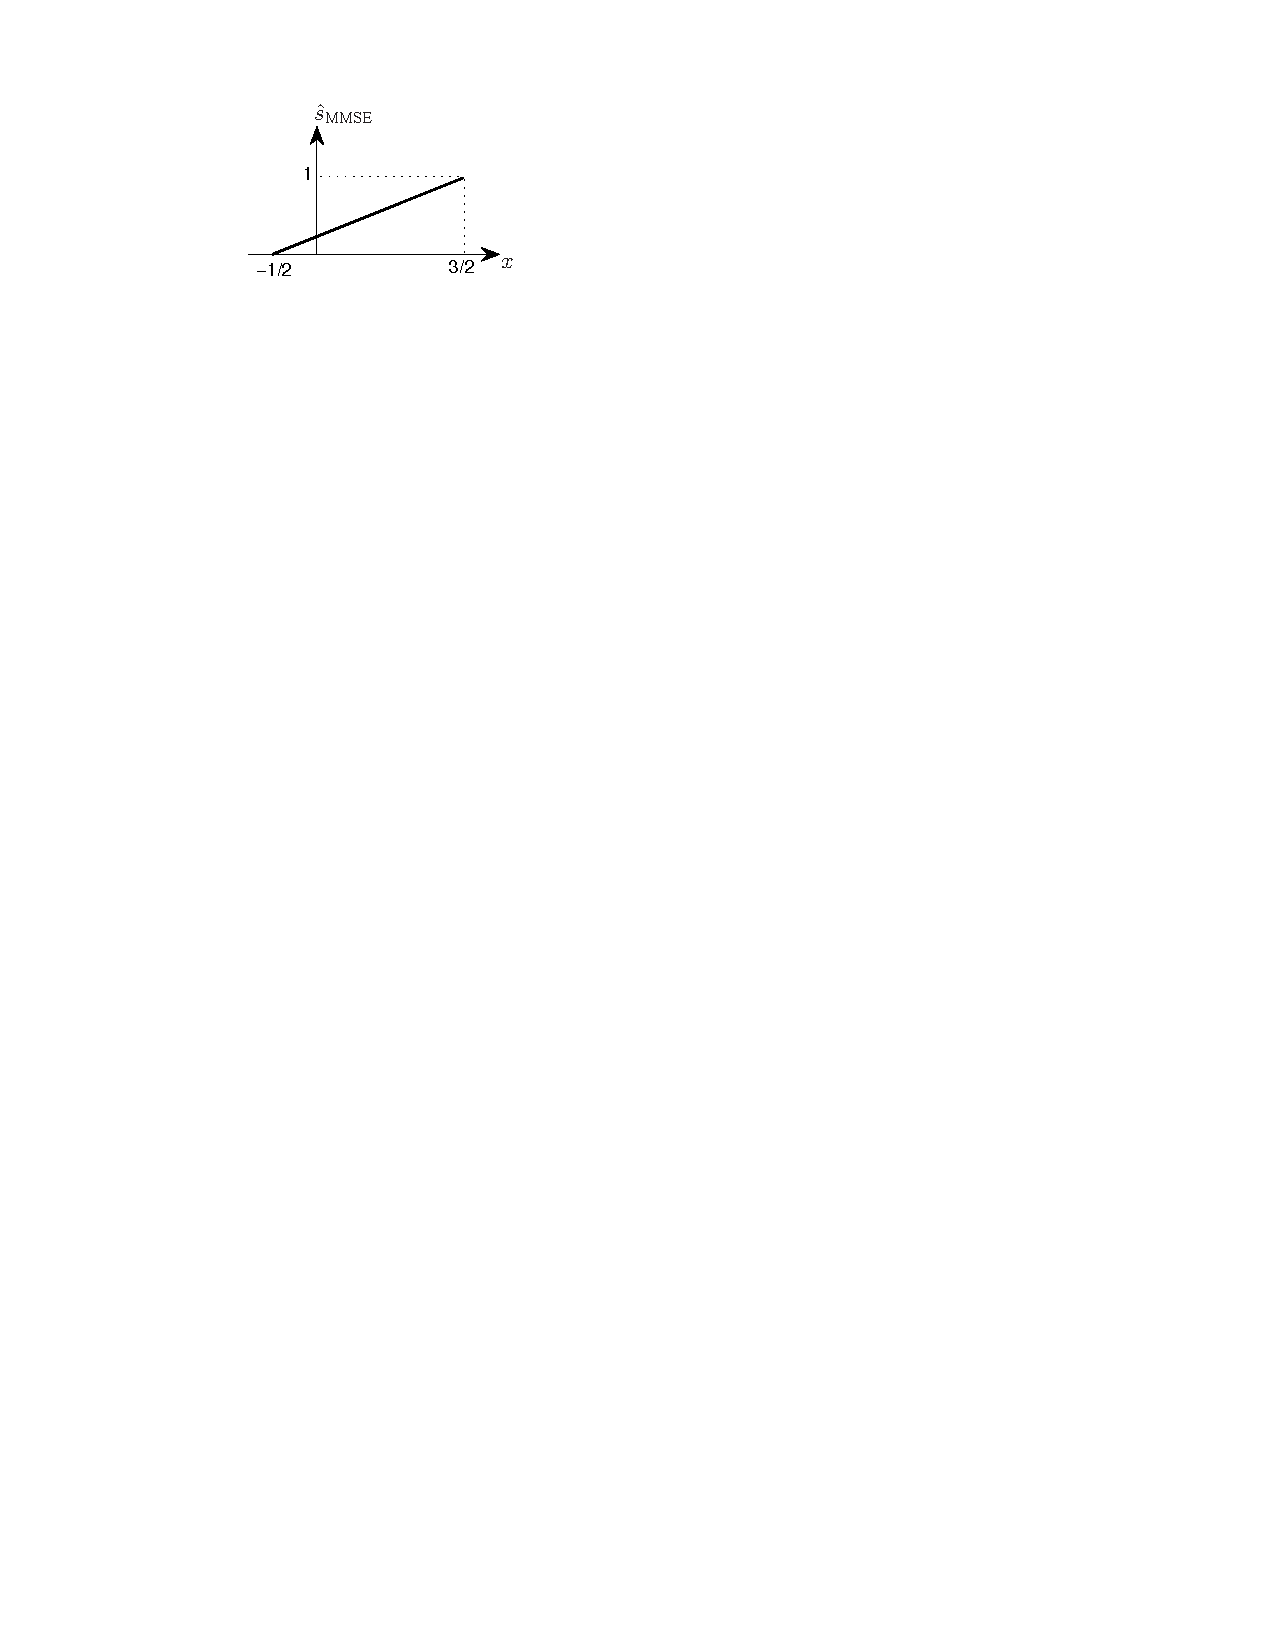
\includegraphics[width=8cm, trim=0 23cm 12cm 2cm]{Figuras/fig3E1}
   
   Las variaciones entre los casos extremos $(\hat{s}_\text{MMSE} (-1/2) = 0, \hat{s}_\text{MMSE} (3/2) = 1)$ se atribuyen linealmente al ruido
\end{solution}

\else

\question Consider an observation
					 $$ X = S + N  $$
					 where $S$ is  a signal contaminated by additive noise $N$, and where $S$ and $N$ are independent of each other, and with probability density functions given by:
				      $$p_S(s) =
					      \left\{\begin{array}{ll}
						  	\displaystyle
								  1, & 0<s<1 \\
	  							  0, & {\mbox{otherwise}} 
	 					 \end{array} 
						  \right. = \Pi (s - 1/2)
				      $$   
				      $$p_N(n) =
					      \left\{\begin{array}{ll}
						  	\displaystyle
								  1, & -1/2<n<1/2 \\
	  							  0, & {\mbox{otherwise}} 
	 					 \end{array} 
						  \right. = \Pi (n)
				      $$   
	 Find the minimum mean square error estimator of $S$, $\hat{S}_\text{MMSE}$. Discuss your result.

\begin{solution}
   $  \hat S_\text{MMSE} = \displaystyle\frac{1}{2} \left(X + \displaystyle\frac{1}{2}\right) \quad  \quad (-1/2 < x <1/2) $    
   
   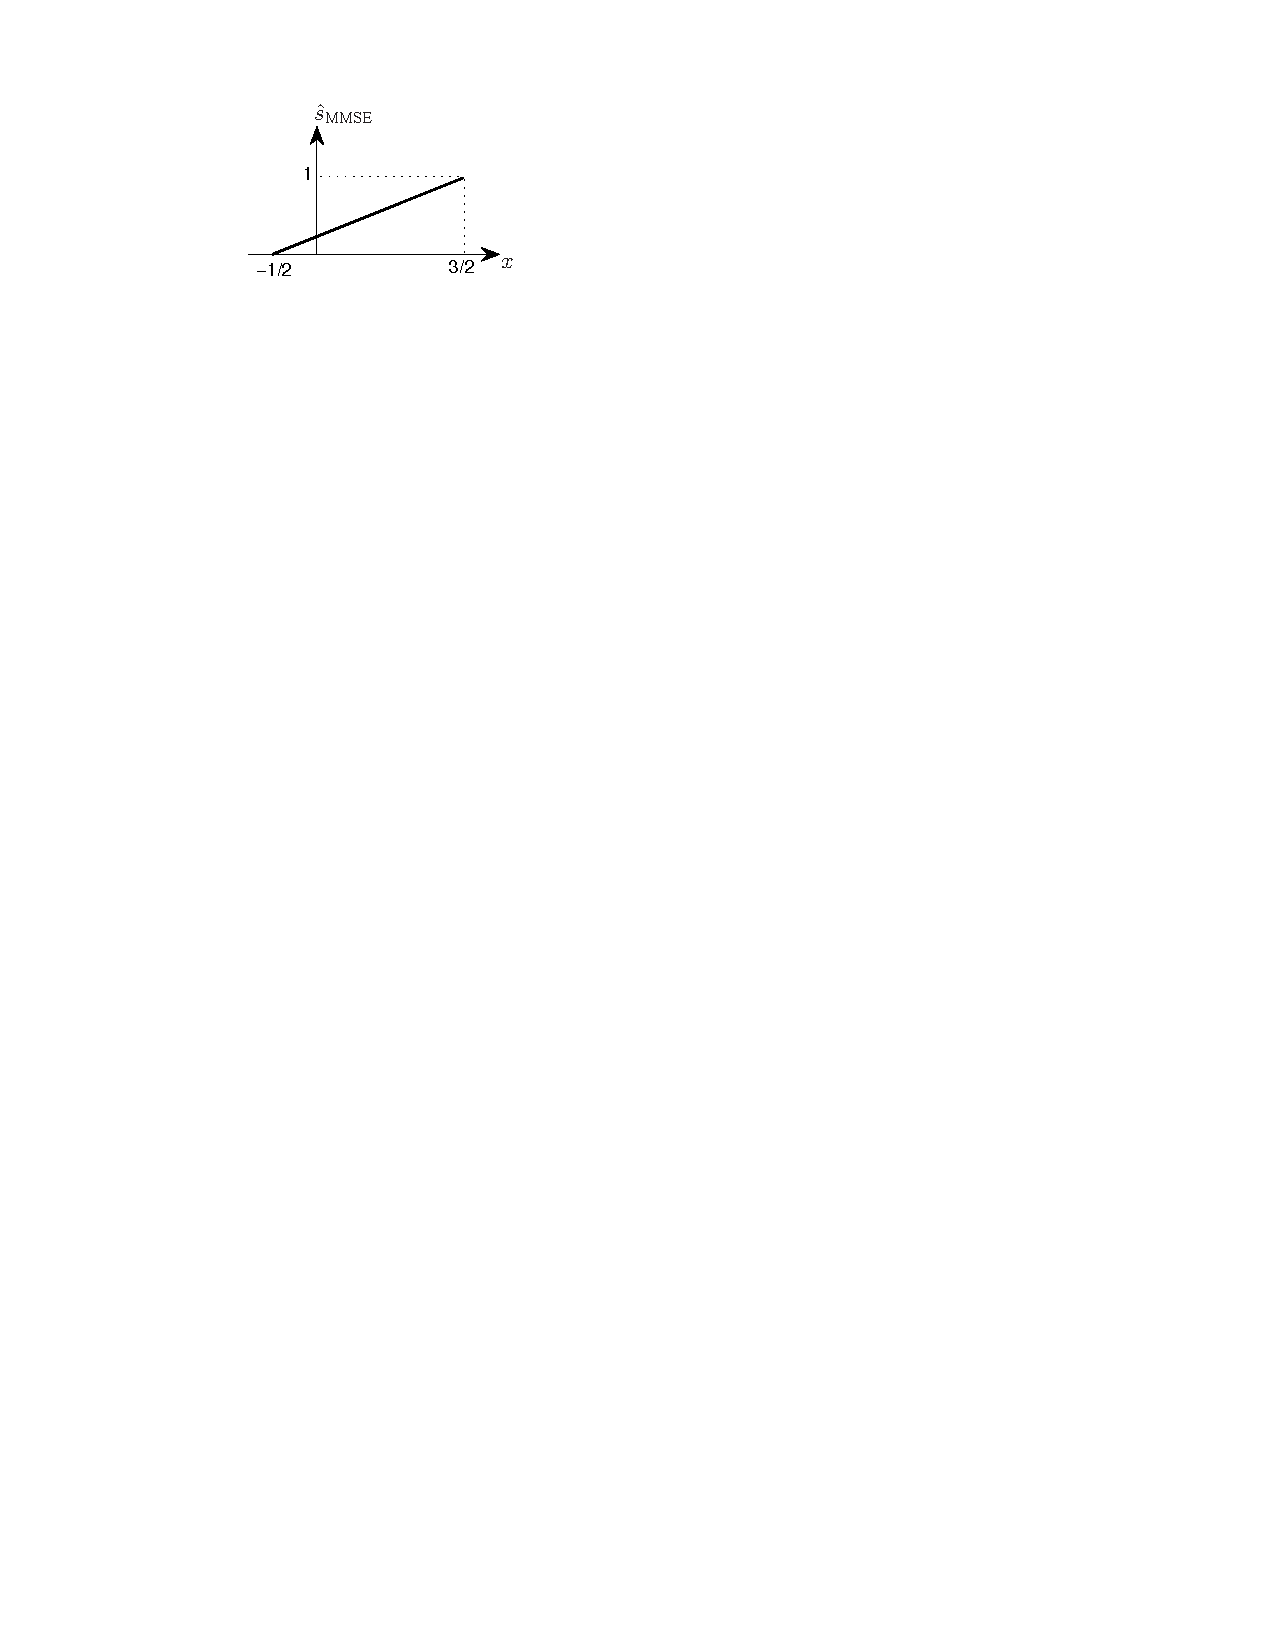
\includegraphics[width=8cm, trim=0 23cm 12cm 2cm]{Figuras/fig3E1}
   
   The linear change of the estimator between its minimum and maximum values $(\hat{s}_\text{MMSE} (-1/2) = 0, \hat{s}_\text{MMSE} (3/2) = 1)$ are due to the addition of uniform noise.
   \end{solution}

\fi

%%%%%%%%%%%%%%%%%%%%%%%%%%%%%%%%%%%%%%%%%%%%%%%%%%%%%%%%%%%%%%%
%  3.E2
\qformat{\textbf{\ej 3.E2 ~~ (1.4)} ~~ \linefill}
\ifspanish

\question Se dispone de $K$ muestras, tomadas independientemente, de una variable $X$ laplaciana $L(m,v)$
\[
  p_X(x) = \frac{1}{\sqrt{2v}} \exp \left( - \sqrt{\frac{2}{v}} |x - m| \right)
\]
Obtener el estimador ML conjunto de $m,v$.

\begin{solution}
  $\begin{array}{lll}\displaystyle
     \hat M_\text{ML} & = &{\mbox{med}}_K \{ X^{(k)}\} \quad {\mbox{(mediana muestral)}} \\
	 & & \\ \displaystyle
     \hat V_\text{ML} & = & \displaystyle\frac{2}{K^2} \left( \sum_k | X^{(k)} - \hat M_\text{ML}| \right)^2
   \end{array}$	 
\end{solution}

\else

\question We have access to $K$ samples independently drawn from a random variable $X$ which follows a Laplace distribution $L(m,v)$
\[
  p_X(x) = \frac{1}{\sqrt{2v}} \exp \left( - \sqrt{\frac{2}{v}} |x - m| \right)
\]
Find the joint ML estimators of $m,v$.

\begin{solution}  $\begin{array}{lll}\displaystyle
     \hat M_\text{ML} & = &{\mbox{med}}_K \{ X^{(k)}\} \quad {\mbox{(sample median)}} \\
	 & & \\ \displaystyle
     \hat V_\text{ML} & = & \displaystyle\frac{2}{K^2} \left( \sum_k | X^{(k)} - \hat M_\text{ML}| \right)^2
   \end{array}$	
   \end{solution}

\fi

%%%%%%%%%%%%%%%%%%%%%%%%%%%%%%%%%%%%%%%%%%%%%%%%%%%%%%%%%%%%%%%
%  4.Q1
\qformat{\textbf{\ej 4.Q1 ~~ (1.5)} ~~ \linefill}
\ifspanish

\question A partir de las variables aleatorias unidimensionales $S$ y $R$, con densidad de probabilidad conjunta
  $$G\left(\textbf{0}, \left[ \begin{array}{cc} 1 & \rho \\ \rho & 1 \end{array} \right]\right),$$
  se forma la observaci\'{o}n  $X = S+ R$

 \begin{parts}
 	\part Determ\'{\i}nese $\hat{S}_\text{MSE}$.
 	\part ¿Era previsible el resultado? (Consid\'{e}rese la relaci\'{o}n que existe entre $ \mathbb E\{ R| x \}$ y $ \mathbb E\{ S | x \}$).
 	\part Calcule el error cuadrático medio.
 \end{parts}

\begin{solution}
  \begin{parts}
  \part $ {\hat S}_\text{MSE} = X/2$
  \part $\mathbb E\{R|x\} =  \mathbb E\{S|x\} \quad {\mbox{(hay total simetr\'{\i}a})}$ \\
  $  \mathbb E\{X|x\} = x = \mathbb E\{S+R|x\} =  \mathbb E\{S|x\} +  \mathbb E\{R|x\}  $
  \part $\mathbb E\left\lbrace \left( S-\hat{S}\right)^2 \right\rbrace =\displaystyle \frac{1}{2} - \displaystyle  \frac{1}{2}  \rho$
\end{parts}
\end{solution}

\else

\question Unidimensional random variables $S$ and $R$ are characterized by the following joint distribution.
  $$
   G\left(\textbf{0}, \left[ \begin{array}{cc} 1 & \rho \\ \rho & 1 \end{array} \right]\right),
  $$
The observable variable is given by $X = S+ R$.

 \begin{parts}
 		\part Obtain the estimator $\hat{S}_\text{MSE}$.
 		\part Was this result to be expected? (Consider the existing relationship between $\mathbb E\{ R| x \}$ and $ \mathbb E\{ S | x \}$).
 		\part Obtain the MSE.
 \end{parts}

\begin{solution}
  \begin{parts}
  \part $ {\hat S}_\text{MSE} = X/2$
  \part $\mathbb E\{R|x\} =  \mathbb E\{S|x\} \quad {\mbox{(since both variables distribute identically given $X$})}$ \\
  $  \mathbb E\{X|x\} = x = \mathbb E\{S+R|x\} =  \mathbb E\{S|x\} +  \mathbb E\{R|x\}  $
  \part $\mathbb E\left\{ \left( S - \hat S\right)^2\right\} = \displaystyle\frac{1}{2} - \displaystyle\frac{1}{2} \rho$
\end{parts}
\end{solution}

\fi

%%%%%%%%%%%%%%%%%%%%%%%%%%%%%%%%%%%%%%%%%%%%%%%%%%%%%%%%%%%%%%%
%  6.E1
\qformat{\textbf{\ej 6.E1 ~~ (1.6)} ~~ \linefill}
\ifspanish

\question Sean  $S$, $X_1$ y $X_2$ tres variables aleatorias de medias nulas tales que:
\begin{itemize}
  \item la matriz de covarianzas de  $X_1$ y $X_2$ es:
  $\textbf{V}_{xx} = \left[ \begin{array}{cc} 1 & \rho \\ \rho & 1 \end{array} \right]$
  \item el vector de covarianzas cruzadas de $S$ con $X$  tiene como expresi\'{o}n:
  $\textbf{v}_{sx} = \left[ \begin{array}{c} 1  \\ 0 \end{array} \right]$
\end{itemize}  
 \begin{parts}
	\part Calc\'{u}lense los coeficientes $w_1$ y $w_2$ del estimador lineal de mínimo error cuadrático medio
	$$\hat{S}_\text{LMSE} = w_0+ w_1 X_1 + w_2 X_2$$
	\part Determ\'{\i}nese el valor cuadr\'{a}tico medio del error de estimaci\'{o}n, $\hat E = S - \hat S_\text{LMSE}$.
 	\item[(c)] Disc\'{u}tase el papel de la variable $X_2$ , que, seg\'{u}n se ve, est\'{a} incorrelacionada con la variable $S$ a estimar.
 \end{parts}  

\begin{solution}
  \begin{parts}
  \part $w_1 = \dfrac{1}{1-\rho^2}    \quad \quad
         w_2 = -\dfrac{\rho}{1-\rho^2}$
  \part $\mathbb E\{ {\hat E}^2\} =  \mathbb E\{S^2\} - \displaystyle\frac{1}{1-\rho^2}$
  \part Interviene combin\'{a}ndose con $X_1$ para conseguir una mayor proyecci\'{o}n de $S$.  
\end{parts}
\end{solution}

\else

\question Let  $S$, $X_1$, and $X_2$ be three zero-mean random variables satisfying:
\begin{itemize}
  \item The covariance matrix of $X_1$ and $X_2$ is:
  $$
   \textbf{V}_{xx} = \left[ \begin{array}{cc} 1 & \rho \\ \rho & 1 \end{array} \right]
  $$

  \item the cross-covariance between $S$ and observation vector $X = [X_1, X_2]^T$ is:
  $$
   \textbf{v}_{sx} = \left[ \begin{array}{c} 1  \\ 0 \end{array} \right]
  $$
\end{itemize}  
 \begin{parts}
 		\part Obtain the coefficients of the linear minimum mean square error estimator
		$$
		   \hat{S}_\text{LMSE} = w_0 + w_1 X_1 + w_2 X_2
		$$
		
 		\part Find the expected quadratic value of the estimation error, $\hat E = S - \hat S_\text{LMSE}$.
 		\part Explain which is the role of variable $X_2$, which, as can be seen, is uncorrelated with the variable to be estimated ($S$).
 \end{parts}  

\begin{solution}
  \begin{parts}
  \part
  $ w_1 = \displaystyle\frac{1}{1-\rho^2};
  \quad \quad
     w_2 = -\displaystyle\frac{\rho}{1-\rho^2};
     \quad \quad
     w_0 = 0$
  \part
  $\mathbb E\{ {\hat E}^2\} =  \mathbb E\{S^2\} - \displaystyle\frac{1}{1-\rho^2}$
  \part $X_2$ is combined with $X_1$ allowing a better approximation of $S$.
\end{parts}
\end{solution}

\fi

%%%%%%%%%%%%%%%%%%%%%%%%%%%%%%%%%%%%%%%%%%%%%%%%%%%%%%%%%%%%%%%
%  6.E3
%\qformat{\textbf{\ej 6.E3 ~~ (1.8)} ~~ \linefill}
%\ifspanish

\question Se presentan en la tabla los valores observados de un \'{\i}ndice $s$ de rendimiento de un proceso 
 qu\'{\i}mico en funci\'{o}n de la medida $x$ de una de las materias primas utilizadas, realiz\'{a}ndose $7$ observaciones 
 por medida.
 \begin{center} 
   \begin{tabular}{|| l |c|c|c|c ||}
     \hline $x$ & 20 & 22 & 24 & 26 \\ \hline \hline
	   $s$ & 120 & 112 & 139 & 140 \\
	       & 106 & 134  & 121  & 152  \\ 
	       & 109 & 120  & 122  & 162  \\
	       & 103 & 119  & 121  & 133  \\
	       & 122 & 120  & 123  & 148  \\
	       & 105 & 112  & 135  & 148  \\
	       & 107 & 121  & 126  & 136  \\ \hline 
   \end{tabular}
 \end{center}
 \begin{parts}
 		\part Determ\'{\i}nese la recta de regresi\'{o}n de $s$ sobre $x$.
 		\part Calc\'{u}lense los residuos.
 \end{parts}  

\begin{solution}
  \begin{parts}
  \part  $
     {\hat s} \simeq 1.2714 + 5.3857 x $
  
 
  \part    \begin{tabular}{|| l |c|c|c|c ||}
     \hline $x$ & 20 & 22 & 24 & 26 \\ \hline \hline
   $\text{residuo}$ & 11.02 & -7.75 & 8.47 & -1.30 \\
	       & -2.98 & 14.25  & -9.53  & 10.70  \\ 
	       & 0.02 & 0.25  & -8.53  & 20.70  \\
	       & -5.98 & -0.75  & -9.53  & -8.30  \\
	       & 13.02 & 0.25  & -7.53  & 6.70  \\
	       & -3.98 & -7.75  & 4.47  & -5.30  \\
	       & -1.98 & 1.25  & -4.53  & -5.30  \\ \hline 
   \end{tabular}
 \end{parts} 
\end{solution}

\else

\question The table below shows the observed values of an index $s$ of efficiency of a chemical process as
a function of the measurement $x$ of one of the raw materials used in the process. 7 observations
are taken for each measurement.
 \begin{center} 
   \begin{tabular}{|| l |c|c|c|c ||}
     \hline $x$ & 20 & 22 & 24 & 26 \\ \hline \hline
	   $s$ & 120 & 112 & 139 & 140 \\
	       & 106 & 134  & 121  & 152  \\ 
	       & 109 & 120  & 122  & 162  \\
	       & 103 & 119  & 121  & 133  \\
	       & 122 & 120  & 123  & 148  \\
	       & 105 & 112  & 135  & 148  \\
	       & 107 & 121  & 126  & 136  \\ \hline 
   \end{tabular}
 \end{center}
 \begin{parts}
 		\part Determine the regression line of $s$ over $x$.
 		\part Calculate the residuals.
 \end{parts}  

\begin{solution}
  \begin{parts}
  \part  $
     {\hat s} \simeq 1.2714 + 5.3857 x $
  
 
  \part    \begin{tabular}{|| l |c|c|c|c ||}
     \hline $x$ & 20 & 22 & 24 & 26 \\ \hline \hline
   $\text{residuals}$ & 11.02 & -7.75 & 8.47 & -1.30 \\
	       & -2.98 & 14.25  & -9.53  & 10.70  \\ 
	       & 0.02 & 0.25  & -8.53  & 20.70  \\
	       & -5.98 & -0.75  & -9.53  & -8.30  \\
	       & 13.02 & 0.25  & -7.53  & 6.70  \\
	       & -3.98 & -7.75  & 4.47  & -5.30  \\
	       & -1.98 & 1.25  & -4.53  & -5.30  \\ \hline 
   \end{tabular}
 
 \end{parts}
 \end{solution}

\fi

%%%%%%%%%%%%%%%%%%%%%%%%%%%%%%%%%%%%%%%%%%%%%%%%%%%%%%%%%%%%%%%
%  6.E5
\qformat{\textbf{\ej 6.E5 ~~ (1.6)} ~~ \linefill}
\ifspanish

\question Se desea estimar la v.a. $S$ a partir de observaciones de las vv.aa. $X_1$ y $X_2$; es decir, obtener
$$
		   \hat{S}_\text{LMSE}(X_1,X_2) = w_0 + w_1 X_1 + w_2 X_2
$$
Las medias de dichas variables son $\mathbb E\{S\}=1$, $\mathbb E\{X_1\}=1$ y $\mathbb E\{X_2\}=0$, y sus correlaciones $ \mathbb E\{S^2\}=4$, $\mathbb E\{X_1^2\}=3$, $\mathbb E\{X_2^2\}=2$, $ \mathbb E\{SX_1\}=2$,
$\mathbb E\{SX_2\}=0$ y $\mathbb E\{X_1 X_2\}=1$.

\begin{parts}
 		\part Calcúlense los coeficientes $\{w_i \},i=0,1,2$, de $\hat{S}_\text{LMSE}(X_1 , X_2)$.
 		\part Como se ha visto en a), $v_{SX_{2}}=0$ ¿Por qué resulta $w_2 \neq 0$?
 		\part Determínese el valor cuadrático medio del error de estimación cometido al usar $\hat{S}_\text{LMSE}(X_1 , X_2)$.
 		\part ¿Cómo y cuánto varía el error cuadrático medio si se utiliza $\hat{S}_\text{LMSE}^{'}(X_1) = w_0^{'} + w_1^{'} X_1 $ en vez de $\hat{S}_\text{LMSE}(X_1 , X_2)$?
\end{parts}

\begin{solution}
  \begin{parts}
 \part  $w_{0}=1/3, \ w_{1}=2/3, \ w_2=-1/3$
 \part  Porque combinar $X_1$ y $X_2$ es mejor que utilizar únicamente $X_1$
 \part $ \mathbb E\{ E^{2}\}=7/3$
 \part ($w^{'}_{0}=1/2; \ w^{'}_{1}=1/2$)\\
  $ \mathbb E\{ E^{'2}\}=3$\\
 Aumenta 2/3 (lo que confirma lo dicho en b))  
 \end{parts}
 \end{solution}

\else

\question We want to design a linear minimum mean square error estimator of a random variable $S$ based on the observation of random variables $X_1$ and $X_2$:
$$
		   \hat{S}_\text{LMSE}(X_1,X_2) = w_0 + w_1 X_1 + w_2 X_2
$$
The means of the random variables are $\mathbb E\{S\}=1$, $\mathbb E\{X_1\}=1$, and $\mathbb E\{X_2\}=0$, whereas the correlations are given by $ \mathbb E\{S^2\}=4$, $\mathbb E\{X_1^2\}=3$, $\mathbb E\{X_2^2\}=2$, $ \mathbb E\{SX_1\}=2$,
$\mathbb E\{SX_2\}=0$, and $\mathbb E\{X_1 X_2\}=1$.

\begin{parts}
 		\part Obtain the optimal coefficients $\{w_i \},i=0,1,2$ of $\hat{S}_\text{LMSE}(X_1 , X_2)$.
 		\part Check that $v_{SX_{2}}=0$.  Why can still be $w_2 \neq 0$?
 		\part Calculate the mean square error incurred by the application of estimator $\hat{S}_\text{LMSE}(X_1 , X_2)$.
 		\part How does the mean square error changes if the estimator $\hat{S}_\text{LMSE}^{'}(X_1) = w_0^{'} + w_1^{'} X_1 $, based on the sole observation of $X_1$, is used instead of $\hat{S}_\text{LMSE}(X_1 , X_2)$?
\end{parts}

\begin{solution}
  \begin{parts}
 \part  $w_{0}=1/3, \ w_{1}=2/3, \ w_2=-1/3$
 \part  Combining $X_1$ and $X_2$ is better than just using $X_1$ (using the geometric analogy of the Orthogonality Principle, the projection space spanned by $X_1$ and $X_2$ is larger than the one spanned by $X_1$ alone).
 \part $ \mathbb E\{ E^{2}\}=7/3$
 \part ($w^{'}_{0}=1/2; \ w^{'}_{1}=1/2$).  $ \mathbb E\{ E^{'2}\}=3$.  It increases by 2/3 (confirming our answer to the previous subquestion).
 \end{parts}
 \end{solution}

\fi

\end{questions}

\end{document}
